%─────Lecture 2──────────────────────────────────────────────────────────────────────────────────────────────────────────────────────────────────────
\chapter{Bond Price Volatility}
\marginpar{\footnotesize\textsf{\raggedright Lecture 2\\ September 17, 2026}}

\source{Slides pp.~92--93}

\begin{flushright}
	\itshape Well, Beethoven, what is this?\footnote{Mass in C major, Op.~86 (1808).}\\
	\upshape --- Attributed to Prince Anton Esterházy

	\medskip

	\itshape You mean to tell me that\\
	the success of my program and my re-election\\
	hinges on the Federal Reserve\\
	and a bunch of f--king bond traders?\\
	\upshape --- Bill Clinton to Robert Rubin, January 7, 1993
\end{flushright}

\bigskip

\noindent The previous chapter answered the question ``what is a bond worth?''.
Given a yield $y$ we can compute a price $P$, and given a price we can solve back for the yield.
This chapter answers the next question, which is the one a risk manager actually loses sleep over: \emph{if the yield moves, how much does the price move?}

The whole chapter is an exercise in Taylor expansion.
Write the price as a function $P(y)$ of the yield; then
\[
	\Delta P \;=\; \frac{\partial P}{\partial y}\,\Delta y
	\;+\; \frac{1}{2}\frac{\partial^{2}P}{\partial y^{2}}\,(\Delta y)^{2}
	\;+\; \cdots
\]
The first-order term, suitably normalised, is called \vocab{duration}; the second-order term, suitably normalised, is called \vocab{convexity}.
Everything else --- Macaulay duration, modified duration, effective duration, dollar duration, $D_{\%}$, effective convexity --- is one of these two numbers in a different set of units, or computed by a different method.
Keeping that map in mind is the best defence against the terminology.

\begin{moral}
	Duration is the first derivative of price with respect to yield; convexity is the second.
	Everything in this chapter is bookkeeping around those two facts.

	\vocab{存續期間}（duration）就是價格對殖利率的一階導數，\vocab{凸性}（convexity）就是二階導數；本章其餘的一切，都只是圍繞這兩件事的記帳工作。
\end{moral}

%─────§ Price volatility───────────────────────────────────────────────────────────────────────────────────────────────────────────────────────────
\section{Price Volatility}

\source{Slides pp.~94--95}

\vocab{Volatility} here measures how bond prices respond to interest rate changes.
It is the key input to the risk management of interest rate-sensitive securities: a desk that holds \$1 billion of bonds needs to know, in dollars, what a one-basis-point move costs it.

The question to make precise is this: \emph{what is the sensitivity of the percentage price change to changes in interest rates?}
Note the two deliberate choices hidden in that sentence.
We measure the response in \emph{percentage} terms, so that bonds of different sizes can be compared, and we measure it against a change in the \emph{yield}, which is the single number we have agreed to summarise the whole discount curve by.

\begin{definition}[Price volatility]
	The \vocab{price volatility} of a security with price $P$ and yield $y$ is
	\begin{equation}
		-\,\frac{\dfrac{\partial P}{\partial y}}{P}. \label{eq:price-vol}
	\end{equation}
\end{definition}

Intuitively, for a small yield move $\Delta y$,
\begin{equation}
	\frac{\Delta P}{P} \;\approx\; -\,\text{price volatility} \times \Delta y. \label{eq:price-vol-approx}
\end{equation}

\begin{remark}
	\eqref{eq:price-vol} 的兩個設計都有理由。

	\textbf{為何要除以 $P$？}
	$\partial P/\partial y$ 的單位是「元 per 單位殖利率」，面額 100 的債券和面額 1{,}000 的同一檔債券會得到差十倍的數字。
	除以 $P$ 之後得到的是\emph{百分比}變化對殖利率變化的敏感度，與部位大小無關，才能拿不同債券互相比較。

	\textbf{為何要加負號？}
	價格對殖利率遞減（$\partial P/\partial y < 0$），加上負號後，\vocab{價格波動性}（price volatility）對一般債券是\emph{正數}，講「這檔債券的波動性是 8」比講「是 $-8$」自然。
	代價是 \eqref{eq:price-vol-approx} 裡必須把負號再寫回去。
\end{remark}

\begin{note}
	\eqref{eq:price-vol} is a \emph{local} statement: it is exact only in the limit $\Delta y \to 0$.
	How badly it fails for a finite $\Delta y$ is precisely what convexity, in \autoref{sec:convexity}, will measure.
\end{note}

%─────§ Price volatility of bonds──────────────────────────────────────────────────────────────────────────────────────────────────────────────────
\section{Price Volatility of a Level-Coupon Bond}

\source{Slides p.~96}

For a level-coupon bond the derivative can be computed in closed form.
Recall from the previous chapter that with $n$ periods to maturity, a coupon $C$ per period, par value $F$, and a \emph{periodic} yield $y$,
\begin{equation}
	P \;=\; \frac{C}{y}\Bigl[\,1-(1+y)^{-n}\,\Bigr] \;+\; F(1+y)^{-n}. \label{eq:bond-price-2}
\end{equation}

\begin{proposition}
	The price volatility of a level-coupon bond is
	\begin{equation}
		-\,\frac{(C/y)\,n - \bigl(C/y^{2}\bigr)\bigl[(1+y)^{n+1}-(1+y)\bigr] - nF}
		{(C/y)\bigl[(1+y)^{n+1}-(1+y)\bigr] + F(1+y)}\,. \label{eq:bond-vol}
	\end{equation}
	Here $F$ is the par value and $C$ is the coupon payment per period.
\end{proposition}

\begin{proof}
	Differentiate \eqref{eq:bond-price-2} term by term:
	\[
		\frac{\partial P}{\partial y}
		= -\frac{C}{y^{2}} + \frac{C}{y^{2}}(1+y)^{-n} + \frac{C}{y}\,n(1+y)^{-n-1} - nF(1+y)^{-n-1}.
	\]
	Multiplying through by $(1+y)^{n+1}$ clears every negative power:
	\[
		(1+y)^{n+1}\frac{\partial P}{\partial y}
		= \frac{C}{y}\,n - \frac{C}{y^{2}}\Bigl[(1+y)^{n+1}-(1+y)\Bigr] - nF,
	\]
	which is the numerator of \eqref{eq:bond-vol}.
	Multiplying \eqref{eq:bond-price-2} by the same factor,
	\[
		(1+y)^{n+1}P = \frac{C}{y}\Bigl[(1+y)^{n+1}-(1+y)\Bigr] + F(1+y),
	\]
	which is the denominator.
	The quotient is therefore $\bigl(\partial P/\partial y\bigr)/P$, and \eqref{eq:bond-vol} is its negative, as \eqref{eq:price-vol} requires.
\end{proof}

Two observations about the formula.

\begin{itemize}[itemsep=0.35em]
	\item \textbf{It simplifies with $C = Fc/m$.}
	      If the bond pays an annual coupon rate $c$ with $m$ payments per year, then $C = Fc/m$, and $F$ divides out of numerator and denominator alike.
	      What is left depends only on $c/m$, $y$ and $n$ --- as it must, since price volatility is a percentage quantity and cannot depend on how big the bond is.

	\item \textbf{It is positive.} For the bond above,
	      \[
		      -\,\frac{\partial P/\partial y}{P} \;>\; 0 ,
	      \]
	      because $P$ is a sum of positive cash flows discounted by $(1+y)^{-i}$, every one of which falls as $y$ rises.
	      Higher yield, lower price: the sign is not an accident but a restatement of the discounting formula.
\end{itemize}

%─────§ Macaulay duration─────────────────────────────────────────────────────────────────────────────────────────────────────────────────────────
\section{Macaulay Duration}

\source{Slides p.~97}

\begin{definition}[Macaulay duration]
	The \vocab{Macaulay duration}\footnote{Frederick Macaulay (1882--1970) in 1938.} (MD) is a weighted average of the times to an asset's cash flows.
	The weights are the cash flows' PVs divided by the asset's price.
	Formally, for cash flows $C_{1},\dots,C_{n}$ at times $1,\dots,n$,
	\begin{equation}
		\mathrm{MD} \;\triangleq\; \frac{1}{P}\sum_{i=1}^{n}\frac{C_{i}}{(1+y)^{i}}\;i . \label{eq:md-def}
	\end{equation}
\end{definition}

The definition really is an average.
Put
\[
	w_{i} \;\triangleq\; \frac{1}{P}\,\frac{C_{i}}{(1+y)^{i}} ,
\]
the fraction of today's price that is accounted for by the $i$th cash flow.
Since $P=\sum_{i} C_{i}(1+y)^{-i}$ we have $\sum_{i} w_{i}=1$, and \eqref{eq:md-def} reads $\mathrm{MD}=\sum_{i} w_{i}\,i$.
So MD is the \emph{centre of mass} of the cash flows when each is given the weight of its present value.

\begin{remark}
	\vocab{麥考利存續期間}（Macaulay duration, MD）在問一句話：\emph{這檔債券的錢，平均要等幾期才拿得到？}

	$i$ 是第 $i$ 筆現金流距今幾期（不是到期日，到期日是 $n$）。
	直接把 $1,\dots,n$ 平均，等於不管每期收到的錢多寡，通通當同一回事；但債券到期那期通常連本金帶票息一起付，金額遠大於中途單純的票息，不該跟其他期一樣輕。所以要用每筆現金流的現值佔總價格的比重 $w_{i}$ 來加權——金額愈大、時間愈近，權重愈大，MD 就愈被拉向那一期。
	這就是 \eqref{eq:md-def} 是\vocab{加權平均}（weighted average）、$w_{i}$ 叫\vocab{現值權重}（PV weight）的原因。

	下面例子裡 $w_{5}=0.744$，於是 MD$=4.34$：比單純平均的 $3$ 大得多（因為多數價值壓在最後一期），又比到期日 $5$ 略小（因為中途先收到票息）。
	把每期現值想成掛在時間軸上的砝碼，MD 就是這根槓桿的平衡點，即\vocab{重心}（centre of mass），見 \autoref{fig:md-balance}。

	這個數字有用，是因為錢等得愈久、折現折得愈兇，價格對殖利率也就愈敏感——所以「平均要等幾期」同時也是「殖利率一動，價格會動多少」的度量，這正是下一小節 \eqref{eq:md-vol} 要證明的事。

	單位是「期」，換算成年要除以每年付息次數 $k$（\autoref{sec:conversion-annual}）。
\end{remark}

\begin{figure}[H]
	\centering
	\begin{tikzpicture}[font=\small]
		% axis
		\draw[-{Stealth[length=6pt]}] (-0.4,0) -- (11.4,0) node[right,font=\footnotesize] {$i$};
		\foreach \x/\lbl in {1.8/1, 3.6/2, 5.4/3, 7.2/4, 9.0/5} {
				\draw (\x,-0.09) -- (\x,0.09);
				\node[below=4pt, font=\footnotesize] at (\x,0) {\lbl};
			}
		% bars: heights proportional to PV weights
		\foreach \x/\h/\w in {1.8/0.418/0.0696, 3.6/0.394/0.0657, 5.4/0.372/0.0620,
				7.2/0.350/0.0584, 9.0/4.466/0.7443} {
				\draw[fill=MidnightBlue!22, draw=MidnightBlue!70]
				(\x-0.28,0) rectangle (\x+0.28,\h);
			}
		\node[above, font=\scriptsize, text=MidnightBlue!60!black] at (1.8,0.42) {$0.070$};
		\node[above, font=\scriptsize, text=MidnightBlue!60!black] at (3.6,0.40) {$0.066$};
		\node[above, font=\scriptsize, text=MidnightBlue!60!black] at (5.4,0.38) {$0.062$};
		\node[above, font=\scriptsize, text=MidnightBlue!60!black] at (7.2,0.36) {$0.058$};
		\node[above, font=\scriptsize, text=MidnightBlue!60!black] at (9.0,4.48) {$0.744$};
		% fulcrum at MD = 4.3422  ->  x = 1.8*4.3422 = 7.816
		\draw[WildStrawberry, thick] (7.816,-0.10) -- ++(-0.30,-0.52) -- ++(0.60,0) -- cycle;
		\node[below=0.62cm, font=\footnotesize, text=WildStrawberry!70!black]
		at (7.816,0) {$\mathrm{MD}=4.34$};
		\draw[Gray!55, -{Stealth[length=5pt]}] (0.55,0) -- (0.55,4.95)
		node[above, font=\footnotesize, text=Gray!60!black] {$w_{i}$};
	\end{tikzpicture}
	\caption{Macaulay duration as a centre of mass. The bars are the PV weights
		$w_{i}$ of a five-period bond with $F=100$, period coupon rate $8\%$ and
		yield $y=6\%$; the balance point sits at $\mathrm{MD}=4.34$ periods, short
		of the maturity $n=5$ because the four coupons pull it left.}
	\label{fig:md-balance}
\end{figure}

\begin{eg}[Not on the slides]
	A five-period bond with $F=100$, coupon $C=8$ per period and periodic yield $y=6\%$ has
	\[
		P = \sum_{i=1}^{4}\frac{8}{1.06^{i}} + \frac{108}{1.06^{5}} = 108.4247 ,
	\]
	with PV weights $w_{1},\dots,w_{5} = 0.0696,\,0.0657,\,0.0620,\,0.0584,\,0.7443$.
	Hence
	\[
		\mathrm{MD} = 1(0.0696)+2(0.0657)+3(0.0620)+4(0.0584)+5(0.7443) = 4.3422 \text{ periods} .
	\]
	Almost three quarters of the price is the final principal repayment, which is why MD sits so close to $n=5$.
\end{eg}

\begin{question}
	What if $C_{i}=(1+c)^{i}$ for some constant $c$, letting $n\to\infty$ and assuming $c>y$?\footnote{Contributed by Mr.~Chen, Yu-Hsing (\texttt{B06901048}, \texttt{R11922045}) on March 3, 2023.}
\end{question}

\begin{proof}[Answer]
	Write $q \triangleq (1+c)/(1+y) > 1$, so that $C_{i}(1+y)^{-i} = q^{i}$.
	Then
	\[
		P = \sum_{i=1}^{n} q^{i} = \frac{q(q^{n}-1)}{q-1} \xrightarrow[\;n\to\infty\;]{} \infty ,
	\]
	and the unnormalised numerator $\sum_{i=1}^{n} i\,q^{i}$ diverges faster still.
	Their ratio behaves like $n$ for large $n$, so $\mathrm{MD}\to\infty$ as well.

	The example is not a curiosity but a warning.
	The weighted-average reading of \eqref{eq:md-def} presumes that the weights $w_{i}$ sum to a finite number; when the coupons grow faster than the discount factor shrinks, the price itself is infinite and there is nothing left to average.
	Any security whose cash flows grow at a rate exceeding its own discount rate has no finite price and no finite duration.
\end{proof}

\subsection{MD as a Measure of Price Volatility}
\label{sec:md-volatility}

\source{Slides p.~98}

Here is the fact that makes MD worth defining: it is the bridge between the ``average waiting time'' picture of \eqref{eq:md-def} and the ``price sensitivity'' picture of \eqref{eq:price-vol}.

\begin{theorem}
	The Macaulay duration, in periods, equals
	\begin{equation}
		\mathrm{MD} \;=\; -(1+y)\,\frac{\partial P}{\partial y}\,\frac{1}{P}. \label{eq:md-vol}
	\end{equation}
\end{theorem}

\begin{proof}
	From $P=\sum_{i=1}^{n} C_{i}(1+y)^{-i}$,
	\[
		\frac{\partial P}{\partial y}
		= -\sum_{i=1}^{n} i\,C_{i}(1+y)^{-i-1}
		= -\frac{1}{1+y}\sum_{i=1}^{n} i\,C_{i}(1+y)^{-i} .
	\]
	Multiply both sides by $-(1+y)/P$:
	\[
		-(1+y)\frac{\partial P}{\partial y}\frac{1}{P}
		= \frac{1}{P}\sum_{i=1}^{n}\frac{C_{i}}{(1+y)^{i}}\,i
		= \mathrm{MD}. \qedhere
	\]
\end{proof}

\begin{intuition}
	\eqref{eq:md-vol} says $\mathrm{MD} = (1+y) \times \text{price volatility}$.
	Two quantities defined for entirely different reasons --- one a statement about \emph{time}, the other a statement about \emph{sensitivity} --- turn out to differ only by the factor $1+y$.

	The reason is visible in the proof: differentiating $(1+y)^{-i}$ brings down exactly the factor $i$, which is the time index.
	Long cash flows are discounted more steeply, so a security's sensitivity to $y$ is governed by how far out its money sits.
\end{intuition}

\subsection{MD of a Level-Coupon Bond}

\source{Slides p.~99}

\begin{proposition}
	The MD of a level-coupon bond is
	\begin{equation}
		\mathrm{MD} \;=\; \frac{1}{P}\left[\;\sum_{i=1}^{n}\frac{iC}{(1+y)^{i}} \;+\; \frac{nF}{(1+y)^{n}}\right]. \label{eq:md-bond}
	\end{equation}
	It can be simplified to
	\begin{equation}
		\mathrm{MD} \;=\; \frac{c(1+y)\bigl[\,(1+y)^{n}-1\,\bigr] + ny(y-c)}
		{cy\bigl[\,(1+y)^{n}-1\,\bigr] + y^{2}} , \label{eq:md-bond-closed}
	\end{equation}
	where $c$ is the \emph{period} coupon rate.
\end{proposition}

\eqref{eq:md-bond} is just \eqref{eq:md-def} with the cash flows of a level-coupon bond written out: a coupon $C$ in each of periods $1,\dots,n$, plus the par value $F$ at period $n$.

For \eqref{eq:md-bond-closed}, write $C=Fc$ and let $A(n)\triangleq\sum_{i=1}^{n}(1+y)^{-i}=\bigl[1-(1+y)^{-n}\bigr]/y$ be the ordinary annuity factor, so \eqref{eq:bond-price-2} reads $P=F\bigl[\,c\,A(n)+(1+y)^{-n}\,\bigr]$.
The bracket in \eqref{eq:md-bond} factors the same way:
\[
	\sum_{i=1}^{n}\frac{iC}{(1+y)^{i}} + \frac{nF}{(1+y)^{n}}
	\;=\; F\left[\,c\sum_{i=1}^{n}\frac{i}{(1+y)^{i}} + \frac{n}{(1+y)^{n}}\,\right] .
\]
So the numerator and the denominator $P$ of \eqref{eq:md-bond} carry the \emph{same} factor $F$, and it cancels --- this is why $F$ disappears.
$C$ disappears too, but only because it was never independent: it enters solely through $C=Fc$, and once $F$ is gone all that is left of it is the rate $c$.
Summing the remaining arithmetic--geometric series and simplifying gives \eqref{eq:md-bond-closed}, which --- exactly as with \eqref{eq:bond-vol} --- depends only on $c$, $y$ and $n$, never on the bond's size.

Two consequences are worth stating separately.

\begin{itemize}[itemsep=0.35em]
	\item \textbf{A coupon bond has $\mathrm{MD}<n$.}
	      If $c>0$ then some of the weight $w_{i}$ sits at times $i<n$, so the centre of mass in \autoref{fig:md-balance} is pulled to the left of $n$.
	\item \textbf{A zero-coupon bond has $\mathrm{MD}=n$.}
	      With $c=0$ there is a single cash flow, $w_{n}=1$, and the average of one number is that number.
	      Its duration \emph{is} its term to maturity.
\end{itemize}

%─────§ Remarks on MD─────────────────────────────────────────────────────────────────────────────────────────────────────────────────────────────
\section{What MD Does and Does Not Mean}
\label{sec:md-caveats}

\subsection{When the Formulas Apply}

\source{Slides p.~100}

\begin{note}
	Formulas \eqref{eq:md-vol} and \eqref{eq:md-bond} hold only if the coupon $C$, the par value $F$, and the maturity $n$ are all independent of the yield $y$ --- that is, only if the cash flow is independent of yields.
\end{note}

This is a far stronger assumption than it looks, and the slides' argument for why deserves unpacking.

Suppose the market yield declines.
Mechanically, \eqref{eq:md-bond-closed} then reports a \emph{longer} MD: lower $y$ discounts the distant cash flows less severely, so the weights $w_{i}$ shift towards large $i$ and the centre of mass moves right.
For a plain bond that is the end of the story, and a longer MD does mean greater price volatility.

But now suppose the security's maturity \emph{itself} shortens when yields fall.
Then the actual price volatility, as originally defined in \eqref{eq:price-vol}, may \emph{decrease} at the very moment the formula says the duration lengthened.
Formula and reality point in opposite directions.

\begin{remark}
	白話翻譯一下上面這段在講什麼。

	MD 的公式（\eqref{eq:md-vol}、\eqref{eq:md-bond}）都偷偷假設了一件事：$C$、$F$、$n$ 這些現金流的\emph{內容}不會因為 $y$ 變動而跟著變——也就是「不管殖利率變成怎樣，這張債券該付多少錢、哪一期付，永遠不變」。
	一般公司債、公債確實如此，但\vocab{可贖回債券}（callable bond）跟房貸抵押證券不是：殖利率一降，發行人可能提前贖回、屋主可能\vocab{提前還款}（prepayment）再融資，現金流本身就跟著 $y$ 一起變了。

	現在把「公式算出來的」跟「實際上發生的」分開看：

	\begin{itemize}[nosep]
		\item \textbf{公式算出來的}：套用 \eqref{eq:md-bond-closed}，殖利率 $y$ 下降 $\to$ 折現折得比較輕 $\to$ 較晚那幾期的權重 $w_i$ 變大 $\to$ MD（加權平均的期數）變長。這一步純粹是代公式，跟債券實際上會不會被贖回無關。
		\item \textbf{實際上發生的}：如果這張債券在殖利率下降時被提前贖回或提前還款，它的壽命反而\emph{縮短}了。壽命一短，價格對利率的敏感度（\eqref{eq:price-vol} 那個真正的定義）通常也跟著下降。
	\end{itemize}

	\textbf{為什麼壽命短，敏感度就低？}
	最乾淨的例子是零息債：$P=F(1+y)^{-n}$，算一下 \eqref{eq:price-vol} 就得到價格波動性 $=n/(1+y)$——敏感度就是到期期數 $n$ 除以 $1+y$，$n$ 愈小，敏感度愈低，一目了然。
	直覺上也對：$n$ 愈小，這筆錢愈快回到你手上，$y$ 的變動只需要「折現少數幾期」，累積效果自然小；$n$ 愈大，同一個 $y$ 的變動要連乘（或連加，在指數上）更多次，效果就被放大。
	一般附息債也是同樣道理：\autoref{sec:md-volatility} 已經證明 MD 就是 $(1+y)\times$ 價格波動性，而 MD 本身是現金流到期期數的加權平均，到期日一旦提前，這個加權平均自然跟著縮小，價格波動性也跟著等比例縮小。
\end{remark}

\subsection{How Not To Think about MD}

\source{Slides p.~101}

The MD has its origin in measuring the length of time a bond investment is outstanding, and the name still carries that connotation.
But it should be seen mainly as measuring \emph{price volatility}, for the simple reason that the temporal reading breaks down in cases the volatility reading handles without complaint.

\begin{itemize}[itemsep=0.35em]
	\item \textbf{Duration can be longer than maturity.}
	      A leveraged inverse floater --- a note whose coupon is, say, $20\% - 2\times$ the reference rate --- behaves like a long position in a fixed-rate bond financed by a short position in a floater.
	      Its price sensitivity can exceed that of \emph{any} fixed-rate bond of the same maturity.
	\item \textbf{Duration can be negative.}
	      An interest-only (IO) strip of a mortgage pool loses value when rates fall, because prepayments cut short the very interest payments it owns.
	      Its price \emph{rises} with yields, so $\partial P/\partial y > 0$ and its duration is negative.
	      \autoref{fig:eff-duration} on p.~\pageref{fig:eff-duration} shows exactly such a price curve.
\end{itemize}

Neither of these makes sense under the maturity interpretation: no security is outstanding for longer than its maturity, and none is outstanding for a negative length of time.
Many, if not most, duration-related terms can only be comprehended as measuring volatility.

\begin{remark}
	簡單說：MD 本質上是「利率敏感度」（sensitivity），「加權平均到期時間」只是現金流固定不變時剛好等於敏感度的副產品；現金流一旦隨 $y$ 變化，MD 就可能跑出時間該有的範圍。

	\begin{itemize}[nosep]
		\item \textbf{槓桿反向浮動利率債券（leveraged inverse floater）}：票息 $=20\%-2\times$ 參考利率。等同於「多一張固定利率債（fixed-rate bond）、用借來的錢放空一張浮動利率債（floater）」——浮動債每期重設票息，久期（duration）近乎 $0$，固定債久期則正常。用槓桿多買固定債、空浮動債對沖，等於把固定債的利率敏感度用槓桿倍數放大，MD 自然能超過同期限的一般定息債。
		\item \textbf{IO strip（interest-only strip，純利息證券）}：只分到房貸池的利息，不分本金。$y$（連帶房貸利率）一下降，屋主\vocab{提前還款}（prepayment，也叫 refinance 轉貸）的比例上升；本金一旦提前還完，後面本該收的利息就直接消失，不只是折現折得少。這個「現金流消失」的損失蓋過折現效果，導致價格跟 $y$ 反向變動，$\partial P/\partial y>0$，MD 變負。
	\end{itemize}
\end{remark}

\begin{moral}
	Read ``duration'' as ``price sensitivity measured in units of time'', never as ``time''.

	把 duration 讀成「以時間為單位表示的價格敏感度」，而不是「時間」。
\end{moral}

%─────§ Conversion───────────────────────────────────────────────────────────────────────────────────────────────────────────────────────────────
\section{Conversion to Annual Units}
\label{sec:conversion-annual}

\source{Slides p.~102}

So far everything has been measured in \emph{periods}, with $y$ the periodic yield.
Market conventions quote years and annual yields, so both formulas need converting.
Let $k$ be the compounding frequency per annum and let $y$ now denote the \emph{annual} yield, so that the periodic yield is $y/k$ and cash flow $i$ arrives at time $i/k$ years.

For the MD to be year-based, modify \eqref{eq:md-bond} to
\begin{equation}
	\frac{1}{P}\left[\;\sum_{i=1}^{n}\frac{i}{k}\,\frac{C}{\bigl(1+\frac{y}{k}\bigr)^{i}}
		\;+\; \frac{n}{k}\,\frac{F}{\bigl(1+\frac{y}{k}\bigr)^{n}}\right] . \label{eq:md-years}
\end{equation}
Nothing has changed except that each time index $i$ has been re-expressed as $i/k$ years.
($n$ itself is still a count of \emph{periods}, not years; only the time label in the numerator has been converted to $i/k$ and $n/k$ years, while the discounting exponent stays in periods.)
Formula \eqref{eq:md-vol} likewise becomes
\begin{equation}
	\mathrm{MD} \;=\; -\Bigl(1+\frac{y}{k}\Bigr)\frac{\partial P}{\partial y}\,\frac{1}{P}. \label{eq:md-vol-years}
\end{equation}
By definition, then,
\[
	\mathrm{MD}\ (\text{in years}) \;=\; \frac{\mathrm{MD}\ (\text{in periods})}{k}.
\]

\begin{remark}
    注意 MD(in periods) 是指每期利率 \(\frac{y}{k}\) 算出來的 md，然後 MD(in year)只是把時間的單位從期換到年，利率還是一樣。 
	三個式子講的是同一件事，只是單位不同，但實務上最常出錯的就是單位。

	\eqref{eq:md-years} 這一步很直覺：$i/k$、$n/k$ 只是把「第 $i$ 期」重新標成「第 $i/k$ 年」，$k$ 是常數可以直接從加總裡拿出來，所以整個式子自然就是 $\mathrm{MD}(\text{periods})/k$，沒有懸念。

	\eqref{eq:md-vol-years} 看起來像是另外冒出來的一個公式，但它\emph{不是}重新定義出來湊答案的，而是可以從 \eqref{eq:md-vol} 用連鎖律（chain rule）硬算出來，結果剛好也等於 $\mathrm{MD}(\text{periods})/k$。推導如下。

	把每期的殖利率記成 $y_{p}=y/k$（也就是 \eqref{eq:md-vol} 裡原本那個 $y$，這裡改名是為了不跟年殖利率 $y$ 搞混）。因為 $P$ 其實是 $y_{p}$ 的函數，$y$ 只是透過 $y_{p}=y/k$ 間接影響 $P$，連鎖律給出
	\[
		\frac{\partial P}{\partial y} \;=\; \frac{\partial P}{\partial y_{p}}\cdot\frac{\partial y_{p}}{\partial y} \;=\; \frac{1}{k}\,\frac{\partial P}{\partial y_{p}} .
	\]
	直覺上：$y$ 動 $1$ 個單位，真正拿去折現的 $y_{p}=y/k$ 只被拖著動 $1/k$ 個單位，所以價格對「年殖利率 $y$」的敏感度，天生就比對「期殖利率 $y_p$」的敏感度小了 $k$ 倍——這就是那個 $1/k$ 的來源，跟前面的係數完全無關。

	把這個關係代進 \eqref{eq:md-vol-years}：
	\[
		-\Bigl(1+\frac{y}{k}\Bigr)\frac{\partial P}{\partial y}\frac{1}{P}
		\;=\; -(1+y_{p})\cdot\frac{1}{k}\frac{\partial P}{\partial y_{p}}\cdot\frac{1}{P}
		\;=\; \frac{1}{k}\underbrace{\left[-(1+y_{p})\frac{\partial P}{\partial y_{p}}\frac{1}{P}\right]}_{=\ \mathrm{MD}(\text{periods})\text{，即 \eqref{eq:md-vol}}}
		\;=\; \frac{\mathrm{MD}(\text{periods})}{k} .
	\]
	注意係數 $\bigl(1+y/k\bigr)$ 只是原本的 $(1+y_{p})$ 換了個寫法而已，並沒有跟著 $k$ 做任何調整；真正帶出 $1/k$ 的，是求導變數從 $y_p$ 換成 $y$ 時連鎖律多乘出來的那個因子。兩者是獨立的兩件事，只是恰好都跟 $k$ 有關，才會讓最後結果乾淨地等於 $\mathrm{MD}(\text{periods})/k$——跟直接把加總式除以 $k$（\eqref{eq:md-years} 的做法）殊途同歸，這正是三個式子彼此一致、講的是同一件事的原因。
\end{remark}

%─────§ Modified duration────────────────────────────────────────────────────────────────────────────────────────────────────────────────────────
\section{Modified Duration}

\source{Slides p.~103}

The factor $1+y$ in \eqref{eq:md-vol} is a nuisance if what one actually wants is the sensitivity itself.
Dividing it out gives the quantity traders quote.

\begin{definition}[Modified duration]
	\begin{equation}
		\text{modified duration} \;\triangleq\; -\,\frac{\partial P}{\partial y}\,\frac{1}{P}
		\;=\; \frac{\mathrm{MD}}{1+y}. \label{eq:mod-dur}
	\end{equation}
\end{definition}

So modified duration is exactly the price volatility \eqref{eq:price-vol} of the first section, under a new name.
By the Taylor expansion,
\begin{equation}
	\text{percent price change} \;\approx\; -\,\text{modified duration} \times \text{yield change}. \label{eq:mod-dur-approx}
\end{equation}

\begin{note}
	Taylor-expanding $P$ to first order, $P(y+\Delta y)\approx P(y)+\frac{\partial P}{\partial y}\Delta y$; dividing by $P(y)$ and substituting \eqref{eq:mod-dur} gives exactly \eqref{eq:mod-dur-approx} --- the same computation that produced \eqref{eq:price-vol-approx}.
	 ``price volatility'' and ``modified duration'' are two names for that one term.
\end{note}

\begin{note}
	Modified duration equals MD under continuous compounding.
	With continuous compounding $P=\sum_{i}C_{i}e^{-y t_{i}}$, so $\partial P/\partial y = -\sum_{i} t_{i}C_{i}e^{-yt_{i}}$ and the ratio $-\bigl(\partial P/\partial y\bigr)/P$ is the PV-weighted average of the $t_{i}$ with no correction factor at all.
	The $1+y$ in \eqref{eq:mod-dur} is an artifact of discrete compounding; it is the discrete analogue of the fact that $\frac{d}{dy}e^{-yt}=-t\,e^{-yt}$ exactly, whereas $\frac{d}{dy}(1+y)^{-i}=-i(1+y)^{-i-1}$ picks up one extra factor of $(1+y)^{-1}$.
\end{note}

\subsection{Example}

\source{Slides p.~104}

\begin{eg}
	Consider a bond whose modified duration is $11.54$ with a yield of $10\%$.
	If the yield increases instantaneously from $10\%$ to $10.1\%$, the approximate percentage price change is
	\[
		-11.54 \times 0.001 = -0.01154 = -1.154\% .
	\]
\end{eg}

\begin{remark}
	注意單位：殖利率從 $10\%$ 升到 $10.1\%$，變化量是 $0.1$ 個百分點，也就是 $\Delta y = 0.001$，即十個\vocab{基點}（basis point, bp），不是 $0.1$。
\end{remark}

\subsection{Modified Duration of a Portfolio}
\label{sec:portfolio-duration}

\source{Slides p.~105}

\begin{proposition}
	By calculus, the modified duration of a portfolio equals
	\begin{equation}
		\sum_{i}\omega_{i}D_{i} , \label{eq:portfolio-dur}
	\end{equation}
	where $D_{i}$ is the modified duration of the $i$th asset and $\omega_{i}$ is the market value of that asset expressed as a percentage of the market value of the portfolio.
\end{proposition}

\begin{proof}
	Let the portfolio value be $V=\sum_{i}P_{i}$ and $\omega_{i}=P_{i}/V$. Then
	\[
		-\frac{1}{V}\frac{\partial V}{\partial y}
		= -\frac{1}{V}\sum_{i}\frac{\partial P_{i}}{\partial y}
		= \sum_{i}\frac{P_{i}}{V}\left(-\frac{1}{P_{i}}\frac{\partial P_{i}}{\partial y}\right)
		= \sum_{i}\omega_{i}D_{i} . \qedhere
	\]
\end{proof}

%─────§ Effective duration───────────────────────────────────────────────────────────────────────────────────────────────────────────────────────
\section{Effective Duration}

\source{Slides p.~106}

Yield changes may alter the cash flow, or the cash flow may be too complex for simple formulas --- exactly the callable bonds and mortgage securities that broke \eqref{eq:md-bond} in \autoref{sec:md-caveats}.
We need a general numerical formula for volatility, one that asks the pricing model rather than a closed form.

\begin{definition}[Effective duration]
	\begin{equation}
		\text{effective duration} \;\triangleq\; \frac{P_{-}-P_{+}}{P_{0}\,(y_{+}-y_{-})} , \label{eq:eff-dur}
	\end{equation}
	where $P_{-}$ is the price if the yield is decreased by $\Delta y$, $P_{+}$ is the price if the yield is increased by $\Delta y$, $P_{0}$ is the initial price, $y$ is the initial yield, and $\Delta y$ is small.
\end{definition}

So $y_{\pm}=y\pm\Delta y$ and $y_{+}-y_{-}=2\Delta y$: \eqref{eq:eff-dur} is the \vocab{central difference} approximation to $-\bigl(\partial P/\partial y\bigr)/P$.
The prices $P_{-},P_{0},P_{+}$ are obtained by re-running the pricing model three times --- with the cash flows allowed to change in response to the yield, which is the whole point.

\source{Slides p.~107}

\begin{figure}[H]
	\centering
	\begin{tikzpicture}
		\begin{axis}[
				width=0.88\textwidth, height=6.8cm,
				xmin=-0.35, xmax=10.9, ymin=0, ymax=0.95,
				axis x line=bottom, axis y line=left,
				axis line style={thin, -{Stealth[length=5pt]}},
				xtick={3.070,4.478,5.872}, xticklabels={$y_{-}$, $y$, $y_{+}$},
				ytick={0.3572,0.7101,0.8252}, yticklabels={$P_{-}$, $P_{0}$, $P_{+}$},
				tick style={draw=none},
				tick label style={font=\small},
				xlabel={Yield}, ylabel={Price},
				label style={font=\footnotesize, text=Gray!60!black},
				every axis y label/.style={at={(ticklabel cs:1.0)}, rotate=0, anchor=south},
				every axis x label/.style={at={(ticklabel cs:1.0)}, anchor=west},
				clip=false,
			]
			% Dotted guides.
			\foreach \xx/\yy in {3.070/0.3572, 4.478/0.7101, 5.872/0.8252} {
				\addplot[Gray!65, densely dotted] coordinates {(\xx,0) (\xx,\yy)};
				\addplot[Gray!65, densely dotted] coordinates {(-0.35,\yy) (\xx,\yy)};
			}
			% A tensioned spline smooths the traced samples while retaining their shape.
			\addplot[MidnightBlue!80!black, very thick, smooth, tension=0.42]
			coordinates {
				(0.021,0.1660) (0.199,0.1647) (0.378,0.1675) (0.556,0.1759) (0.735,0.1901) (0.913,0.2104)
				(1.092,0.2367) (1.271,0.2671) (1.449,0.2992) (1.628,0.3290) (1.806,0.3527) (1.985,0.3689)
				(2.163,0.3766) (2.342,0.3782) (2.521,0.3762) (2.699,0.3715) (2.878,0.3650) (3.056,0.3578)
				(3.070,0.3572) (3.235,0.3542) (3.413,0.3542) (3.592,0.3629) (3.771,0.4015) (3.949,0.5133)
				(4.128,0.6176) (4.306,0.6737) (4.478,0.7101) (4.485,0.7115) (4.663,0.7432) (4.842,0.7680)
				(5.021,0.7879) (5.199,0.8035) (5.378,0.8155) (5.556,0.8215) (5.735,0.8237) (5.872,0.8252)
				(5.913,0.8260) (6.092,0.8224) (6.271,0.8130) (6.449,0.7987) (6.628,0.7802) (6.806,0.7581)
				(6.985,0.7334) (7.163,0.7068) (7.342,0.6786) (7.521,0.6512) (7.699,0.6240) (7.878,0.5984)
				(8.056,0.5748) (8.235,0.5537) (8.413,0.5352) (8.592,0.5195) (8.771,0.5070) (8.949,0.4972)
				(9.128,0.4905) (9.306,0.4865) (9.485,0.4853) (9.663,0.4865) (9.842,0.4902) (10.000,0.4946)
			};
			% The chord whose slope the effective duration measures.
			\addplot[RawSienna, thick] coordinates {(3.070,0.3572) (5.872,0.8252)};
			\addplot[only marks, mark=*, mark size=1.5pt, RawSienna]
			coordinates {(3.070,0.3572) (5.872,0.8252)};
			\draw[RawSienna!55, thin]
			(axis cs:4.471,0.5912) -- (axis cs:6.35,0.40);
			\node[RawSienna!80!black, font=\footnotesize, anchor=west]
			at (axis cs:6.40,0.375) {chord slope $=\dfrac{P_{+}-P_{-}}{y_{+}-y_{-}}$};
		\end{axis}
	\end{tikzpicture}
	\caption{Effective duration reads the slope of the chord through
		$(y_{-},P_{-})$ and $(y_{+},P_{+})$, not of the tangent at $y$. The curve is
		traced from the plot shown in class. It is deliberately badly behaved---a
		plateau on the left, a steep rise through the bracket, and a peak just past
		$y_{+}$---and it is \emph{increasing} in the yield over $[y_{-},y_{+}]$, so
		this security's duration there is negative. No closed-form duration formula
		can handle such a price curve.}
	\label{fig:eff-duration}
\end{figure}

\begin{remark}
	\textbf{為什麼要定義 effective duration？} \eqref{eq:md-bond} 的算法是先把價格寫成 $y$ 的封閉公式，再對 $y$ 解析微分。一旦現金流本身會隨 $y$ 改變——可贖回債被贖回、房貸提前還款——這樣的封閉公式根本寫不出來，\eqref{eq:md-bond} 也就沒有意義（正是 \autoref{sec:md-caveats} 點出的情形）。effective duration 的辦法是繞開微分：把定價模型當黑箱，讓 $y$ 分別偏移 $\pm\Delta y$、現金流也跟著一起變動，重新定價三次得到 $P_{-},P_{0},P_{+}$，再用連接 $(y_{-},P_{-})$ 與 $(y_{+},P_{+})$ 的\emph{割線}斜率去近似 $(y,P_{0})$ 處\emph{切線}斜率 $-\partial P/\partial y$。也就是說，\eqref{eq:eff-dur} 不管定價公式長什麼樣、甚至有沒有公式，都能算——這正是「一個泛用的數值公式」的意思。
	（順帶一提：一般中央差分寫成 $(P_{+}-P_{-})/(y_{+}-y_{-})$ 去近似 $\partial P/\partial y$；\eqref{eq:eff-dur} 的分子把順序反過來寫成 $P_{-}-P_{+}$，分母卻維持 $y_{+}-y_{-}$ 不變，這不是筆誤，而是把 duration 定義裡本來就有的那個負號直接吃進分子，等價於在標準中央差分前面乘上 $-1$。）

	\textbf{這張圖在講什麼？} 橫軸是殖利率 $y$、縱軸是價格 $P$；虛線標出 $(y_{-},P_{-})$、$(y,P_{0})$、$(y_{+},P_{+})$ 三個點。曲線刻意畫得不規則——左邊一段平台、中間陡然爬升、過了 $y_{+}$ 後反而往下掉——用來代表 MBS、\vocab{純息分割債券}（interest-only strip, IO）這類現金流會隨 $y$ 改變的證券，這種形狀一般封閉公式完全處理不了。橙色直線是連接 $(y_{-},P_{-})$ 與 $(y_{+},P_{+})$ 的割線，它的斜率（取負號、除以 $P_{0}$）正是 \eqref{eq:eff-dur} 在算的量。
	在圖上區間 $[y_{-},y_{+}]$ 裡曲線是\emph{遞增}的，即 $P_{-}<P_{+}$，於是 $P_{-}-P_{+}<0$，代入 \eqref{eq:eff-dur} 得到 effective duration $<0$——這就是 \autoref{sec:md-caveats}「duration 可以是負的」那個 IO strip 例子的具體樣子。
\end{remark}

\source{Slides p.~108}

One can compute the effective duration of just about any financial instrument: all it takes is a pricing routine that can be called three times.
An alternative is to use the one-sided difference
\begin{equation}
	\frac{P_{0}-P_{+}}{P_{0}\,\Delta y} , \label{eq:eff-dur-onesided}
\end{equation}
which is more economical --- two model runs instead of three, and $P_{0}$ is usually already known --- but theoretically less accurate.

\begin{note}
	The accuracy claim is the standard one from numerical differentiation.
	Expanding $P(y\pm\Delta y)$ about $y$,
	\[
		\frac{P_{-}-P_{+}}{2\Delta y} = -\frac{\partial P}{\partial y} - \frac{1}{6}\frac{\partial^{3}P}{\partial y^{3}}(\Delta y)^{2}+\cdots,
		\qquad
		\frac{P_{0}-P_{+}}{\Delta y} = -\frac{\partial P}{\partial y} - \frac{1}{2}\frac{\partial^{2}P}{\partial y^{2}}\,\Delta y+\cdots .
	\]
	The central difference loses the first-order error term to symmetry: its leading error is $O\bigl((\Delta y)^{2}\bigr)$ against $O(\Delta y)$ for the one-sided version.
	Halving $\Delta y$ buys a factor of four in one case and only a factor of two in the other.
\end{note}

\begin{remark}
	$P_{0}$ 是現在的價格，通常本來就知道；中央差分 \eqref{eq:eff-dur} 分子不含 $P_{0}$，真正要多算的是 $P_{-}$ 與 $P_{+}$ 兩次；單邊差分 \eqref{eq:eff-dur-onesided} 直接拿現成的 $P_{0}$ 當基準，只需多算一次 $P_{+}$，所以少一次定價。

	不準在哪裡：把 $y$ 對稱地往兩邊推，二階（曲率）誤差在 $P_{-}$ 與 $P_{+}$ 裡符號相反、相減即抵消，只剩三階項，誤差 $O((\Delta y)^{2})$；只往一個方向推就沒有這種抵消，誤差停在 $O(\Delta y)$。把 $\Delta y$ 減半，中央差分誤差縮到 $1/4$、單邊只縮到 $1/2$——這正是「省一次定價」換來的代價。
\end{remark}

%─────§ The practices (duration)─────────────────────────────────────────────────────────────────────────────────────────────────────────────────
\section{The Practices: Duration in Percentage Terms}
\label{sec:practices-d}

\source{Slides p.~109}

Duration is usually expressed in percentage terms --- call it $D_{\%}$ --- for quick mental calculation.\footnote{Neftci (2008): ``Market professionals do not like to use decimal points.''}
The percentage price change expressed in percentage terms is then approximated by
\begin{equation}
	-D_{\%}\times\Delta r \label{eq:dpct}
\end{equation}
when the yield increases instantaneously by $\Delta r\%$.

\begin{remark}
	先說清楚一個容易誤會的地方：$D_{\%}$ 不是把 $D$ 換算成百分比形式後得到的另一個數字。它只是 \eqref{eq:dpct} 這條式子裡的\emph{係數}；式子裡真正換了單位的是 $\Delta r$（百分點）跟價格變化（百分比），不是係數本身。下面會證明 $D_{\%}$ 其實跟原來的 duration 數值完全相同——證完之後的說明會解釋為什麼這件事一點都不奇怪。
\end{remark}

\begin{eg}
	Suppose $D_{\%}=10$ and $\Delta r=2$.
	Price will drop by $20\%$, as $10\times 2=20$.
\end{eg}

\begin{exercise}
	$D_{\%}$ in fact equals the original duration. Prove it!
\end{exercise}

\begin{proof}
	Let $D$ be the modified duration, so that $\Delta P/P \approx -D\,\Delta y$ with $\Delta y$ in decimals.
	Writing the yield change in percentage points, $\Delta r = 100\,\Delta y$, and the price change in percent, $100\,\Delta P/P$, gives
	\[
		100\,\frac{\Delta P}{P} \;\approx\; -D\,(100\,\Delta y) \;=\; -D\,\Delta r .
	\]
	Comparing with \eqref{eq:dpct} yields $D_{\%}=D$.
	The two factors of $100$ --- one on each side --- cancel exactly, which is why the convention costs nothing.
\end{proof}

\begin{remark}
	\textbf{$D_{\%}$ 是哪一種 duration？} 不是新的第五種量。前面算出來的那個數字 $D$——這裡是 modified duration \eqref{eq:mod-dur}，若現金流會隨 $y$ 變就是 effective duration \eqref{eq:eff-dur}——$D_{\%}$ 就是同一個 $D$，數值完全不變，只是換一套單位讀它：把 $\Delta y$（小數）換成以\emph{百分點}記的 $\Delta r=100\,\Delta y$，把 $\Delta P/P$（小數）換成以\emph{百分比}記的 $100\,\Delta P/P$。
\end{remark}

%─────§ Hedging─────────────────────────────────────────────────────────────────────────────────────────────────────────────────────────────────
\section{Hedging}

\source{Slides p.~110}

\vocab{Hedging} offsets the price fluctuations of the position to be hedged by the hedging instrument in the opposite direction, leaving the total wealth unchanged.

\begin{remark}
	\vocab{部位}（position）指你手上持有的一筆資產或負債；\emph{要避險的部位}（the position to be hedged）就是你原本就有、想保護價值的那筆持倉，例如一個債券投資組合。\emph{避險工具}（hedging instrument）是額外配上去的另一筆部位，專門用來抵銷前者的風險，通常是另一種對 $y$ 敏感度相反的證券。

	「往相反方向抵銷」的意思是：$y$ 一變動，原部位賺（賠）多少，避險工具那邊就賠（賺）差不多多少；兩筆加在一起，總財富幾乎不受 $y$ 變動影響——這就是 leaving the total wealth unchanged。「差不多多少」要怎麼配、配多少，就是本節接下來要算的東西。
\end{remark}

Percentages are the wrong unit for that job: two positions of different size with equal and opposite \emph{modified} durations do not cancel.
What must cancel is the change in \emph{dollars}.

\begin{definition}[Dollar duration]
	\begin{equation}
		\text{dollar duration} \;\triangleq\; \text{modified duration} \times \text{price} \;=\; -\frac{\partial P}{\partial y}. \label{eq:dollar-dur}
	\end{equation}
\end{definition}

The approximate dollar price change is then
\begin{equation}
	\text{price change} \;\approx\; -\,\text{dollar duration} \times \text{yield change}. \label{eq:dollar-dur-approx}
\end{equation}
One can hedge a bond portfolio with a dollar duration $D$ by bonds with a dollar duration $-D$: the two first-order terms cancel and the combined position is, to first order, insensitive to $y$.

\begin{intuition}
	Modified duration is a \emph{rate}; dollar duration is a \emph{quantity}.
	Hedging is an accounting identity about quantities, so the hedge ratio must be computed in dollar durations.
\end{intuition}

\begin{note}
	The hedge is only first-order and only instantaneous.
	It fails for large moves --- that is the second-order term, i.e.\ convexity --- and it fails when the two legs' yields do not move together, which no single-$y$ framework can express.
\end{note}

\begin{remark}
	「first-order」「second-order」呼應本章最開頭的泰勒展開 $\Delta P=(\partial P/\partial y)\Delta y+\frac12(\partial^{2}P/\partial y^{2})(\Delta y)^{2}+\cdots$：一階項只跟 $\Delta y$ 成正比，也就是 duration 那一項；二階項跟 $(\Delta y)^{2}$ 成正比，也就是 convexity 那一項。

	怎麼看出避險只做到一階：\eqref{eq:dollar-dur-approx} 這條式子本身就只有一階項，完全沒寫 $(\Delta y)^{2}$ 那一塊。配 $D$ 與 $-D$ 兩筆 dollar duration，只保證兩邊代入 \eqref{eq:dollar-dur-approx} 算出來的一階項互相抵銷；至於兩邊真正的二階項（convexity），公式裡從沒要求它們相等，通常也真的不相等，所以加總後還留著一段沒被抵銷的 $(\Delta y)^{2}$ 尾巴。$\Delta y$ 很小時這尾巴可以忽略，避險看起來完美；$\Delta y$ 一大，這段二階尾巴就顯現出來，避險失靈——這就是「fails for large moves」。

	至於「兩腳殖利率沒有一起動」：\vocab{腳}（leg）就是避險這筆交易的其中一邊——被避險的部位是一腳，拿來避險的工具是另一腳，兩腳各自有自己的價格、自己的殖利率。這是另一個完全不同的限制，跟 order 高低無關：整套 $D$、$-D$ 的算法都假設這兩腳共用同一個 $y$（利率平行移動），$y$ 一變兩腳一起變、變一樣多。如果兩腳的殖利率各自變動、不同步（例如一邊是公司債、一邊是公債，信用利差自己在變），就沒有單一個 $y$ 可以同時代入兩腳的一階分析了。
\end{remark}

%─────§ Convexity───────────────────────────────────────────────────────────────────────────────────────────────────────────────────────────────
\section{Convexity}
\label{sec:convexity}

\source{Slides p.~111}

Duration is the first derivative. The second derivative gets its own name.

\begin{definition}[Convexity]
	\begin{equation}
		\text{convexity (in periods)} \;\triangleq\; \frac{\partial^{2}P}{\partial y^{2}}\,\frac{1}{P}. \label{eq:convexity}
	\end{equation}
\end{definition}

\begin{exercise}
	The convexity of a level-coupon bond is positive. Prove it!
\end{exercise}

\begin{proof}
	Write the coupons and the par value as separate terms,
	\[
		P \;=\; \sum_{i=1}^{n}C_{i}(1+y)^{-i} \;+\; F(1+y)^{-n},
	\]
	where $C_{i}=C$ is the coupon paid at period $i$ and $F$ is the par value returned at maturity.
	Differentiating term by term,
	\[
		\frac{\partial P}{\partial y}
		= -\sum_{i=1}^{n} i\,C_{i}\,(1+y)^{-i-1} \;-\; nF(1+y)^{-n-1},
	\]
	and once more,
	\[
		\frac{\partial^{2}P}{\partial y^{2}}
		= \sum_{i=1}^{n} i(i+1)\,C_{i}\,(1+y)^{-i-2} \;+\; n(n+1)\,F(1+y)^{-n-2} \;>\; 0 ,
	\]
	since $C_{i}\ge 0$, $F\ge 0$, not all of them are zero, and $1+y>0$.
	Dividing by $P>0$ leaves the sign unchanged.
	The argument uses nothing about level coupons: \emph{any} security with non-negative, yield-independent cash flows has positive convexity.
\end{proof}

For a bond with positive convexity, the price rises more for a rate decline than it falls for a rate increase of equal magnitude.
（也就是說，凸性為正的債券，殖利率下降時價格漲的幅度，會大於殖利率上升同樣幅度時價格跌的幅度。）
That asymmetry is the content of \autoref{fig:convexity-taylor}: the true price curve bends away from its own tangent, and it bends \emph{upwards}, so the tangent understates the price on both sides.

\source{Slides p.~112}

\begin{figure}[H]
	\centering
	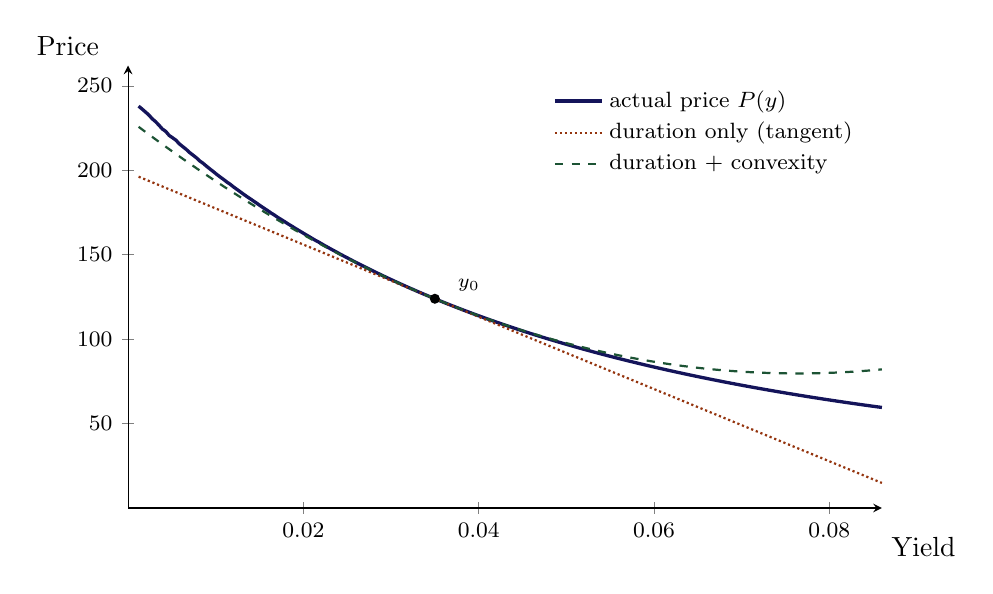
\begin{tikzpicture}
		\begin{axis}[
				width=0.92\textwidth, height=7.2cm,
				xmin=0, xmax=0.086, ymin=0, ymax=262,
				xtick={0.02,0.04,0.06,0.08},
				ytick={50,100,150,200,250},
				xlabel={Yield}, ylabel={Price},
				label style={font=\footnotesize, text=Gray!60!black},
				every axis y label/.style={at={(ticklabel cs:1.0)}, rotate=0, anchor=south},
				every axis x label/.style={at={(ticklabel cs:1.0)}, anchor=west},
				axis x line=bottom, axis y line=left,
				axis line style={thin},
				scaled x ticks=false,
				tick label style={font=\footnotesize,
						/pgf/number format/fixed, /pgf/number format/precision=2},
				yticklabel style={/pgf/number format/precision=0},
				legend style={font=\footnotesize, at={(0.98,0.97)},
						anchor=north east, draw=none, fill=none},
				legend cell align=left,
				clip=false,
			]
			% true price of a 30-period, C = 4.8, F = 100 level-coupon bond
			\addplot[MidnightBlue!80!black, very thick, domain=0.0012:0.086, samples=220]
			{4.8*(1-(1+x)^(-30))/x + 100*(1+x)^(-30)};
			\addlegendentry{actual price $P(y)$}
			% duration-only (tangent at y0 = 0.035)
			\addplot[RawSienna, thick, densely dotted, domain=0.0012:0.086, samples=2]
			{123.9097 - 2138.7667*(x-0.035)};
			\addlegendentry{duration only (tangent)}
			% duration + convexity (quadratic Taylor at y0)
			\addplot[SeaGreen!60!black, thick, dashed, domain=0.0012:0.086, samples=120]
			{123.9097 - 2138.7667*(x-0.035) + 0.5*51715.72*(x-0.035)^2};
			\addlegendentry{duration $+$ convexity}
			\addplot[only marks, mark=*, mark size=1.6pt, black]
			coordinates {(0.035,123.9097)};
			\node[font=\scriptsize, anchor=west] at (axis cs:0.0365,132) {$y_{0}$};
		\end{axis}
	\end{tikzpicture}
	\caption{Price versus yield for a level-coupon bond ($n=30$, $C=4.8$,
		$F=100$), expanded about $y_{0}=3.5\%$. The tangent --- the duration-only
		approximation --- lies below the true curve everywhere, understating the
		gain from a rate fall and overstating the loss from a rate rise. Adding the
		convexity term recovers almost all of the discrepancy over the plotted
		range.}
	\label{fig:convexity-taylor}
\end{figure}

\begin{remark}
	把這張圖讀成三句話：
	\begin{itemize}[nosep]
		\item \textbf{實線}是真正的價格曲線，對殖利率遞減且\emph{向上凸}。
		\item \textbf{點線}是只用 duration 的線性近似，也就是曲線在 $y_{0}$ 的切線。由於曲線是凸的，切線恆在曲線\emph{下方}：殖利率跌時低估漲幅，殖利率漲時高估跌幅——兩邊都對持有人有利，這就是「正凸性是好事」的圖解。
		\item \textbf{虛線}加進了凸性的二次項，在相當寬的範圍內幾乎與實線重合。
	\end{itemize}
	\smallskip
	注意切線與真實曲線的落差隨 $|\Delta y|$ 呈\emph{平方}成長：$\Delta y = 1\%$ 時幾乎看不出來，$\Delta y = 4\%$ 時已經差了幾十塊。這就是為什麼小幅度時可以只用 duration，大幅度時非補上凸性不可。
\end{remark}

\subsection{Consequences and Units}

\source{Slides p.~113}

So between two bonds with the same price and duration, the one with a higher convexity is more valuable.\footnote{Do you spot a problem here (Christensen \& S\o rensen, 1994)?}

Suppose there are $k$ periods per annum.
Convexity measured in periods and convexity measured in years are related by
\begin{equation}
	\text{convexity (in years)} \;=\; \frac{\text{convexity (in periods)}}{k^{2}} . \label{eq:convexity-years}
\end{equation}

\begin{note}
	This is the chain rule, applied twice. Let $u=y/k$ be the periodic yield, so the price is $P(u)$, and let $\widetilde P(y)\triangleq P(y/k)$ be the same price viewed as a function of the annual yield $y$. Since $u=y/k$ is linear in $y$, $du/dy=1/k$ is constant, and
	\[
		\frac{\partial \widetilde P}{\partial y} \;=\; \frac{\partial P}{\partial u}\cdot\frac{du}{dy} \;=\; \frac1k\,\frac{\partial P}{\partial u} ,
	\]
	which is $\mathrm{MD}(\text{years})=\mathrm{MD}(\text{periods})/k$ up to the $(1+u)$-vs.-$1$ normalising factor in \eqref{eq:md-vol}--\eqref{eq:md-vol-years}. Differentiating once more, and noting that $\partial P/\partial u$ is again a function of $u=y/k$, the chain rule applies a \emph{second} time:
	\[
		\frac{\partial^{2}\widetilde P}{\partial y^{2}}
		\;=\; \frac{\partial}{\partial y}\!\left(\frac1k\,\frac{\partial P}{\partial u}\right)
		\;=\; \frac1k\cdot\frac{\partial^{2}P}{\partial u^{2}}\cdot\frac{du}{dy}
		\;=\; \frac{1}{k^{2}}\,\frac{\partial^{2}P}{\partial u^{2}} .
	\]
	Dividing both sides by the same $P$ gives exactly \eqref{eq:convexity-years}: the $k^{2}$ is two factors of $k^{-1}$, one from each application of the chain rule, not an independent convention.

	More generally, this is an induction on the order $r$ of the derivative. The base case $r=1$ is the MD computation above. For the inductive step, suppose $\partial^{r}\widetilde P/\partial y^{r}=k^{-r}\,\partial^{r}P/\partial u^{r}$. The right-hand side is a function of $u=y/k$ composed with $y\mapsto y/k$, so differentiating both sides once more in $y$ picks up one further factor $du/dy=1/k$:
	\[
		\frac{\partial^{r+1}\widetilde P}{\partial y^{r+1}} \;=\; k^{-r}\cdot\frac{\partial^{r+1}P}{\partial u^{r+1}}\cdot\frac{du}{dy} \;=\; k^{-(r+1)}\,\frac{\partial^{r+1}P}{\partial u^{r+1}} .
	\]
	Hence any quantity that is an $r$th derivative with respect to the yield converts between periods and years by a factor of $k^{-r}$: $k^{-1}$ for duration ($r=1$), $k^{-2}$ for convexity ($r=2$).
\end{note}

\begin{remark}
	那個腳註的「問題」在哪裡？

	表面上的推論是：兩檔債券今天價格相同、duration 相同，但一檔凸性較高。
	殖利率不論漲跌，凸性高的那檔表現都不會比較差（漲得多、跌得少）。
	既然如此，它應該比較值錢——但它們今天\emph{價格明明一樣}。這聽起來像是白吃的午餐，也就是\vocab{套利}（arbitrage）機會。

	Christensen 與 S\o rensen（1994）點出的正是這個矛盾：在\vocab{無套利}（no-arbitrage）的\vocab{期限結構}（term structure）模型裡，這種情形不可能持續存在。
	真正的機制是\emph{凸性要付錢買}——市場會把凸性高的債券的殖利率壓低（或說價格推高），高凸性帶來的好處恰好被較低的收益率抵銷。

	更根本的問題出在推論的隱含前提：整條殖利率曲線\emph{平行移動}。
	這個假設本身就與無套利相容不了（若曲線只能平行移動，就能建構出套利部位）。
	一旦改用真正的期限結構模型，「同價同 duration 但凸性較高」的兩檔債券根本不會同時存在於市場上。
\end{remark}

%─────§ Use of convexity─────────────────────────────────────────────────────────────────────────────────────────────────────────────────────────
\section{Use of Convexity}

\source{Slides p.~114}

The approximation $\Delta P/P \approx -\,\text{duration}\times\text{yield change}$ works for small yield changes.
For larger yield changes, keep the next term of the Taylor expansion:
\begin{equation}
	\begin{aligned}
		\frac{\Delta P}{P}
		 & \;\approx\; \frac{\partial P}{\partial y}\,\frac{1}{P}\,\Delta y
		\;+\; \frac{1}{2}\,\frac{\partial^{2}P}{\partial y^{2}}\,\frac{1}{P}\,(\Delta y)^{2} \\[2pt]
		 & \;=\; -\,\text{duration}\times\Delta y
		\;+\; \frac{1}{2}\times\text{convexity}\times(\Delta y)^{2} .
	\end{aligned}\label{eq:taylor2}
\end{equation}
Recall \autoref{fig:convexity-taylor}: the dashed curve \emph{is} \eqref{eq:taylor2}, and the gap between it and the dotted tangent is the convexity term doing its work.

\begin{note}
	Because convexity is positive for an ordinary bond, the second term is positive whichever way $y$ moves.
	The correction always \emph{raises} the predicted price relative to the duration-only estimate --- which is exactly the asymmetry stated on p.~111 of the slides.
\end{note}

%─────§ The practices (convexity)────────────────────────────────────────────────────────────────────────────────────────────────────────────────
\section{The Practices: Convexity in Percentage Terms}

\source{Slides p.~115}

Convexity is likewise usually expressed in percentage terms --- call it $C_{\%}$ --- for quick mental calculation.
The percentage price change expressed in percentage terms is approximated by
\begin{equation}
	-D_{\%}\times\Delta r + C_{\%}\times(\Delta r)^{2}/2 \label{eq:cpct}
\end{equation}
when the yield increases instantaneously by $\Delta r\%$.

\begin{eg}
	Price will drop by $17\%$ if $D_{\%}=10$, $C_{\%}=1.5$ and $\Delta r=2$, because
	\[
		-10\times 2 + \frac{1}{2}\times 1.5\times 2^{2} = -20 + 3 = -17 .
	\]
\end{eg}

\begin{exercise}
	$C_{\%}$ equals convexity divided by $100$. Prove it!
\end{exercise}

\begin{proof}
	Start from \eqref{eq:taylor2} with $\Delta y$ in decimals and substitute $\Delta y = \Delta r/100$:
	\[
		100\,\frac{\Delta P}{P}
		\;\approx\; -D\,(100\,\Delta y) + \frac{1}{2}\,\mathrm{conv}\;\frac{(100\,\Delta y)^{2}}{100}
		\;=\; -D\,\Delta r + \frac{1}{2}\,\frac{\mathrm{conv}}{100}\,(\Delta r)^{2} .
	\]
	Comparing with \eqref{eq:cpct} gives $D_{\%}=D$ as before and $C_{\%}=\mathrm{conv}/100$.
\end{proof}

\begin{remark}
	\textbf{$D_{\%}=D$ 這件事哪裡容易搞錯？} 直覺上很容易以為「掛了 $\%$」代表這個數字本身被換成了百分比形式，所以 $D_\%$ 應該跟 $D$ 長得不一樣（比方乘或除以 $100$）。但 $D_\%$、$C_\%$ 從來不是把 $D$、$\mathrm{conv}$ 本身換算單位，它們只是 \eqref{eq:dpct}、\eqref{eq:cpct} 這兩條式子裡的\emph{係數}；式子裡真正換單位的是變量：輸入端 $\Delta y\to\Delta r=100\Delta y$，輸出端 $\Delta P/P\to 100\,\Delta P/P$。係數本身要變成多少，要看它前面到底黏著幾個 $\Delta y$。
\end{remark}

%─────§ Effective convexity──────────────────────────────────────────────────────────────────────────────────────────────────────────────────────
\section{Effective Convexity}
\label{sec:eff-conv}

\source{Slides p.~116}

Just as effective duration replaced the closed-form first derivative by a difference quotient, effective convexity replaces the second.

\begin{definition}[Effective convexity]
	\begin{equation}
		\text{effective convexity} \;\triangleq\; \frac{P_{+}+P_{-}-2P_{0}}{P_{0}\bigl(0.5\times(y_{+}-y_{-})\bigr)^{2}} , \label{eq:eff-conv}
	\end{equation}
	where $P_{-}$ is the price if the yield is decreased by $\Delta y$, $P_{+}$ the price if it is increased by $\Delta y$, $P_{0}$ the initial price, $y$ the initial yield, and $\Delta y$ small.
\end{definition}

Since $0.5\times(y_{+}-y_{-})=\Delta y$, the denominator is just $P_{0}(\Delta y)^{2}$, and \eqref{eq:eff-conv} is the standard central second difference $\bigl[P_{+}+P_{-}-2P_{0}\bigr]/(\Delta y)^{2}$ normalised by $P_{0}$.
Effective convexity is most relevant when a bond's cash flow is interest rate sensitive --- the callable bonds and mortgage securities for which \eqref{eq:convexity} cannot even be written down, and for which the convexity often turns out \emph{negative}.

\begin{remark}
	\textbf{這條式子在算什麼？} 沿用本章最開頭的泰勒展開 $\Delta P=P'\Delta y+\frac12P''(\Delta y)^{2}+\frac16P'''(\Delta y)^{3}+\cdots$（這裡 $'$ 表示對 $y$ 微分），在 $y$ 兩側各展開一次：
	\[
		P_{+}=P_{0}+P'\Delta y+\tfrac12P''(\Delta y)^{2}+\tfrac16P'''(\Delta y)^{3}+\cdots,
		\qquad
		P_{-}=P_{0}-P'\Delta y+\tfrac12P''(\Delta y)^{2}-\tfrac16P'''(\Delta y)^{3}+\cdots.
	\]
	effective duration 是把這兩式\emph{相減}，讓一階項 $P'\Delta y$ 留下來、其他項互相抵銷或變高階小量。effective convexity 反過來，把兩式\emph{相加}：一階、三階這些奇數階的項符號相反、正好消掉，只留下偶數階：
	\[
		P_{+}+P_{-} = 2P_{0}+P''(\Delta y)^{2}+O\bigl((\Delta y)^{4}\bigr)
		\;\Longrightarrow\;
		\frac{P_{+}+P_{-}-2P_{0}}{(\Delta y)^{2}} = P''+O\bigl((\Delta y)^{2}\bigr).
	\]
	再除以 $P_{0}$，換成跟 \eqref{eq:convexity} 一樣「除以 $P$」的正規化，就得到 \eqref{eq:eff-conv}。所以這條公式跟 effective duration 是同一招的延伸：effective duration 用兩點的\emph{差}逼近一階導數，effective convexity 用三點的\emph{加權和}逼近二階導數。

	\textbf{幾何意義。} $y$ 是 $y_{-}$、$y_{+}$ 的中點，所以連接 $(y_{-},P_{-})$ 與 $(y_{+},P_{+})$ 的割線，在 $y$ 這一點的高度正好是兩端點的平均 $(P_{-}+P_{+})/2$。因此
	\[
		P_{+}+P_{-}-2P_{0} \;=\; 2\left[\frac{P_{-}+P_{+}}{2}-P_{0}\right]
	\]
	就是「割線在 $y$ 處的高度」與「曲線實際在 $y$ 處的高度 $P_{0}$」之間差距的兩倍，見 \autoref{fig:eff-convexity}。曲線向上凸（跟 \autoref{fig:convexity-taylor} 一樣）時，曲線落在割線下方，這個差距是正的，effective convexity 隨之為正；曲線若在這段反而向下凹，差距變負，算出來的 effective convexity 就是負的——這正是 MBS、可贖回債券的凸性常常是負的原因。
\end{remark}

\begin{figure}[H]
	\centering
	\begin{tikzpicture}
		\begin{axis}[
				width=0.65\textwidth, height=6cm,
				xmin=0.3, xmax=3.7, ymin=4.0, ymax=9.0,
				axis x line=bottom, axis y line=left,
				axis line style={thin, -{Stealth[length=5pt]}},
				xtick={1,2,3}, xticklabels={$y_{-}$, $y$, $y_{+}$},
				ytick={4.6,5.6,7.4}, yticklabels={$P_{+}$, $P_{0}$, $P_{-}$},
				tick style={draw=none},
				tick label style={font=\small},
				xlabel={Yield}, ylabel={Price},
				label style={font=\footnotesize, text=Gray!60!black},
				every axis y label/.style={at={(ticklabel cs:1.0)}, rotate=0, anchor=south},
				every axis x label/.style={at={(ticklabel cs:1.0)}, anchor=west},
				clip=false,
			]
			\foreach \xx/\yy in {1/7.4, 2/5.6, 3/4.6} {
					\addplot[Gray!65, densely dotted] coordinates {(\xx,4.0) (\xx,\yy)};
					\addplot[Gray!65, densely dotted] coordinates {(0.3,\yy) (\xx,\yy)};
				}
			\addplot[MidnightBlue!80!black, very thick, domain=0.6:3.4, samples=60] {10-3*x+0.4*x^2};
			\addplot[RawSienna, thick] coordinates {(1,7.4) (3,4.6)};
			\addplot[only marks, mark=*, mark size=1.5pt, black] coordinates {(1,7.4) (2,5.6) (3,4.6)};
			\addplot[only marks, mark=*, mark size=1.3pt, RawSienna] coordinates {(2,6.0)};
			\draw[RawSienna, thick, {Stealth[length=4pt]}-{Stealth[length=4pt]}] (axis cs:2,5.6) -- (axis cs:2,6.0);
			\node[RawSienna!80!black, font=\footnotesize, anchor=west] at (axis cs:2.08,5.8) {$\dfrac{P_{-}+P_{+}}{2}-P_{0}$};
		\end{axis}
	\end{tikzpicture}
	\caption{The chord through $(y_{-},P_{-})$ and $(y_{+},P_{+})$ sits above the curve at the midpoint $y$ whenever the curve is convex there. Effective convexity is, up to the factor $2/\bigl[(\Delta y)^{2}P_{0}\bigr]$, exactly that vertical gap $(P_{-}+P_{+})/2-P_{0}$.}
	\label{fig:eff-convexity}
\end{figure}

How to choose the right $\Delta y$ is a delicate matter.

%─────§ Numerical caveat─────────────────────────────────────────────────────────────────────────────────────────────────────────────────────────
\section{A Numerical Caveat: Second Differences in Floating Point}

\source{Slides p.~117}

The last sentence is not a throwaway remark, and the slides make the point with a deliberately trivial example.
Take $f(x)=x^{2}$, whose second derivative at $x=1$ is exactly $2$, and form the central second difference\footnote{The slide writes the target as $d^{2}f(x)^{2}/dx^{2}$; the quantity actually approximated is $d^{2}f/dx^{2}=2$.}
\[
	\frac{(1+\Delta x)^{2}+(1-\Delta x)^{2}-2}{(\Delta x)^{2}} .
\]
In exact arithmetic the numerator is $2(\Delta x)^{2}$ and the quotient is $2$ for \emph{every} $\Delta x$ --- there is no truncation error at all, since $f$ is a quadratic.
In floating point the answer is a disaster.

\begin{figure}[H]
	\centering
	\begin{tikzpicture}
		\begin{axis}[
				width=0.92\textwidth, height=6.4cm,
				xmin=0, xmax=6.7, ymin=-63, ymax=9,
				xtick={1,2,3,4,5,6},
				xticklabels={$1{\times}10^{-8}$, $2{\times}10^{-8}$, $3{\times}10^{-8}$,
						$4{\times}10^{-8}$, $5{\times}10^{-8}$, $6{\times}10^{-8}$},
				ytick={-60,-50,-40,-30,-20,-10,0},
				xlabel={$\Delta x$}, ylabel={Error},
				label style={font=\footnotesize, text=Gray!60!black},
				every axis y label/.style={at={(ticklabel cs:1.0)}, rotate=0, anchor=south},
				every axis x label/.style={at={(ticklabel cs:1.0)}, anchor=west},
				axis x line=middle, axis y line=left,
				axis line style={thin},
				tick label style={font=\scriptsize},
				clip=false,
			]
			\addplot[MidnightBlue!80!black, thin, mark=none] coordinates {
					(0.2000,-57.511) (0.2252,-45.783) (0.2504,-37.414) (0.2756,-2.000) (0.3008,-2.000) (0.3260,-2.000)
					(0.3512,-2.000) (0.3764,-2.000) (0.4016,-2.000) (0.4268,-2.000) (0.4520,-12.868) (0.4772,-11.751)
					(0.5024,-2.000) (0.5276,-2.000) (0.5528,-2.000) (0.5780,-2.000) (0.6032,-2.000) (0.6284,-2.000)
					(0.6536,-2.000) (0.6788,-6.819) (0.7040,-6.480) (0.7292,-6.176) (0.7544,5.803) (0.7796,5.307)
					(0.8048,-2.000) (0.8300,-2.000) (0.8552,-2.000) (0.8804,-2.000) (0.9056,-2.000) (0.9308,-2.000)
					(0.9560,-2.000) (0.9812,2.613) (1.0064,2.385) (1.0316,-2.000) (1.0568,1.976) (1.0820,1.793)
					(1.1072,1.623) (1.1324,1.463) (1.1576,-2.000) (1.1828,-2.000) (1.2080,-2.000) (1.2332,0.920)
					(1.2584,0.804) (1.2836,0.695) (1.3088,0.593) (1.3340,0.496) (1.3592,0.404) (1.3844,0.317)
					(1.4096,-2.000) (1.4348,-2.000) (1.4600,2.167) (1.4852,2.027) (1.5104,-0.053) (1.5356,-0.117)
					(1.5608,-0.177) (1.5860,-0.235) (1.6112,-0.289) (1.6364,-2.000) (1.6616,-2.000) (1.6868,1.122)
					(1.7120,1.030) (1.7372,0.943) (1.7624,-0.570) (1.7876,-0.610) (1.8128,-0.649) (1.8380,0.629)
					(1.8632,-0.721) (1.8884,-0.755) (1.9136,-0.787) (1.9388,0.363) (1.9640,0.303) (1.9892,0.245)
					(2.0144,0.189) (2.0396,0.135) (2.0648,0.083) (2.0900,0.033) (2.1152,-0.015) (2.1404,-0.061)
					(2.1656,-0.106) (2.1908,-0.149) (2.2160,-0.191) (2.2412,-0.232) (2.2664,-0.271) (2.2916,-0.309)
					(2.3168,-0.345) (2.3420,-0.381) (2.3672,-0.415) (2.3924,-0.448) (2.4176,0.279) (2.4428,0.233)
					(2.4680,0.187) (2.4932,0.143) (2.5184,0.101) (2.5436,0.059) (2.5688,0.019) (2.5940,-0.680)
					(2.6192,-0.705) (2.6444,0.540) (2.6696,0.493) (2.6948,-0.165) (2.7200,-0.199) (2.7452,-0.232)
					(2.7704,-0.264) (2.7956,0.273) (2.8208,-0.326) (2.8460,-0.355) (2.8712,0.155) (2.8964,0.117)
					(2.9216,0.081) (2.9468,0.046) (2.9720,0.011) (2.9972,-0.023) (3.0224,-0.055) (3.0476,-0.087)
					(3.0728,-0.119) (3.0980,-0.149) (3.1232,0.276) (3.1484,0.240) (3.1736,0.205) (3.1988,0.170)
					(3.2240,0.136) (3.2492,0.103) (3.2744,0.071) (3.2996,-0.368) (3.3248,-0.393) (3.3500,0.374)
					(3.3752,0.339) (3.4004,0.304) (3.4256,-0.108) (3.4508,-0.135) (3.4760,-0.162) (3.5012,0.174)
					(3.5264,-0.214) (3.5516,-0.240) (3.5768,0.083) (3.6020,0.054) (3.6272,0.025) (3.6524,-0.003)
					(3.6776,-0.030) (3.7028,-0.057) (3.7280,-0.083) (3.7532,-0.108) (3.7784,-0.134) (3.8036,-0.158)
					(3.8288,0.121) (3.8540,0.093) (3.8792,0.361) (3.9044,0.039) (3.9296,0.013) (3.9548,-0.012)
					(3.9800,-0.038) (4.0052,-0.339) (4.0304,-0.086) (4.0556,-0.110) (4.0808,0.133) (4.1060,0.107)
					(4.1312,0.082) (4.1564,0.056) (4.1816,0.032) (4.2068,0.008) (4.2320,-0.016) (4.2572,-0.040)
					(4.2824,-0.063) (4.3076,0.154) (4.3328,0.129) (4.3580,0.104) (4.3832,0.080) (4.4084,0.057)
					(4.4336,0.033) (4.4588,0.010) (4.4840,-0.233) (4.5092,-0.253) (4.5344,0.160) (4.5596,0.136)
					(4.5848,0.113) (4.6100,0.090) (4.6352,0.067) (4.6604,0.045) (4.6856,0.023) (4.7108,0.001)
					(4.7360,-0.020) (4.7612,-0.041) (4.7864,0.132) (4.8116,0.110) (4.8368,0.088) (4.8620,0.066)
					(4.8872,0.045) (4.9124,0.024) (4.9376,0.004) (4.9628,-0.197) (4.9880,-0.215) (5.0132,0.120)
					(5.0384,0.099) (5.0636,0.078) (5.0888,0.058) (5.1140,0.038) (5.1392,0.018) (5.1644,-0.002)
					(5.1896,-0.021) (5.2148,-0.040) (5.2400,-0.059) (5.2652,0.082) (5.2904,0.063) (5.3156,0.043)
					(5.3408,0.024) (5.3660,0.005) (5.3912,-0.014) (5.4164,-0.032) (5.4416,-0.050) (5.4668,-0.068)
					(5.4920,0.061) (5.5172,0.042) (5.5424,0.024) (5.5676,0.006) (5.5928,-0.012) (5.6180,-0.030)
					(5.6432,-0.048) (5.6684,-0.065) (5.6936,-0.082) (5.7188,-0.099) (5.7440,0.154) (5.7692,0.135)
					(5.7944,-0.016) (5.8196,-0.033) (5.8448,-0.050) (5.8700,0.062) (5.8952,0.045) (5.9204,0.027)
					(5.9456,0.010) (5.9708,-0.007) (5.9960,-0.024) (6.0212,-0.040) (6.0464,-0.056) (6.0716,0.048)
					(6.0968,0.031) (6.1220,0.014) (6.1472,-0.120) (6.1724,-0.135) (6.1976,0.081) (6.2228,0.064)
					(6.2480,0.048) (6.2732,0.031) (6.2984,0.015) (6.3236,-0.001) (6.3488,-0.017) (6.3740,-0.032)
					(6.3992,-0.048) (6.4244,-0.063) (6.4496,0.028) (6.4748,0.119) (6.5000,-0.003)
				};
		\end{axis}
	\end{tikzpicture}
	\caption{The difference between
		$\bigl[(1+\Delta x)^{2}+(1-\Delta x)^{2}-2\bigr]/(\Delta x)^{2}$ and its exact
		value $2$, computed in IEEE double precision. The flat stretches at $-2$ are
		the cases where the numerator underflows to exactly zero; the spikes are the
		cases where it survives as one or two units in the last place.}
	\label{fig:fp-error}
\end{figure}

\begin{remark}
	這個現象叫做\vocab{災難性抵銷}（catastrophic cancellation），值得一步一步看清楚。

	取 $\Delta x \approx 10^{-8}$。在雙精度浮點數中，$1$ 附近的\vocab{機器精度}（machine epsilon）是 $\varepsilon = 2^{-52}\approx 2.22\times 10^{-16}$，也就是說 $1$ 附近能分辨的最小間隔就是這個數量級。

	而 $(1+\Delta x)^{2}+(1-\Delta x)^{2}-2$ 的真值是 $2(\Delta x)^{2}\approx 2\times 10^{-16}$——恰好落在 $\varepsilon$ 的同一個數量級。
	換句話說，我們要算的\emph{整個答案}都藏在最後一個位元裡。
	多數情況下捨入直接把它抹成 $0$，商數變成 $0$，誤差就是 $0-2=-2$（圖中那些平坦段）；偶爾殘留一兩個 ulp，除以 $(\Delta x)^{2}\approx 10^{-16}$ 之後就被放大成 $\pm 10$ 甚至 $-57$ 的巨大誤差（圖中的尖峰）。

	\textbf{推論：$\Delta y$ 不是愈小愈好。}
	把\vocab{截斷誤差}（truncation error）與\vocab{捨入誤差}（round-off error）寫在一起，設 $u$ 為相對捨入誤差的量級：
	\[
		\underbrace{\tfrac{1}{12}\bigl|P^{(4)}\bigr|(\Delta y)^{2}}_{\text{截斷誤差，隨 }\Delta y\text{ 遞減}}
		\;+\;
		\underbrace{\frac{4u\,|P|}{(\Delta y)^{2}}}_{\text{捨入誤差，隨 }\Delta y\text{ 遞增}} .
	\]
	兩者相權，二階差分的最佳步長約為 $\Delta y \sim \varepsilon^{1/4}\approx 1.2\times 10^{-4}$；一階（中央）差分則是 $\Delta y\sim\varepsilon^{1/3}\approx 6\times 10^{-6}$。
	所以 \eqref{eq:eff-conv} 的 $\Delta y$ 取 1 個 basis point（$10^{-4}$）左右通常是合理的，取 $10^{-8}$ 則會得到一堆雜訊。
\end{remark}

This numerical issue is common in financial engineering but does not have general solutions yet.\footnote{See pp.~872ff of the slides.}

%─────§ Rates vs prices─────────────────────────────────────────────────────────────────────────────────────────────────────────────────────────
\section{Interest Rates and Bond Prices: Which Determines Which?}

\source{Slides p.~118}

\begin{question}
	Do interest rates determine bond prices, or do bond prices determine interest rates?\footnote{Contributed by Mr.~Wang, Cheng (\texttt{R01741064}) on March 5, 2014.}
\end{question}

If you have one, you have the other.
Given a price, the yield is the root of \eqref{eq:bond-price-2}; given a yield, the price is its value.
So they are just two names given to the same thing: the \vocab{cost of fund (資金成本)}.

The difference is one of habit rather than of substance:

\begin{itemize}[nosep]
	\item Traders most likely work with prices.
	\item Banks most likely work with interest rates.
\end{itemize}

\begin{moral}
	Price and yield are one quantity in two coordinate systems.
	Duration and convexity are the derivatives that translate between them.

	價格與殖利率是同一個量的兩套座標；duration 與 convexity 就是在兩者之間換算的導數。
\end{moral}

%─────Term Structure of Interest Rates───────────────────────────────────────────────────────────────────────────────────────────────────────────────
\chapter{Term Structure of Interest Rates}

\source{Slides pp.~119--120}

\begin{flushright}
	\itshape Why is it that the interest of money is lower,\\
	when money is plentiful?\\
	\upshape --- Samuel Johnson (1709--1784)

	\medskip

	\itshape If you have money, don't lend it at interest.\\
	Rather, give [it] to someone\\
	from whom you won't get it back.\\
	\upshape --- Thomas Gospel 95
\end{flushright}

\bigskip

\noindent Every formula so far has carried a single interest rate.
One $y$ discounted all of a bond's cash flows in \eqref{eq:pv}; one $y$ was perturbed to get duration and convexity in the last chapter.
That was a convenient fiction, and this chapter retires it.

Money borrowed for three months and money borrowed for thirty years do not cost the same, and the pattern of rates across maturities --- the \vocab{term structure} --- is itself the object to be measured.
The plan is:

\begin{enumerate}[nosep, label=(\arabic*)]
	\item say what the term structure is and what its standard shapes are;
	\item replace the single $y$ by a whole schedule of \vocab{spot rates} $S(1),S(2),\dots$, one per maturity, and show why yield-to-maturity discounting was inconsistent all along;
	\item extract those spot rates from observed bond prices (\vocab{bootstrapping}), and see where that procedure runs into the data;
	\item use the curve to measure credit risk (\vocab{spreads}) and relate it back to the yield curve we started from.
\end{enumerate}

\begin{remark}
	\vocab{信用風險}（credit risk）：發行人到期還不出錢（違約）的風險。公司債可能違約，殖利率因此比公債高，這多出來的部分就是\vocab{利差}（spread），細節見 \autoref{sec:spreads}。
\end{remark}

%─────§ What the term structure is──────────────────────────────────────────────────────────────────────────────────────────────────────────────────
\section{What the Term Structure Is}
\label{sec:what-term-structure}

\source{Slides p.~121}

The term structure is concerned with how interest rates change with maturity.
Concretely, the set of yields to maturity for bonds form the term structure --- subject to two conditions that do all the work:

\begin{itemize}[nosep]
	\item The bonds must be of equal quality.
	\item They differ solely in their terms to maturity.
\end{itemize}

The term structure is fundamental to the valuation of fixed-income securities.

\begin{remark}
	\vocab{期限結構}（term structure）就是「殖利率隨到期日怎麼變化」畫出來的一條曲線——橫軸是到期日，縱軸是殖利率。

	具體做法是拿一群債券各自的到期殖利率當縱軸上的點，但只有兩個條件都成立時，畫出來的才算是期限結構：品質相同、只差到期日。
	這樣才能保證點跟點之間的殖利率差異\emph{純粹來自到期日不同}；若拿信用品質不同的債券比，測到的其實是信用風險（\autoref{sec:spreads}），畫出來的就不是期限結構。

	最後一句「fundamental to valuation」是說：債券價格是把每期現金流分別折現再加總，不同到期日理當用不同的折現率，而期限結構正是提供這些折現率的來源——這也是本章稍後要用一整組 spot rate $S(1),S(2),\dots$ 取代單一 $y$ 的原因。
\end{remark}

\source{Slides p.~122}

Three names get used loosely and are worth separating once and for all:

\begin{itemize}[itemsep=0.35em]
	\item The term ``\vocab{term structure}'' often refers exclusively to the yields of \emph{zero-coupon} bonds.
	      This is the convention adopted here, and the reason will become clear in \autoref{sec:spot-discount}: only a zero has a single, unambiguous date attached to it.
	\item A \vocab{yield curve} plots the yields to maturity of \emph{coupon} bonds against maturity.
	\item A \vocab{par yield curve} is constructed from bonds trading near par.
\end{itemize}

\begin{note}
	這三條曲線是用同一個市場的資料，算出來的三種不同東西。

	一檔 coupon bond 的 yield 為什麼會「混雜」不同到期日的利率：它的 YTM 是用同一個折現率 $y$ 去折現\emph{所有}期數的現金流、再反解出來的單一數字；coupon 越高，越早期的現金流在價格裡佔比越重，YTM 就越偏向那些早期的折現率。換句話說，同樣 $n$ 年到期、但 coupon 不同的兩檔債券，YTM 一般並不相同——同一個到期日底下，YTM 其實不只一個值，會隨挑到哪個 coupon 而變。這就是「yield curve 是 term structure 被混雜後的版本」的意思。

	par yield curve 就是從這些不同的 coupon 裡挑出一個標準答案：要求債券恰好 trade at par，即 $P=F$。由價格公式 \eqref{eq:bond-price-2}，
	\[
		P=\frac{C}{y}\Bigl[1-(1+y)^{-n}\Bigr]+F(1+y)^{-n} ,
	\]
	令 $P=F$，兩邊減去 $F(1+y)^{-n}$、再除以共同的 $\bigl[1-(1+y)^{-n}\bigr]$，直接解出 $F=C/y$，也就是 coupon rate $C/F$ 剛好等於 yield $y$。
	所以「trade at par」不是巧合，而是代數上唯一決定了 coupon 該取多少：對每個到期日，par yield curve 只採用「coupon 恰好等於自己 yield」的那一檔債券，不再讓 coupon 隨便挑——這就是把「混雜」固定下來的意思。實務上很少有債券剛好以 par 交易，所以會取 trading near par 的債券近似，此時 $C/F\approx y$ 只是近似相等，不是恰好相等。

	市面上大多數所謂的「yield curve」，包括 \autoref{fig:ust2015} 裡的美國公債利率曲線，其實都是 par yield curve。
\end{note}

\subsection{The Yield Curve of U.S.\ Treasuries}

\source{Slides p.~123}

\begin{figure}[H]
	\centering
	\begin{tikzpicture}
		\begin{axis}[
				width=0.88\textwidth, height=6.4cm,
				xmin=0, xmax=32, ymin=0, ymax=3.25,
				xtick={5,10,15,20,25,30},
				ytick={0.5,1.0,1.5,2.0,2.5,3.0},
				yticklabel style={/pgf/number format/fixed,
						/pgf/number format/fixed zerofill,
						/pgf/number format/precision=1},
				xlabel={Year}, ylabel={Yield (\%)},
				label style={font=\footnotesize, text=Gray!60!black},
				every axis y label/.style={at={(ticklabel cs:1.0)}, rotate=0, anchor=south},
				every axis x label/.style={at={(ticklabel cs:1.0)}, anchor=west},
				axis x line=bottom, axis y line=left,
				axis line style={thin},
				tick label style={font=\footnotesize},
				clip=false,
			]
			\addplot[MidnightBlue!80!black, thick, smooth] coordinates {
					(0.0833,0.02) (0.25,0.07) (0.5,0.16) (1,0.30) (2,0.68)
					(3,1.03) (5,1.62) (7,2.02) (10,2.27) (20,2.68) (30,2.96)
				};
			\addplot[only marks, mark=o, mark size=2.2pt,
				mark options={draw=Red, line width=0.8pt}] coordinates {
					(0.0833,0.02) (0.25,0.07) (0.5,0.16) (1,0.30) (2,0.68)
					(3,1.03) (5,1.62) (7,2.02) (10,2.27) (20,2.68) (30,2.96)
				};
		\end{axis}
	\end{tikzpicture}
	\caption{Yield curve of U.S.\ Treasuries as of July 24, 2015, as shown in
		class. The circles are the eleven quoted maturities --- 1 and 3 and 6
		months, then 1, 2, 3, 5, 7, 10, 20 and 30 years --- and the line is an
		interpolation through them. Note how unevenly the quotes are spaced: eight
		of the eleven sit inside the first ten years.}
	\label{fig:ust2015}
\end{figure}

\begin{remark}
	這張圖有兩個訊息，一個明顯、一個要留意。

	明顯的是\emph{形狀}：短端幾乎貼地（1 個月只有 $0.02\%$），長端接近 $3\%$，是標準的\vocab{正常}（normal）曲線。
	這是 2015 年的美國——金融海嘯後聯準會把短率壓在零附近已近七年。

	要留意的是\emph{橫軸上的點有多稀疏}。
	市場只在十一個到期日上報價，其中八個擠在前十年；$10$ 年到 $20$ 年之間整整十年沒有任何資料點。
\end{remark}

\subsection{Four Typical Shapes}

\source{Slides p.~124}

\begin{itemize}[nosep]
	\item A \vocab{normal} yield curve is upward sloping.
	\item An \vocab{inverted} yield curve is downward sloping.
	\item A \vocab{flat} yield curve is flat.
	\item A \vocab{humped} yield curve is upward sloping at first but then turns downward sloping.
\end{itemize}

\begin{figure}[H]
	\centering
	\begin{tikzpicture}
		\begin{groupplot}[
				group style={group size=4 by 1, horizontal sep=0.55cm},
				width=0.295\textwidth, height=3.5cm,
				xmin=0, xmax=10.5, ymin=0, ymax=10,
				xtick=\empty, ytick=\empty,
				axis x line=bottom, axis y line=left,
				axis line style={thin, Gray!70},
				title style={font=\footnotesize\sffamily, text=MidnightBlue!70!black,
						yshift=-2pt},
				every axis plot/.append style={MidnightBlue!80!black, very thick},
			]
			\nextgroupplot[title={Normal}]
			\addplot[domain=0.2:10, samples=60] {1.2 + 6.5*(1-exp(-x/3.2))};
			\nextgroupplot[title={Inverted}]
			\addplot[domain=0.2:10, samples=60] {8.2 - 5.8*(1-exp(-x/3.2))};
			\nextgroupplot[title={Flat}]
			\addplot[domain=0.2:10, samples=2] {5};
			\nextgroupplot[title={Humped}]
			\addplot[domain=0.2:10, samples=60] {1.6 + 9.5*(1-exp(-x/1.9)) - 0.62*x};
		\end{groupplot}
	\end{tikzpicture}
	\caption{The four shapes named in class. The horizontal axis is maturity and
		the vertical axis is yield in every panel.}
	\label{fig:four-shapes}
\end{figure}

\begin{remark}
	這四種形狀不只是分類，市場普遍把它們讀成對未來的訊息：
	\begin{itemize}[nosep]
		\item \vocab{正常}（normal）：最常見。長天期資金較貴，通常解讀為經濟擴張、或投資人對長期持有要求額外補償。
		\item \vocab{倒掛}（inverted）：\vocab{短率}（short rate）高於長率。歷史上多次出現在景氣衰退之前，因此被當作預警訊號——市場預期央行日後必須降息。
		\item \vocab{平坦}（flat）：常是正常與倒掛之間的過渡狀態。
		\item \vocab{駝峰}（humped）：中期利率最高，兩端較低。
	\end{itemize}
	倒掛那一條的推理值得補一句。長天期利率大致是「今天的短率」與「市場預期未來各期短率」的平均：把錢鎖十年，跟每期滾動短天期投資十年，預期報酬應該相當，否則資金會往報酬高的那邊跑到兩者拉平為止（這正是之後預期理論的核心）。既然長率是預期短率的平均，長率\emph{低於}今天的短率就只有一種解釋——市場預期未來的短率會比現在低，也就是預期央行日後會降息。而央行通常是在景氣轉弱時才降息，倒掛因此被當成衰退的預警訊號。

	要強調的是：這些都是\emph{經驗上的關聯}，不是本課程要證明的定理。
	曲線形狀為何如此，是 \autoref{sec:ts-problems} 之後幾節（預期理論等）才會處理的問題；此處只需認得這四個名字。
\end{remark}

%─────§ Spot rates─────────────────────────────────────────────────────────────────────────────────────────────────────────────────────────────────
\section{Spot Rates}

\source{Slides p.~125}

\begin{definition}[Spot rate]
	The $i$-period \vocab{spot rate} $S(i)$ is the yield to maturity of an $i$-period zero-coupon bond.
	The PV of one dollar $i$ periods from now is by definition
	\begin{equation}
		\bigl[\,1+S(i)\,\bigr]^{-i}. \label{eq:spot-pv}
	\end{equation}
\end{definition}

Three immediate remarks, all of them from the slides:

\begin{itemize}[itemsep=0.35em]
	\item \eqref{eq:spot-pv} \emph{is} the price of an $i$-period zero-coupon bond, by \eqref{eq:zero-price}.
	      There is nothing to prove: a zero has one cash flow, so its yield and its discount rate are the same number by construction.
	\item The one-period spot rate $S(1)$ is called the \vocab{short rate}.
	\item The \vocab{spot rate curve} --- that is, the term structure, per our convention --- is the plot of spot rates against maturity:
	      \[
		      S(1),\,S(2),\,\ldots,\,S(n).
	      \]
\end{itemize}

\begin{intuition}
	A spot rate is a \emph{price}, not a forecast.
	$S(5)=4\%$ says that one dollar delivered five periods from now trades today at $1.04^{-5}$ dollars; it says nothing about what the short rate will be in five periods' time.

	\vocab{即期利率}（spot rate）是\emph{價格}，不是預測。
	$S(5)=4\%$ 的意思是「五期後的一塊錢今天值 $1.04^{-5}$ 元」，而不是「五期後的短率會是 $4\%$」。
\end{intuition}

%─────§ Problems with the PV formula────────────────────────────────────────────────────────────────────────────────────────────────────────────────
\section{What Is Wrong with Yield-to-Maturity Discounting}
\label{sec:ytm-problem}

\source{Slides p.~126}

In the bond price formula \eqref{eq:pv},
\[
	\sum_{i=1}^{n}\frac{C}{(1+y)^{i}} + \frac{F}{(1+y)^{n}} ,
\]
every cash flow is discounted at the same yield $y$.
Now consider two \vocab{riskless bonds}\footnote{\vocab{Riskless} (or \vocab{default-free}) means the promised cash flows are certain to arrive in full and on time --- the issuer cannot default. Government bonds such as U.S. Treasuries are the standard proxy.} with \emph{different} yields to maturity, the difference arising purely because their cash flows differ:
\begin{align}
	\mathrm{PV}_{1} & = \sum_{i=1}^{n_{1}}\frac{C}{(1+y_{1})^{i}} + \frac{F}{(1+y_{1})^{n_{1}}} , \label{eq:pv1} \\
	\mathrm{PV}_{2} & = \sum_{i=1}^{n_{2}}\frac{C}{(1+y_{2})^{i}} + \frac{F}{(1+y_{2})^{n_{2}}} . \label{eq:pv2}
\end{align}

\begin{note}
	\vocab{無風險債券}（riskless bond，亦稱 default-free bond）指的是\emph{承諾的現金流必定如期足額收到}，發行人不會違約；實務上以公債（如美國國庫券）為代表。

	這個假設在這裡不是裝飾，而是整個論證的關鍵：
	\begin{itemize}[itemsep=0.3em]
		\item 兩檔債券都無風險，才能說它們在第 $i$ 期付的那一塊錢是\emph{同一件商品}——同一天、同樣金額、同樣確定。既然是同一件商品，就不該有兩個價格。
		\item 若兩者信用不同，$y_{1} \neq y_{2}$ 反而理所當然：差額就是\vocab{信用價差}（credit spread），是對違約風險的補償，談不上矛盾。把風險排除後，殖利率的差異就只剩下現金流的時間分佈可以解釋，這正是下一頁要指出的問題所在。
	\end{itemize}

	要注意「無風險」只針對\emph{違約}而言，不表示沒有\vocab{利率風險}：市場利率變動時，債券價格照樣會漲跌（見 \autoref{tab:coupon9}），只是持有到期必定拿得到 $C$ 與 $F$。
\end{note}

\source{Slides p.~127}

The yield-to-maturity methodology discounts their \emph{contemporaneous} cash flows with different rates.
But shouldn't they be discounted at the same rate?

\begin{remark}
	這一頁的投影片只丟出一個問句就結束了，但這是本章的樞紐，值得補完。

	把 \eqref{eq:pv1} 與 \eqref{eq:pv2} 的第 $i$ 期（$i$ 同時小於 $n_1$ 與 $n_2$）拿出來對照：
	兩檔債券都在\emph{同一天}付出\emph{同樣}的 $C$ 元，兩者都\emph{無風險}，可是前者用 $(1+y_1)^{-i}$ 折現、後者用 $(1+y_2)^{-i}$ 折現。
	既然 $y_1 \neq y_2$，同一天、同樣金額、同樣無風險的一塊錢，被賦予了兩個不同的現值。

	這違反\vocab{一價法則}（law of one price）：同一件商品不能有兩個價格。
	而且這不只是美感問題——真有兩個價格就有\vocab{套利}（arbitrage）空間：從便宜的那邊買進未來的一塊錢、往貴的那邊賣出，鎖住無風險利潤。

	\textbf{問題出在哪裡？}
	$y$ 是「把一整串現金流壓成一個數字」的\emph{內部報酬率}，它同時被當成第 1 期到第 $n$ 期的折現率使用。
	但這串現金流的時間分佈（票息高低、到期長短）會影響這個平均值，於是不同的債券得到不同的 $y$。
	換句話說，$y$ 是\emph{債券的}屬性，而折現率應該是\emph{日期的}屬性。

	\textbf{解方}就在下一節：每個日期給它自己的折現率 $S(i)$，與是哪一檔債券付這筆錢無關。
	\vocab{期限結構}（term structure）平坦時（$S(1)=S(2)=\cdots$）兩種作法才會一致；這也解釋了為什麼 $y$ 一直「差不多堪用」——它是對真實折現曲線的一個加權平均近似。
\end{remark}

%─────§ Spot rate discount methodology──────────────────────────────────────────────────────────────────────────────────────────────────────────────
\section{Spot Rate Discount Methodology}
\label{sec:spot-discount}

\source{Slides p.~128}

The repair is to stop thinking of a bond as one instrument with one yield.
A cash flow $C_{1},C_{2},\ldots,C_{n}$ is equivalent to a \emph{package of zero-coupon bonds}, with the $i$th bond paying $C_{i}$ dollars at time $i$.

\begin{figure}[H]
	\centering
	\begin{tikzpicture}[font=\small]
		\draw[-{Stealth[length=6pt]}] (-0.3,0) -- (11.6,0);
		\foreach \x/\lbl/\h in {1.6/1/1.05, 3.6/2/0.85, 5.6/3/0.65, 9.6/n/1.25} {
				\draw[-{Stealth[length=5pt]}, MidnightBlue!80!black, thick]
				(\x,0) -- (\x,\h);
				\node[below=3pt, font=\footnotesize] at (\x,0) {$\lbl$};
			}
		\node[above, font=\footnotesize] at (1.6,1.05) {$C_{1}$};
		\node[above, font=\footnotesize] at (3.6,0.85) {$C_{2}$};
		\node[above, font=\footnotesize] at (5.6,0.65) {$C_{3}$};
		\node[above, font=\footnotesize] at (9.6,1.25) {$C_{n}$};
		\node[font=\footnotesize] at (7.7,0.42) {$\cdots$};
	\end{tikzpicture}
	\caption{A cash flow seen as a package of zero-coupon bonds. Each arrow is a
		separate security, to be priced by its own spot rate.}
	\label{fig:cashflow-package}
\end{figure}

\source{Slides p.~129}

Pricing each arrow at the spot rate matching \emph{its own} date and adding up, a level-coupon bond has the price
\begin{equation}
	P \;=\; \sum_{i=1}^{n}\frac{C}{\bigl[\,1+S(i)\,\bigr]^{i}}
	\;+\; \frac{F}{\bigl[\,1+S(n)\,\bigr]^{n}} . \label{eq:spot-price}
\end{equation}

\begin{itemize}[nosep]
	\item This pricing method incorporates information from the term structure.
	\item It discounts each cash flow at the matching spot rate.
\end{itemize}

\begin{moral}
	The discount rate belongs to the \emph{date}, not to the \emph{bond}.

	折現率屬於\emph{日期}，不屬於\emph{債券}。
\end{moral}

\begin{note}
	Compare \eqref{eq:spot-price} with \eqref{eq:pv}.
	They have the same shape; the only change is that the single $y$ has been replaced by a schedule $S(1),\dots,S(n)$.
	Every complaint of the previous section evaporates: two riskless bonds now discount their common time-$i$ dollar by the same factor, because that factor no longer knows which bond it came from.
\end{note}

%─────§ Discount factors───────────────────────────────────────────────────────────────────────────────────────────────────────────────────────────
\section{Discount Factors}

\source{Slides p.~130}

It is worth giving those common factors a name, because they, rather than the rates, are what the pricing formula actually uses.

\begin{definition}[Discount factors]
	In general, any riskless security having a cash flow $C_{1},C_{2},\ldots,C_{n}$ should have a market price of
	\begin{equation}
		P \;=\; \sum_{i=1}^{n} C_{i}\,d(i) , \label{eq:price-df}
	\end{equation}
	where
	\[
		d(i) \;\triangleq\; \bigl[\,1+S(i)\,\bigr]^{-i} , \qquad i=1,2,\ldots,n ,
	\]
	are called the \vocab{discount factors}.
\end{definition}

\begin{itemize}[nosep]
	\item $d(i)$ is the PV of one dollar $i$ periods from now.
	\item The above formula will be justified later in the course, rather than assumed; the argument is \autoref{thm:pv-justified}.
	\item The discount factors are often interpolated to form a continuous function called the \vocab{discount function}.
\end{itemize}

\begin{note}
	最後一點的意思是：$d(1),d(2),\ldots,d(n)$ 只在\emph{整數期}上有定義，但現實中要折現的日期不見得落在這些格點上（下一期票息可能是 $2.5$ 期後才付）。
	把這串離散的點連成一條曲線 $d(t)$（$t$ 為任意實數），就得到\vocab{折現函數}（discount function）。

	舉個例子。設市場給出
	\[
		S(1)=3\%,\quad S(2)=3.5\%,\quad S(3)=4\% ,
	\]
	亦即
	\[
		d(1)=1.03^{-1}=0.97087,\quad
		d(2)=1.035^{-2}=0.93351,\quad
		d(3)=1.04^{-3}=0.88900 .
	\]
	現在要問：$2.5$ 期後的 $1{,}000$ 元今天值多少？表上沒有 $d(2.5)$，只能內插。最簡單的線性內插是
	\[
		d(2.5) \;\approx\; \frac{d(2)+d(3)}{2} \;=\; 0.91125 ,
	\]
	於是 PV $\approx 1{,}000 \times 0.91125 = 911.25$ 元。

	順帶一提，內插的\emph{對象}會影響答案：若改成先內插利率 $S(2.5) \approx 3.75\%$ 再換算，得
	\[
		d(2.5) = 1.0375^{-2.5} = 0.91207 ,
	\]
	PV 變成 $912.07$ 元，兩者差了約 $0.82$ 元。差距雖小，但在名目金額動輒上億的部位上並非可以忽略；實務上因此不用直線，而是對 $d$（或 $\ln d$）配適三次樣條等較平滑的曲線。
\end{note}

\begin{remark}
	為什麼\vocab{折現因子}（discount factor）要多取一個名字？因為 \eqref{eq:price-df} 對 $d(i)$ 是\emph{線性}的，對 $S(i)$ 卻不是。

	$d(i)$ 是\emph{價格}（今天買一張「$i$ 期後付一元」的憑證要花多少錢），$S(i)$ 只是把同一件事換成年化報酬率的說法。
	凡是關於「一籃子現金流值多少」的敘述，用 $d$ 寫出來都是加權求和，線性代數就能處理；換成 $S$ 就會冒出 $[1+S(i)]^{-i}$ 這種非線性的東西。
	後面的 bootstrapping、避險、以及由債券價格反推曲線的迴歸，全都是在 $d$ 的座標下進行的。

	另外，用 $d$ 寫，\vocab{無套利}（no-arbitrage）的條件也特別乾淨。
	所謂套利，是指一個不必掏錢、卻穩賺不賠的部位（正式定義見 \autoref{sec:arbitrage}）；此處可交易的就是那 $n$ 張零息債券，一組買賣就是一組 $d(i)$ 的加權和。
	於是無套利等價於一句話：$d(i) > 0$——不會有人把未來的一塊錢白送給你。

	至於常見的 $1 > d(1) > d(2) > \cdots$（愈晚的錢愈不值錢），那是\emph{額外}假設「現金可以零成本保存」之後才有的結論，不是無套利本身的內容。
	保管現金其實要成本，這也正是負利率（2015 年起的德國、瑞士公債）能夠存在而不被套利掉的原因。
\end{remark}

%─────§ Bootstrapping──────────────────────────────────────────────────────────────────────────────────────────────────────────────────────────────
\section{Extracting Spot Rates from the Yield Curve}
\label{sec:bootstrap}

\source{Slides p.~131}

The market does not quote $S(1),S(2),\dots$ directly; beyond the very short end it quotes coupon bonds.
Spot rates must therefore be \emph{extracted}, and the extraction is recursive.

\begin{remark}
	「beyond the very short end」指的是殖利率曲線最左端以外的部分。
	最短的那一段（美國約一年以內的 Treasury bills）本身就是零息債券，價格與 $d(1)$ 是同一件事，所以 $S(1)$ 可以直接讀出來；
	但兩年、五年、十年、三十年這些期限，市場上掛牌的都是每期付息的\vocab{附息債券}（coupon bond），沒有純粹「$n$ 期後付一元」的憑證在交易。

	這就是必須\emph{反推}的原因：一張 $n$ 期附息債券的價格是 $d(1),\dots,d(n)$ 的加權和，單一個價格裡混著 $n$ 個未知數。
	但若 $S(1),\dots,S(n-1)$ 已經由更短的債券定出來，那麼這個加權和裡只剩 $d(n)$ 未知，於是一式一未知、可以解出來。
\end{remark}

\begin{itemize}[itemsep=0.35em]
	\item Start with the short rate $S(1)$.
	      Note that short-term Treasuries are zero-coupon bonds, so $S(1)$ can simply be read off.
	\item Compute $S(2)$ from the two-period coupon bond price $P$ by solving
	      \begin{equation}
		      P \;=\; \frac{C}{1+S(1)} \;+\; \frac{C+100}{\bigl[\,1+S(2)\,\bigr]^{2}} . \label{eq:bootstrap-2}
	      \end{equation}
\end{itemize}

The point is that \eqref{eq:bootstrap-2} contains exactly one unknown: $S(1)$ is already known, so the first term is a number, and $S(2)$ can be solved for in closed form.

\source{Slides p.~132}

Inductively, we are given the market price $P$ of the $n$-period coupon bond and
\[
	S(1),\,S(2),\,\ldots,\,S(n-1) .
\]
Then $S(n)$ can be computed from \eqref{eq:spot-price}, repeated here:
\[
	P \;=\; \sum_{i=1}^{n}\frac{C}{\bigl[\,1+S(i)\,\bigr]^{i}}
	\;+\; \frac{F}{\bigl[\,1+S(n)\,\bigr]^{n}} .
\]
The running time can be made to be $O(n)$.
The procedure is called \vocab{bootstrapping}.

\subsection{Why \texorpdfstring{$O(n)$}{O(n)}}

The naive reading of the induction costs $O(n^{2})$: at step $n$ one re-sums $n-1$ discounted coupons.
The saving comes from noticing that the sum only ever grows by one term --- provided we accumulate \emph{discount factors} rather than discounted coupons, since each bond has its own coupon.

Write $A(k) \triangleq \sum_{i=1}^{k} d(i)$ for the running annuity factor.
The $n$-period bond with coupon $C_{n}$ and par $F$ satisfies
\[
	P_{n} \;=\; C_{n}\,A(n-1) \;+\; (C_{n}+F)\,d(n) ,
\]
so that
\begin{equation}
	d(n) \;=\; \frac{P_{n} - C_{n}A(n-1)}{C_{n}+F} ,
	\qquad
	S(n) \;=\; d(n)^{-1/n} - 1 ,
	\qquad
	A(n) \;=\; A(n-1) + d(n) . \label{eq:bootstrap-step}
\end{equation}
Each step is $O(1)$ work, so the whole curve costs $O(n)$.

\begin{algorithm}[H]
	\caption{Bootstrapping the spot rate curve}
	\label{alg:bootstrap}
	\KwIn{prices $P_{1},\ldots,P_{n}$ and coupons $C_{1},\ldots,C_{n}$ of bonds maturing in $1,\ldots,n$ periods; par value $F$}
	\KwOut{spot rates $S(1),\ldots,S(n)$}
	$A := 0$\;
	\For{$k = 1, 2, \ldots, n$}{
		$d := \bigl(P_{k} - C_{k}\,A\bigr)/(C_{k}+F)$\;
		$S(k) := d^{-1/k} - 1$\;
		$A := A + d$\;
	}
	\Return{$S(1),\ldots,S(n)$}\;
\end{algorithm}

\begin{note}
	The $k$th root costs one unit of time under the convention of \autoref{sec:complexity-conv}, where $x^{y}$ was declared a basic operation.
	Without that convention the count would carry an extra factor for the exponentiation --- a good illustration of how much a complexity claim depends on the cost model agreed in advance.
\end{note}

\subsection{A Worked Example}

\begin{eg}[Not on the slides]
	Suppose annual periods, $F=100$, and that the market quotes \emph{par} bonds --- bonds priced at $100$, so that each one's coupon rate equals its own yield --- at
	\[
		y_{1}=3.5\%,\qquad y_{2}=4.0\%,\qquad y_{3}=4.3\%,\qquad y_{4}=4.5\% .
	\]
	For a par bond, $P_{k}=F$ and $C_{k}=F y_{k}$, so \eqref{eq:bootstrap-step} simplifies to
	$d(k) = \bigl[\,1-y_{k}A(k-1)\,\bigr]/(1+y_{k})$.
	Running \autoref{alg:bootstrap}:

	\begin{center}
		\small
		\begin{tabular}{@{}c c c c c@{}}
			\toprule
			$k$ & $y_{k}$ & $A(k-1)$ & $d(k)$   & $S(k)$   \\
			\midrule
			1   & $3.5\%$ & $0$      & $0.966184$ & $3.5000\%$ \\
			2   & $4.0\%$ & $0.966184$ & $0.924378$ & $4.0100\%$ \\
			3   & $4.3\%$ & $1.890561$ & $0.880830$ & $4.3204\%$ \\
			4   & $4.5\%$ & $2.771391$ & $0.837596$ & $4.5301\%$ \\
			\bottomrule
		\end{tabular}
	\end{center}

	Checking the second row against \eqref{eq:bootstrap-2} directly: $100 - 4/1.035 = 96.135266$, and $\bigl(104/96.135266\bigr)^{1/2}-1 = 4.0100\%$ as claimed.
\end{eg}

\begin{remark}
	這張表有兩件事值得盯著看。

	第一，$S(k)$ 一律\emph{高於}同期的 $y_{k}$（$k=1$ 時相等），而且差距隨到期日拉長而擴大：$1$、$10$、$20$、$30$ 個基點。
	這不是巧合，而是 \autoref{sec:spot-vs-yield} 要證明的定理——曲線正常時必然如此。

	第二，$d(k)$ 嚴格遞減（$0.966 > 0.924 > 0.881 > 0.838$），符合前一節說的無套利要求。
	若某組報價算出來的 $d$ 不遞減，那不是曲線奇特，而是資料有問題。
\end{remark}

%─────§ Problems───────────────────────────────────────────────────────────────────────────────────────────────────────────────────────────────────
\section{Some Problems}
\label{sec:ts-problems}

\source{Slides p.~133}

\autoref{alg:bootstrap} is clean; the data are not.

\begin{itemize}[itemsep=0.35em]
	\item Treasuries of the same maturity might be selling at different yields (the \vocab{multiple cash flow problem}).
	\item Some maturities might be missing from the data points (the \vocab{incompleteness problem}).
	\item Treasuries might not be of the same quality.
	\item Interpolation and fitting techniques are needed in practice to create a smooth spot rate curve.\footnote{Often without economic justifications.}
\end{itemize}

\begin{remark}
	逐條說明：

	\textbf{（一）}\vocab{多重現金流問題}（multiple cash flow problem）。
	同一到期日可能有好幾檔公債，票息不同。
	依上一節的分析，票息不同的債券本來就會有不同的 $y$——這正是我們一開始要拋棄 $y$ 的理由。
	麻煩在於它們解出來的 $S(n)$ 也會互相矛盾，於是必須決定採信哪一檔，或做某種平均。

	\textbf{（二）}\vocab{不完整問題}（incompleteness problem）。
	\autoref{alg:bootstrap} 要求每一期 $1,2,\ldots,n$ 都有一檔債券，現實中不可能。
	\autoref{fig:ust2015} 裡 $10$ 年到 $20$ 年之間沒有任何報價，半年期的格點更是大半空著。
	缺的格子只能\emph{猜}。

	\textbf{（三）品質不齊。}
	\vocab{新發行券}（on-the-run）流動性遠優於\vocab{舊券}（off-the-run），殖利率因而偏低；稅負待遇、能否作為附買回擔保品也都造成差異。
	這些價差與期限無關，卻全被算進曲線裡。

	\textbf{（四）}\vocab{插補}（interpolation）。
	前三項的結果是：實務上得到的不是一條曲線，而是一團帶雜訊且有缺口的點。
	要變成可用的 $d(\cdot)$，必須挑一個插補或擬合方法——而那個腳註的力道很重：\emph{通常沒有經濟學上的理由}。
	選哪條曲線，往往只是選哪一種數學上的平滑性。
\end{remark}

\begin{note}
	第（三）條的三種價差各有來歷。

	\textbf{流動性。}價格與殖利率反向，「殖利率低」即「大家願意出更高的價錢」。
	隨時能脫手、買賣價差極窄，本身就是有價值的方便，投資人願意為它多付錢；流動性差的券則必須便宜一點賣，多給的那一截就是\vocab{流動性溢酬}（liquidity premium）。
	交易集中在最新標售的那一檔，它一旦被下一次標售取代就沒人碰了。

	\textbf{稅負。}殖利率是稅前的，投資人在意的是稅後。
	同一到期日、票息不同的兩檔債券，現金流的稅務性質不同——高票息每年課一次利息所得，折價券的報酬大半以到期價差實現、稅率與時點都不一樣——於是稅前價格被推到不同水準。

	\textbf{附買回。}\vocab{附買回}（repo）是「賣出並約定買回」，實質上是拿債券當擔保品借現金，價差即利息。
	若某檔券特別多人想借（例如放空者必須交割它），它的 repo 利率會低於一般擔保品，持有人得以用低於市場的成本取得資金。
	持有它既然多賺這一點，大家就願意接受它債券本身的殖利率低一些；不被接受當擔保品的券則反過來要賣便宜。
\end{note}

\subsection{Which One?}

\source{Slides p.~134}

The incompleteness problem is worth seeing rather than reading about.
Here are the same eleven observations of \autoref{fig:ust2015}, joined three different ways.

\begin{figure}[H]
	\centering
	\begin{tikzpicture}
		\begin{groupplot}[
				group style={group size=3 by 1, horizontal sep=1.05cm},
				width=0.37\textwidth, height=4.1cm,
				xmin=0, xmax=32, ymin=0, ymax=3.25,
				xtick={5,10,15,20,25,30},
				ytick={0.5,1.0,1.5,2.0,2.5,3.0},
				yticklabel style={/pgf/number format/fixed,
						/pgf/number format/fixed zerofill,
						/pgf/number format/precision=1},
				axis x line=bottom, axis y line=left,
				axis line style={thin},
				tick label style={font=\scriptsize},
				title style={font=\footnotesize\sffamily, text=MidnightBlue!70!black},
			]
			\nextgroupplot[title={piecewise constant}]
			\addplot[MidnightBlue!60, very thick, const plot] coordinates {
					(0.0833,0.02) (0.25,0.07) (0.5,0.16) (1,0.30) (2,0.68)
					(3,1.03) (5,1.62) (7,2.02) (10,2.27) (20,2.68) (30,2.96)};
			\addplot[only marks, mark=*, mark size=1.1pt, black] coordinates {
					(0.0833,0.02) (0.25,0.07) (0.5,0.16) (1,0.30) (2,0.68)
					(3,1.03) (5,1.62) (7,2.02) (10,2.27) (20,2.68) (30,2.96)};
			\nextgroupplot[title={piecewise linear}]
			\addplot[MidnightBlue!60, very thick] coordinates {
					(0.0833,0.02) (0.25,0.07) (0.5,0.16) (1,0.30) (2,0.68)
					(3,1.03) (5,1.62) (7,2.02) (10,2.27) (20,2.68) (30,2.96)};
			\addplot[only marks, mark=*, mark size=1.1pt, black] coordinates {
					(0.0833,0.02) (0.25,0.07) (0.5,0.16) (1,0.30) (2,0.68)
					(3,1.03) (5,1.62) (7,2.02) (10,2.27) (20,2.68) (30,2.96)};
			\nextgroupplot[title={smooth spline}]
			\addplot[MidnightBlue!60, very thick, smooth] coordinates {
					(0.0833,0.02) (0.25,0.07) (0.5,0.16) (1,0.30) (2,0.68)
					(3,1.03) (5,1.62) (7,2.02) (10,2.27) (20,2.68) (30,2.96)};
			\addplot[only marks, mark=*, mark size=1.1pt, black] coordinates {
					(0.0833,0.02) (0.25,0.07) (0.5,0.16) (1,0.30) (2,0.68)
					(3,1.03) (5,1.62) (7,2.02) (10,2.27) (20,2.68) (30,2.96)};
		\end{groupplot}
	\end{tikzpicture}
	\caption{Which one? Three curves through the identical eleven quotes of
		\autoref{fig:ust2015}; the horizontal axis is the maturity in years and
		the vertical axis the yield in percent, as before. Every one of them
		reprices all observed bonds exactly; they disagree about everything in
		between.}
	\label{fig:which-one}
\end{figure}

\begin{moral}
	The data fix the curve only where the data are.
	Everywhere else the curve is an assumption --- and any security priced off that stretch inherits it.

	資料只能決定有資料的地方；其餘部分是假設。凡是用那段曲線定價的商品，都繼承了這個假設。
\end{moral}

%─────§ Spreads───────────────────────────────────────────────────────────────────────────────────────────────────────────────────────────────────
\section{Yield Spread and Static Spread}
\label{sec:spreads}

Everything so far assumed riskless cash flows.
A corporate bond promises the same shape of cash flow but may not deliver, and the market charges for that.
The two measures below quantify the charge; they differ in whether they use the term structure or ignore it.

\subsection{Yield Spread}

\source{Slides p.~135}

Consider a risky bond with the cash flow $C_{1},C_{2},\ldots,C_{n}$ and selling for $P$.

\begin{itemize}[nosep]
	\item Calculate the IRR of the risky bond.
	\item Calculate the IRR of a riskless bond with comparable maturity.
	\item The \vocab{yield spread (殖利率價差/利差)} is their difference.
\end{itemize}

\subsection{Static Spread}

\source{Slides p.~136}

Were the risky bond riskless, it would fetch
\begin{equation}
	P^{*} \;=\; \sum_{t=1}^{n}\frac{C_{t}}{\bigl[\,1+S(t)\,\bigr]^{t}} . \label{eq:pstar}
\end{equation}
But as risk must be compensated, in reality $P < P^{*}$.

\begin{definition}[Static spread]
	The \vocab{static spread} is the amount $s$ by which the spot rate curve has to shift in parallel to price the risky bond:
	\begin{equation}
		P \;=\; \sum_{t=1}^{n}\frac{C_{t}}{\bigl[\,1+s+S(t)\,\bigr]^{t}} . \label{eq:static-spread}
	\end{equation}
\end{definition}

Unlike the yield spread, the static spread explicitly incorporates information from the term structure.

\begin{remark}
	\label{rmk:static-vs-yield}
	兩者差在哪裡，用一句話講：
	\vocab{殖利率價差}（yield spread）\textbf{拿風險債券的 IRR 去減\emph{另一檔債券}的 IRR；}\vocab{靜態價差}（static spread）\textbf{則是把\emph{整條}無風險曲線平移到剛好能解釋這個價格。}

	殖利率價差的毛病承襲自 \autoref{sec:ytm-problem}：兩個 IRR 各自是各自現金流的加權平均，票息與期限只要不同，比較就不乾淨。
	靜態價差把每一期的現金流都對到它自己的 $S(t)$，再問「所有期別同時加上多少，價格才對得上」，因此拿掉了現金流形狀造成的干擾。

	先確認 \eqref{eq:static-spread} 這個 $s$ 真的存在、而且只有一個。
	把右邊看成 $s$ 的函數 $\varphi(s)$：票息 $C_{t}$ 皆為正，每一項 $C_{t}[1+s+S(t)]^{-t}$ 都隨 $s$ 遞減，故 $\varphi$ 連續且嚴格遞減。
	又 $\varphi(0)=P^{*}>P$（不加價差會定出太高的價格），而 $s\to\infty$ 時 $\varphi(s)\to 0<P$。
	由中間值定理，恰有一個 $s>0$ 滿足 $\varphi(s)=P$：價格與靜態價差是一一對應的，報其中一個等於報另一個。
	期限結構平坦時（$S(t)\equiv S$），\eqref{eq:static-spread} 退化成 $P=\sum C_t/(1+S+s)^t$，此時靜態價差恰好等於殖利率價差——兩者的差異完全來自曲線的斜率。

	「靜態」二字則是留給後面的伏筆：它假設現金流固定不變。
	一旦債券附有贖回權或提前還款權（\autoref{sec:eff-conv} 那些商品），現金流會隨利率改變，就需要\vocab{選擇權調整價差}（option-adjusted spread, OAS）。
\end{remark}

\begin{eg}[Not on the slides]
	Take the spot curve bootstrapped above, $S(1)=3.5000\%$, $S(2)=4.0100\%$, $S(3)=4.3204\%$, and a three-period risky bond paying $6,6,106$.
	Then \eqref{eq:pstar} gives $P^{*}=104.7114$.
	Suppose it actually trades at $P=95$.

	\begin{itemize}[nosep]
		\item Its IRR solves $95=\sum_{t}C_{t}(1+y)^{-t}$, giving $y=7.9380\%$.
		      Against the comparable riskless three-period par yield of $4.3\%$, the \emph{yield spread} is $363.8$ basis points.
		\item Solving \eqref{eq:static-spread} gives a \emph{static spread} of $s=364.7$ basis points.
	\end{itemize}

	The two differ by about a basis point here because the curve is only mildly sloped over three periods --- by \autoref{rmk:static-vs-yield} a flat curve would make them agree exactly; on a steep curve, or a long bond, the gap is far larger.
\end{eg}

%─────§ Spot curve vs yield curve───────────────────────────────────────────────────────────────────────────────────────────────────────────────────
\section{Of Spot Rate Curve and Yield Curve}
\label{sec:spot-vs-yield}

\source{Slides p.~137}

We began with the yield curve and replaced it with the spot rate curve.
How do the two relate? Write $y_{i}$ for the yield to maturity of the $i$-period coupon bond.

\begin{itemize}[nosep]
	\item $S(k)\ge y_{k}$ if $y_{1}<y_{2}<\cdots$ (yield curve is normal).
	\item $S(k)\le y_{k}$ if $y_{1}>y_{2}>\cdots$ (yield curve is inverted).
	\item $S(k)\ge y_{k}$ if $S(1)<S(2)<\cdots$ (spot rate curve is normal).
	\item $S(k)\le y_{k}$ if $S(1)>S(2)>\cdots$ (spot rate curve is inverted).
	\item If the yield curve is flat, the spot rate curve coincides with the yield curve.
\end{itemize}

Throughout, $y_{k}$ is the \vocab{par yield}: the coupon rate at which the $k$-period bond trades at par.
In particular $y_{1}=S(1)$, the one-period bond being zero-coupon.

The last three bullets follow from one small lemma, which is worth isolating because it is the precise sense in which ``a yield is an average of spot rates''; the first two need one more step.

\begin{lemma}
	\label{lem:yield-avg}
	Let a security with non-negative cash flows $C_{1},\ldots,C_{k}$, not all zero, be priced by \eqref{eq:price-df}, and let $y_{k}$ be its yield to maturity.
	Then
	\[
		\min_{1\le i\le k} S(i) \;\le\; y_{k} \;\le\; \max_{1\le i\le k} S(i) .
	\]
\end{lemma}

\begin{proof}
	Put $f(y) \triangleq \sum_{i=1}^{k}C_{i}(1+y)^{-i}$, which is strictly decreasing for $y>-1$, and let $\overline{S}\triangleq\max_{i}S(i)$.
	Since $(1+\overline{S})^{-i}\le[1+S(i)]^{-i}$ for every $i$,
	\[
		f(\overline{S}) \;\le\; \sum_{i=1}^{k}C_{i}\bigl[1+S(i)\bigr]^{-i} \;=\; P \;=\; f(y_{k}) ,
	\]
	and $f$ decreasing gives $y_{k}\le\overline{S}$.
	The other inequality is symmetric.
\end{proof}

The lemma sandwiches $y_{k}$ between the smallest and the largest spot rate the bond touches.
Whenever the hypothesis names the \emph{spot} curve, that sandwich already identifies which end $S(k)$ sits at, and the third, fourth and fifth bullets drop out:

\begin{itemize}[itemsep=0.3em]
	\item If the spot rate curve is normal then $\max_{i\le k}S(i)=S(k)$, so $y_{k}\le S(k)$.
	\item If it is inverted then $\min_{i\le k}S(i)=S(k)$, so $y_{k}\ge S(k)$.
	\item If the curve is flat, $\min=\max$ and $y_{k}$ is squeezed to the common value; spot and yield curves coincide.
\end{itemize}

The first two bullets assume instead that the \emph{yield} curve is monotone, and the lemma says nothing about where $S(k)$ then lies: a normal yield curve does not force a normal spot curve.\footnote{%
	$S(1),\ldots,S(4) = 0.5\%, 1\%, 16\%, 15.5\%$ gives par yields $0.5000\%, 0.9975\%, 13.7364\%, 13.7853\%$, which increase although $S(4)<S(3)$.}
So they have to be proved on their own, by induction along the curve.

\begin{proposition}
	\label{prop:par-vs-spot}
	若 $y_{1}<y_{2}<\cdots$（yield curve 為 normal），則每個 $k$ 皆有 $S(k)\ge y_{k}$；
	若 $y_{1}>y_{2}>\cdots$（inverted），則每個 $k$ 皆有 $S(k)\le y_{k}$。
\end{proposition}

\begin{proof}
	以下只證 normal 的情形；inverted 只需把每一個不等號反向。以下 rate 皆設為正。

	\textbf{記號。}
	除了 \eqref{eq:bootstrap-step} 的 annuity factor $A(k)=\sum_{i\le k}d(i)$——以 spot rate 逐期折現的那一個——再記
	\[
		a_{k}(y) \;\triangleq\; \sum_{i=1}^{k}(1+y)^{-i} \;=\; \frac{1-(1+y)^{-k}}{y}
	\]
	為同一筆 annuity 改用單一 flat rate $y$ 折現的因子，亦即 \autoref{rmk:premium-discount} 的 annuity present value factor。
	折現率愈高、現值愈低，故 $a_{k}$ 對 $y$ 嚴格遞減；這是後面唯一用到的性質。

	\textbf{策略。}
	直接比較 $S(k)$ 與 $y_{k}$ 無從下手，因為 $y_{k}$ 是前 $k$ 期整段曲線的綜合結果，不是第 $k$ 期一個人的事。
	辦法是把待證的「$S(k)\ge y_{k}$」改寫成一個\emph{只涉及前 $k-1$ 期}的等價條件（第二步），如此它便能由前一個到期日的結論推出，於是可以沿到期日歸納（第三步）。
	第零步與第一步只是把要用的兩條等式擺好。

	\textbf{第零步：$y_{k}$ 是怎麼來的。}
	曲線 $d(1),\ldots,d(n)$ 已由 bootstrapping 定出，於是任何現金流的價格都算得出來。
	考慮 $k$ 期、par value 為 $1$、每期付 coupon $c$ 的 bond，它的價格是 $c$ 的一次函數
	\[
		P(c) \;=\; c\,A(k) + d(k) .
	\]
	$A(k)>0$ 故 $P$ 嚴格遞增，又 $P(0)=d(k)<1$ 而 $c\to\infty$ 時 $P\to\infty$，因此方程 $P(c)=1$ 有唯一解
	\[
		y_{k} \;=\; \frac{1-d(k)}{A(k)} \;>\; 0 .
	\]
	這個唯一的 coupon rate 就是 par yield $y_{k}$：它完全由曲線決定，沒有挑選的餘地，而那張 bond 是據此算出來的合成物，不必真的在市場上交易。
	反過來說，「它的價格是 $1$」並非觀察或假設，而是我們解 $c$ 時所要求的條件。

	（把 coupon 固定成使 bond 以 par 成交的那一個，是為了讓 $y_{k}$ 有定義。
	同一到期日、coupon 不同的 bond，YTM 本來就不同——即 \autoref{sec:ts-problems} 的 multiple cash flow problem——若不指定 coupon，「$y_{1}<y_{2}<\cdots$」根本不是一個意義明確的條件。）

	\textbf{第一步：同一張 bond 的兩條定價式。}
	把 $y_{k}$ 代回，第一條等式就只是 $P(y_{k})=1$ 的展開：
	\begin{equation}
		1 \;=\; y_{k}A(k) + d(k) \;=\; y_{k}A(k-1) + (1+y_{k})\,d(k) . \label{eq:par-curve}
	\end{equation}
	第二個等號把第 $k$ 期的最後一張 coupon 從 $A(k)$ 拆出來、與同時到達的 principal 併在一起，好讓「前 $k-1$ 期」與「第 $k$ 期」各據一項。

	第二條等式來自 YTM 的定義：YTM 是能還原同一個價格的那個單一 flat rate。
	這張 bond 以 par 成交，而依 \autoref{rmk:premium-discount}，par 等價於 coupon rate 等於 YTM，故它的 YTM 恰為 $y_{k}$，於是
	\begin{equation}
		1 \;=\; y_{k}\,a_{k-1}(y_{k}) + (1+y_{k})(1+y_{k})^{-k} . \label{eq:par-flat}
	\end{equation}

	兩式並未把 spot rate 與 YTM 混用：\eqref{eq:par-curve} 全程以曲線折現，$y_{k}$ 在其中只是 coupon 的\emph{金額}；\eqref{eq:par-flat} 全程以 flat rate 折現，$y_{k}$ 在其中才兼任 \emph{discount rate}。
	兩式共用的僅是左邊那個價格 $1$——也正因如此才能相減。

	\textbf{第二步：相減，換成只涉及前 $k-1$ 期的條件。}
	兩式左邊同為 $1$，相減得
	\begin{equation}
		0 \;=\; y_{k}\bigl[\,A(k-1)-a_{k-1}(y_{k})\,\bigr] \;+\; (1+y_{k})\bigl[\,d(k)-(1+y_{k})^{-k}\,\bigr] . \label{eq:par-gap}
	\end{equation}
	（手法與 \autoref{rmk:premium-discount} 導出 premium 金額時相同：兩條同值的定價式相減，差異自然浮現。）
	兩個中括號因此不同號。
	而待證的 $S(k)\ge y_{k}$ 即 $d(k)\le(1+y_{k})^{-k}$，說的正是第二個中括號 $\le 0$，故
	\begin{equation}
		S(k)\ge y_{k}
		\qquad\Longleftrightarrow\qquad
		A(k-1) \;\ge\; a_{k-1}(y_{k}) . \label{eq:par-equiv}
	\end{equation}
	右邊只牽涉前 $k-1$ 期，這正是要的形式。
	它的意思也很直白：總價已被釘在 $1$，曲線若對前 $k-1$ 期的 coupon 折現得不比 flat rate $y_{k}$ 吝嗇，那麼前面讓掉的就必須在第 $k$ 期補回來，$S(k)$ 只能高於 $y_{k}$。

	\textbf{第三步：歸納。}
	$k=1$ 時一期 bond 沒有中間 coupon，$y_{1}=S(1)$，結論以等號成立。

	設 $S(k-1)\ge y_{k-1}$，即 $d(k-1)\le[1+y_{k-1}]^{-(k-1)}$。
	第零步用在到期日 $k-1$ 上給出 $1=y_{k-1}A(k-1)+d(k-1)$，解出 annuity factor 後
	\[
		A(k-1) \;=\; \frac{1-d(k-1)}{y_{k-1}}
		\;\ge\; \frac{1-[1+y_{k-1}]^{-(k-1)}}{y_{k-1}}
		\;=\; a_{k-1}(y_{k-1})
		\;\ge\; a_{k-1}(y_{k}) ,
	\]
	其中第一個不等號用歸納假設，第二個用 $y_{k-1}<y_{k}$ 與 $a_{k-1}$ 遞減。
	這恰是 \eqref{eq:par-equiv} 的右邊，故 $S(k)\ge y_{k}$。
\end{proof}

整段論證只在一個地方用到 normal 的假設：第三步把 $A(k-1)$ 的下界從 $y_{k-1}$ 換成 $y_{k}$。
這也說明為什麼假設非得是關於整條曲線不可——單獨一個 $k$ 的資訊推不出任何結論。

\subsection{Shapes}

\source{Slides p.~138}

\begin{itemize}[nosep]
	\item The spot rate curve often has the same shape as the yield curve.
	      \begin{itemize}[nosep]
		      \item If the spot rate curve is inverted (normal, resp.), then the yield curve is inverted (normal, resp.).
	      \end{itemize}
	\item But this is only a trend, not a mathematical truth.\footnote{See a counterexample in the text.}
\end{itemize}

\begin{note}
	The asymmetry is worth stating plainly, because the slides put theorem and trend in the same list.

	The lemma above is a \emph{theorem}: given the shape of the spot curve, the position of $y_{k}$ relative to $S(k)$ is settled at every $k$ individually.
	The claim on this page is different --- it is about the \emph{shape} of the whole yield curve, i.e.\ about how $y_{k}$ compares with $y_{k+1}$, and that comparison involves two different bonds with two different sets of weights.
	Nothing forces the weighting to behave monotonically, and the textbook exhibits a spot curve that is monotone while the induced yield curve is not.

	The practical reading: use the spot curve to price, and treat the yield curve's shape as a summary for conversation, not as an input.
\end{note}

%─────§ Forward rates───────────────────────────────────────────────────────────────────────────────────────────────────────────────────────────────
\section{Forward Rates}
\label{sec:forward-rates}

\source{Slides p.~139}

The yield curve contains information regarding future interest rates currently ``expected'' by the market.
To extract it, compare two ways of holding money from time $0$ to time $j$.

\begin{itemize}[itemsep=0.35em]
	\item \textbf{The maturity strategy.}
	      Invest \$1 for $j$ periods to end up with $\bigl[\,1+S(j)\,\bigr]^{j}$ dollars at time $j$.
	\item \textbf{The rollover strategy.}
	      Invest \$1 in bonds for $i$ periods and at time $i$ invest the proceeds in bonds for another $j-i$ periods, where $j>i$.
	      This will have
	      \[
		      \bigl[\,1+S(i)\,\bigr]^{i}\bigl[\,1+S(i,j)\,\bigr]^{j-i}
	      \]
	      dollars at time $j$, where $S(i,j)$ denotes the $(j-i)$-period spot rate $i$ periods from now.
\end{itemize}

The first number is known today.
The second is not: $S(i,j)$ is a rate that will only be quoted at time $i$.
The question the market implicitly answers is what value of $S(i,j)$ would make the two strategies tie.

\begin{remark}
	rollover strategy 是這樣一件事：兩種策略都是今天投入一元、都要在時點 $j$ 把錢拿回來，差別只在\emph{中途要不要換手}。

	maturity strategy 一次買一張 $j$ 期的 zero-coupon bond，錢鎖到 $j$ 期，結果 $[1+S(j)]^{j}$ 今天就已確定。
	rollover strategy 則先買一張較短的 $i$ 期 bond（$i<j$），到第 $i$ 期拿回本利和 $[1+S(i)]^{i}$，再把這筆錢\emph{全數}投入一張剩餘 $j-i$ 期的 bond，持到 $j$ 期。
	所謂 rollover（展期）就是指到期後把錢原封不動轉進下一張。

	記號 $S(i,j)$ 要留意：兩個參數是\emph{起點與終點}，不是起點與期限。
	它指「站在第 $i$ 期時，期限 $j-i$ 期的 spot rate」，因此今天的 $S(j)$ 在這個記號下就是 $S(0,j)$。

	關鍵的不對稱在於：$S(i)$ 與 $S(j)$ 都是今天報價表上的數字，$S(i,j)$ 卻要等到第 $i$ 期才會被報出來。
	所以 maturity strategy 的終值今天是已知數，rollover strategy 的終值今天還是未知數——兩者唯一的差別就在這裡。
	於是可以反問：$S(i,j)$ 要是多少，兩條路才會打成平手？那個數就是下面的 forward rate。
\end{remark}

\source{Slides p.~140}

\begin{definition}[Forward rate]
	When $S(i,j)$ equals
	\begin{equation}
		f(i,j) \;\triangleq\; \left[\frac{\bigl(1+S(j)\bigr)^{j}}{\bigl(1+S(i)\bigr)^{i}}\right]^{1/(j-i)} - 1 , \label{eq:fwd-def}
	\end{equation}
	we will end up with the same $\bigl[\,1+S(j)\,\bigr]^{j}$ dollars.
	The $f(i,j)$ are the \vocab{(implied) forward (interest) rates} --- more precisely, the $(j-i)$-period forward rate $i$ periods from now.
\end{definition}

\eqref{eq:fwd-def} is just the tie condition solved for the unknown:
\[
	\bigl[1+S(i)\bigr]^{i}\bigl[1+f(i,j)\bigr]^{j-i} = \bigl[1+S(j)\bigr]^{j}
	\quad\Longleftrightarrow\quad
	\bigl[1+f(i,j)\bigr]^{j-i} = \frac{\bigl(1+S(j)\bigr)^{j}}{\bigl(1+S(i)\bigr)^{i}} .
\]
As expected, $f(0,j)=S(j)$: with $i=0$ the rollover strategy \emph{is} the maturity strategy.

\subsection{The Time Line}

\source{Slides p.~141}

\begin{figure}[H]
	\centering
	\begin{tikzpicture}[font=\small]
		% top axis with one-period forward rates
		\draw[-{Stealth[length=6pt]}] (0,0) -- (11.4,0);
		\foreach \x in {0,2.4,4.8,7.2,9.6} { \draw[thick] (\x,-0.16) -- (\x,0.16); }
		\foreach \x/\lbl in {1.2/{f(0,1)}, 3.6/{f(1,2)}, 6.0/{f(2,3)}, 8.4/{f(3,4)}} {
				\node[above=2pt, font=\footnotesize] at (\x,0.16) {$\lbl$};
			}
		\node[below left=2pt and -6pt, font=\footnotesize] at (0,-0.16) {Time $0$};
		% spot-rate arrows underneath
		\foreach \x/\lbl/\y in {2.4/{S(1)}/-0.95, 4.8/{S(2)}/-1.55,
				7.2/{S(3)}/-2.15, 9.6/{S(4)}/-2.75} {
				\draw[-{Stealth[length=5pt]}, MidnightBlue!80!black] (0,\y) -- (\x,\y);
				\draw[MidnightBlue!80!black] (\x,\y-0.13) -- (\x,\y+0.13);
				\node[above left=0pt and -2pt, font=\footnotesize,
					text=MidnightBlue!70!black] at (\x,\y+0.05) {$\lbl$};
			}
	\end{tikzpicture}
	\caption{The time line. The spot rates below run from today out to each
		maturity; the one-period forward rates above cover the individual legs
		between consecutive dates.}
	\label{fig:fwd-timeline}
\end{figure}

\begin{remark}
	這張圖是整節的骨架，值得盯著看清楚兩者的分工。

	\textbf{下半部的 $S(k)$ 都從 time $0$ 出發}——每一條都是「從今天走到第 $k$ 期」的平均利率，所以彼此重疊。
	\textbf{上半部的 $f(k,k+1)$ 則彼此不重疊}，各自只負責一小段。

	用速度打比方：$S(k)$ 是走完前 $k$ 期的\emph{平均速度}，$f(k,k+1)$ 是第 $k+1$ 期的\emph{瞬時速度}。
	平均速度由瞬時速度累積而成——這正是 \eqref{eq:fwd-spot-prod} 要說的事；而平均速度上升，必然是因為當下的瞬時速度高於既有的平均，這正是 \autoref{sec:fwd-vs-spot} 的不等式。
\end{remark}

\subsection{Forward Rates and Future Spot Rates}

\source{Slides p.~142}

\begin{note}
	We did not assume any \emph{a priori} relation between $f(i,j)$ and the future spot rate $S(i,j)$ --- that is the subject of the term structure theories in \autoref{sec:ts-theories}.
	We merely looked for the future spot rate that, \emph{if realized}, will equate the two investment strategies.
\end{note}

The $f(i,i+1)$ are the \vocab{instantaneous forward rates} or \vocab{one-period forward rates}.

\begin{remark}
	$f(i,j)$ 與 $S(i,j)$ 是兩個不同的東西，這是本章最常被誤解的地方。

	\vocab{遠期利率}（forward rate）$f(i,j)$ 是\emph{今天}的數字：由 \eqref{eq:fwd-def} 從今天查得到的 $S(i)$ 與 $S(j)$ 算出來，今天就已完全確定。
	$S(i,j)$ 是\emph{未來}的數字：第 $i$ 期市場真正報出來的那個 $(j-i)$ 期 spot rate，今天還只是隨機變數。

	兩者容易混為一談，是因為 forward rate 的定義寫成「當 $S(i,j)$ 等於 $f(i,j)$ 時兩策略打成平手」。
	那是一個\emph{條件句}：$f(i,j)$ 回答的是「若要打平，$S(i,j)$ 該是多少」，並非斷言 $S(i,j)$ 真的會等於它。
	到了第 $i$ 期，實現的 $S(i,j)$ 通常不等於 $f(i,j)$，而兩種策略孰優孰劣正是由這個落差決定。

	這也是為什麼前面「market expects」那句話加了引號：$f$ 是市場定價\emph{隱含}的數字，至於 $f(i,j)$ 是否等於市場對 $S(i,j)$ 的期望值，是一個需要額外假設的\emph{理論命題}（\autoref{sec:ts-theories} 的無偏預期理論就是這樣一個假設），而不是推導出來的結果。

	\autoref{sec:lock-fwd} 會更進一步：$f(i,j)$ 不只是算出來的數字，而是今天就能用現有 bond \emph{鎖定}的真實利率——這與「預測未來」仍是兩回事。
\end{remark}

%─────§ Spot vs forward────────────────────────────────────────────────────────────────────────────────────────────────────────────────────────────
\section{Spot Rates and Forward Rates}
\label{sec:fwd-vs-spot}

\source{Slides p.~143}

\begin{proposition}
	\label{prop:fwd-dominates}
	When the spot rate curve is normal, the forward rate dominates the spot rates,
	\[
		f(i,j) \;>\; S(j) \;>\; \cdots \;>\; S(i) .
	\]
	When the spot rate curve is inverted, the forward rate is dominated by the spot rates,
	\[
		f(i,j) \;<\; S(j) \;<\; \cdots \;<\; S(i) .
	\]
\end{proposition}

\begin{proof}
	Suppose the curve is normal, so $S(i)<S(j)$ for $i<j$. From \eqref{eq:fwd-def},
	\[
		\bigl[1+f(i,j)\bigr]^{j-i}
		= \frac{\bigl(1+S(j)\bigr)^{j}}{\bigl(1+S(i)\bigr)^{i}}
		\;>\; \frac{\bigl(1+S(j)\bigr)^{j}}{\bigl(1+S(j)\bigr)^{i}}
		= \bigl[1+S(j)\bigr]^{j-i} ,
	\]
	where the inequality replaces $S(i)$ in the denominator by the larger $S(j)$.
	Taking $(j-i)$th roots gives $f(i,j)>S(j)$.
	The inverted case reverses every inequality.
\end{proof}

\begin{eg}[Not on the slides]
	Take the curve bootstrapped in \autoref{sec:bootstrap}, namely $S(1)=3.5000\%$, $S(2)=4.0100\%$, $S(3)=4.3204\%$, $S(4)=4.5301\%$.
	The one-period forward rates are
	\[
		f(0,1)=3.5000\%,\quad f(1,2)=4.5225\%,\quad f(2,3)=4.9440\%,\quad f(3,4)=5.1617\% .
	\]
	Each sits above the spot rate for the same terminal date, and the forward curve rises faster than the spot curve --- the marginal rate outruns the average it is pulling up.
\end{eg}

\source{Slides p.~144}

\begin{figure}[H]
	\centering
	\begin{tikzpicture}
		\begin{groupplot}[
				group style={group size=2 by 1, horizontal sep=2.6cm},
				width=0.40\textwidth, height=4.6cm,
				xmin=0, xmax=12, ymin=2.2, ymax=9.4,
				xtick=\empty, ytick=\empty,
				axis x line=bottom, axis y line=left,
				axis line style={thin, Gray!70},
				clip=false,
				every axis plot/.append style={very thick},
			]
			\nextgroupplot[title={\footnotesize (a) normal}, title style={yshift=-3pt, at={(0.5,-0.22)}}]
			\addplot[RawSienna, domain=0.05:12, samples=80]
			{8-5*exp(-0.18*x)+0.9*x*exp(-0.18*x)}
			node[right, font=\scriptsize, text=RawSienna] {forward rate curve};
			\addplot[MidnightBlue!80!black, domain=0.05:12, samples=80]
			{8-5*exp(-0.18*x)}
			node[right, font=\scriptsize, text=MidnightBlue!80!black] {spot rate curve};
			\addplot[SeaGreen!60!black, domain=0.05:12, samples=80]
			{8-5*exp(-0.18*x)-0.95*(1-exp(-0.3*x))}
			node[right, font=\scriptsize, text=SeaGreen!60!black] {yield curve};

			\nextgroupplot[title={\footnotesize (b) inverted}, title style={yshift=-3pt, at={(0.5,-0.22)}}]
			\addplot[SeaGreen!60!black, domain=0.05:12, samples=80]
			{3+5*exp(-0.18*x)+0.95*(1-exp(-0.3*x))}
			node[right, font=\scriptsize, text=SeaGreen!60!black] {yield curve};
			\addplot[MidnightBlue!80!black, domain=0.05:12, samples=80]
			{3+5*exp(-0.18*x)}
			node[right, font=\scriptsize, text=MidnightBlue!80!black] {spot rate curve};
			\addplot[RawSienna, domain=0.05:12, samples=80]
			{3+5*exp(-0.18*x)-0.9*x*exp(-0.18*x)}
			node[right, font=\scriptsize, text=RawSienna] {forward rate curve};
		\end{groupplot}
	\end{tikzpicture}
	\caption{The three curves never cross: forward above spot above yield when
		the \emph{spot rate} curve is normal, and exactly the reverse when it is
		inverted. Horizontal axis maturity, vertical axis rate.}
	\label{fig:curve-order}
\end{figure}

\begin{remark}
	先說三條曲線為何能畫在同一張圖上。
	$f(i,j)$ 有兩個變數，圖上畫的是它的\emph{對角線切片} $k\mapsto f(k-1,k)$，即固定 $j-i=1$ 的 one-period forward rate。
	這沒有損失資訊，因為 \eqref{eq:fwd-def} 串接起來會 telescoping：
	\[
		\bigl[1+f(i,j)\bigr]^{j-i}
		\;=\; \frac{\bigl(1+S(j)\bigr)^{j}}{\bigl(1+S(i)\bigr)^{i}}
		\;=\; \prod_{k=i}^{j-1}\bigl[1+f(k,k+1)\bigr] ,
	\]
	任何 $f(i,j)$ 都是那條曲線上各點的幾何平均。
	另兩條同樣是切片：$S(k)$ 就是 $S(0,k)$（固定今天出發），$y_{k}$ 則是把 coupon 固定成 par 後唯一的那一條。
	三者各被固定掉一個自由度，剩下的參數都讀成到期期限，因此共用橫軸。

	再說順序，關鍵是\textbf{每一條都是它上面那一條的平均}，而平均的窗口一路回溯到今天。

	其一，\eqref{eq:fwd-spot-prod} 在 $i=0$ 時說
	\[
		\bigl[1+S(k)\bigr]^{k} \;=\; \prod_{m=1}^{k}\bigl[1+f(m-1,m)\bigr] ,
	\]
	即 $1+S(k)$ 是前 $k$ 個 one-period forward 之 gross factor 的幾何平均（連續複利下 \eqref{eq:cc-avg} 即字面上的算術平均）。
	滑動平均要上升，新進的那一項就必須高於平均本身，故 spot curve 為 normal 時 $f(k-1,k)>S(k)$——這正是 \autoref{prop:fwd-dominates}。

	其二，$y_{k}$ 是單一折現率卻要處理 bond 的所有現金流，依 \autoref{lem:yield-avg} 它夾在 $\min_{i\le k}S(i)$ 與 $\max_{i\le k}S(i)$ 之間，實為 $S(1),\ldots,S(k)$ 以各期現金流現值為權重的加權平均；coupon 落在較早、較低的日期，故 normal 時 $y_{k}\le S(k)$，zero-coupon bond 取等號。

	兩者疊起來即
	\[
		\underbrace{f(k-1,k)}_{\text{只第 }k\text{ 期}}
		\;>\; \underbrace{S(k)}_{\text{平均 }1\sim k\text{ 期}}
		\;\ge\; \underbrace{y_{k}}_{\text{再按 coupon 加權}} .
	\]
	窗口愈寬就算進愈多較早、較低的 rate，值被拉得愈低；inverted 時較早的 rate 較高，同一機制把每個平均往\emph{上}拉，順序於是整串反轉。
	兩條不等式對每個 $k$ 逐點成立，故三條曲線從不交叉。

	最後，前提必須掛在 \emph{spot} curve 的單調性上：上述兩條不等式是定理，而「yield curve 的\emph{形狀}跟著 spot curve 一樣單調」只是傾向（見 \autoref{sec:spot-vs-yield} 那則 note）。
	若只知道 yield curve 為 normal，spot curve 仍可能非單調，圖上的順序便未必成立。
\end{remark}

%─────§ Equivalence────────────────────────────────────────────────────────────────────────────────────────────────────────────────────────────────
\section{Forward Rates \texorpdfstring{$\equiv$}{=} Spot Rates \texorpdfstring{$\equiv$}{=} Yield Curve}
\label{sec:fwd-equiv}

\source{Slides p.~145}

The three curves are not merely ordered; they carry exactly the same information.
The FV of \$1 at time $n$ can be derived in two ways.

\begin{itemize}[itemsep=0.35em]
	\item Buy $n$-period zero-coupon bonds and receive
	      \[
		      \bigl[\,1+S(n)\,\bigr]^{n} .
	      \]
	\item Buy one-period zero-coupon bonds today and a series of such bonds at the forward rates as they mature.
	      The FV is
	      \[
		      \bigl[\,1+S(1)\,\bigr]\bigl[\,1+f(1,2)\,\bigr]\cdots\bigl[\,1+f(n-1,n)\,\bigr] .
	      \]
\end{itemize}

\begin{remark}
	為什麼兩種算法的 FV 一定相同？可以從代數與經濟兩面看。

	\textbf{代數面：telescoping。}
	先注意 $1+S(1)=1+f(0,1)$，再把 \eqref{eq:fwd-def} 取 $j=i+1$ 代進每一個因子：
	\[
		\prod_{k=1}^{n}\bigl[1+f(k-1,k)\bigr]
		\;=\; \frac{\bigl(1+S(1)\bigr)^{1}}{\bigl(1+S(0)\bigr)^{0}}\cdot
		\frac{\bigl(1+S(2)\bigr)^{2}}{\bigl(1+S(1)\bigr)^{1}}\cdots
		\frac{\bigl(1+S(n)\bigr)^{n}}{\bigl(1+S(n-1)\bigr)^{n-1}}
		\;=\; \bigl[1+S(n)\bigr]^{n} .
	\]
	相鄰分子分母兩兩相消，只剩頭尾。
	換句話說，forward rate 本來就是\emph{定義成}讓 rollover 與 maturity 打平的那個數（見 \eqref{eq:fwd-def} 下方的 tie condition）；這裡只是把 $n$ 段「每段各自打平」串起來，整條路自然也打平。

	\textbf{經濟面：無套利。}
	第二種做法用的是今天就\emph{鎖定}的 $f(k-1,k)$，而不是屆時才報價的未來 spot rate $S(k-1,k)$。
	\autoref{sec:lock-fwd} 會看到，每一段 forward loan 都能用今天交易的零息債券複製出來，所以這條 rollover 路徑的 FV 在今天就已完全確定，和第一種一樣是\emph{無風險}的。
	兩個無風險策略、同樣今天投入 \$1、同樣在時點 $n$ 收錢，終值若不同，就買進終值高的、放空終值低的，今天淨投入為零、時點 $n$ 穩賺差額——這是\vocab{套利}（arbitrage）。
	因此兩者必須相等。

	要小心的是：若第二種做法改成「到期後按\emph{當時}的市場利率再投資」，FV 就變成隨機的 $\bigl[1+S(1)\bigr]\bigl[1+S(1,2)\bigr]\cdots\bigl[1+S(n-1,n)\bigr]$，一般\emph{不會}等於 $\bigl[1+S(n)\bigr]^{n}$。
	相等是 forward rate 的性質，不是未來 spot rate 的性質。
\end{remark}

\source{Slides p.~146}

\begin{theorem}
	Since the two are identical,
	\begin{equation}
		S(n) \;=\; \Bigl\{\bigl[\,1+S(1)\,\bigr]\bigl[\,1+f(1,2)\,\bigr]\cdots\bigl[\,1+f(n-1,n)\,\bigr]\Bigr\}^{1/n} - 1 . \label{eq:fwd-spot-prod}
	\end{equation}
	Hence the forward rates --- specifically the one-period forward rates --- determine the spot rate curve.
\end{theorem}

Other equivalencies can be derived similarly, such as
\begin{equation}
	f(T,T+1) \;=\; \frac{d(T)}{d(T+1)} - 1 . \label{eq:fwd-df}
\end{equation}

\begin{proof}[Proof of \eqref{eq:fwd-df}]
	By definition $d(k)=\bigl[1+S(k)\bigr]^{-k}$, so
	\[
		\frac{d(T)}{d(T+1)} = \frac{\bigl(1+S(T+1)\bigr)^{T+1}}{\bigl(1+S(T)\bigr)^{T}} = 1+f(T,T+1)
	\]
	by \eqref{eq:fwd-def} with $i=T$, $j=T+1$.
\end{proof}

\begin{moral}
	Spot rates, forward rates, discount factors and the yield curve are four coordinate systems for one object.
	Any one of them can be computed from any other; none contains extra information.

	即期利率、遠期利率、折現因子、殖利率曲線，是同一個東西的四套座標。
	任一套都能算出其餘三套，沒有誰多帶了資訊。
\end{moral}

%─────§ Locking in──────────────────────────────────────────────────────────────────────────────────────────────────────────────────────────────────
\section{Locking in the Forward Rate}
\label{sec:lock-fwd}

\source{Slides p.~147}

So far $f(n,m)$ is an arithmetic construct.
The following trade turns it into a rate one can actually contract at today, using nothing but zero-coupon bonds that trade now.

\begin{itemize}[nosep]
	\item Buy one $n$-period zero-coupon bond for $1/(1+S(n))^{n}$ dollars.
	\item Sell $(1+S(m))^{m}/(1+S(n))^{n}$ $m$-period zero-coupon bonds.
	\item No net initial investment, because the cash inflow equals the cash outflow, both being $1/(1+S(n))^{n}$.
	\item At time $n$ there will be a cash inflow of \$1.
	\item At time $m$ there will be a cash outflow of $(1+S(m))^{m}/(1+S(n))^{n}$ dollars.
\end{itemize}

\begin{proof}[Why the initial cost is zero]
	Each $m$-period zero sells for $(1+S(m))^{-m}$, so selling $(1+S(m))^{m}/(1+S(n))^{n}$ of them raises
	\[
		\frac{(1+S(m))^{m}}{(1+S(n))^{n}}\times\frac{1}{(1+S(m))^{m}} = \frac{1}{(1+S(n))^{n}} ,
	\]
	which is exactly what the $n$-period zero costs.
\end{proof}

\begin{remark}
	這一頁要說的是：$f(n,m)$ 不只是從 spot curve 算出來的數字，今天就能用市場上現成的零息債券\emph{做出}一筆利率為 $f(n,m)$ 的借款。
	這組交易（買 $n$ 期 zero、同時放空適當數量的 $m$ 期 zero）之後會被稱為 \vocab{locking trade}：lock 指「鎖定」，因為它讓人在今天就把未來 $n$ 到 $m$ 這段期間的利率鎖死在 $f(n,m)$，不必等到時點 $n$ 再看市場報價 $S(n,m)$。

	\textbf{兩條腿各做什麼。}
	買一張 $n$ 期零息債券，是今天把錢借出去、第 $n$ 期拿回 \$1；
	賣出（放空）$m$ 期零息債券，則是今天借錢進來，第 $m$ 期每張還 \$1。
	單看任何一條腿，今天都有現金進出。

	\textbf{數量怎麼挑。}
	賣出的張數 $(1+S(m))^{m}/(1+S(n))^{n}$ 是刻意選的：它讓放空拿到的錢剛好付得起那張 $n$ 期債券（上面的 proof）。
	於是今天兩邊互相抵銷，一毛錢都不用出。

	\textbf{剩下的現金流。}
	把時點 $0$ 抵銷掉之後，只剩第 $n$ 期\emph{收到} \$1、第 $m$ 期\emph{付出} $(1+S(m))^{m}/(1+S(n))^{n}$。
	這就是「第 $n$ 期借進 \$1、第 $m$ 期還本帶息」的借款，只是今天就已經簽好。
	還款金額除以 \$1 就是 $m-n$ 期的 gross factor，由 \eqref{eq:fwd-def} 它正好等於 $\bigl(1+f(n,m)\bigr)^{m-n}$，所以這筆借款的利率就是 $f(n,m)$（下一頁 \autoref{fig:lock-fwd}）。

	\textbf{這為什麼重要。}
	未來的 spot rate $S(n,m)$ 今天還不知道，但 $f(n,m)$ 今天就能鎖定，而且所有條件都已定死，沒有任何不確定性。
	這也是上一節「兩種算法 FV 相同」的無套利論證所依靠的事實：rollover 路徑每一段用的都是這樣鎖定的利率，所以它和直接買 $n$ 期債券一樣是無風險的。
	反過來，如果市場上另有一筆 forward loan 的利率不等於 $f(n,m)$，就可以一邊用它、一邊用這組零息債券做反向操作，賺取無風險利潤。
\end{remark}

\source{Slides p.~148}

\begin{figure}[H]
	\centering
	\begin{tikzpicture}[font=\small]
		\draw[-{Stealth[length=6pt]}] (-0.4,0) -- (10.6,0);
		% inflow at n
		\draw[-{Stealth[length=5pt]}, SeaGreen!60!black, thick] (2.6,0) -- (2.6,1.25);
		\node[above, font=\footnotesize, text=SeaGreen!50!black] at (2.6,1.25) {$1$};
		\node[below right=2pt and 1pt, font=\footnotesize] at (2.6,0) {$n$};
		% outflow at m
		\draw[-{Stealth[length=5pt]}, WildStrawberry!80!black, thick] (7.4,0) -- (7.4,-1.35);
		\node[below, font=\footnotesize, text=WildStrawberry!70!black] at (7.4,-1.4)
		{$(1+S(m))^{m}/(1+S(n))^{n}$};
		\node[above right=1pt and 1pt, font=\footnotesize] at (7.4,0) {$m$};
	\end{tikzpicture}
	\caption{The cash flow locked in today. Nothing changes hands at time $0$;
		one dollar arrives at time $n$ and is repaid at time $m$.}
	\label{fig:lock-fwd}
\end{figure}

This implies the interest rate between times $n$ and $m$ equals $f(n,m)$, because by \eqref{eq:fwd-def}
\[
	\frac{(1+S(m))^{m}}{(1+S(n))^{n}} = \bigl(1+f(n,m)\bigr)^{m-n} .
\]

\subsection{Forward Loans}

\source{Slides p.~149}

We had generated the cash flow of a type of forward contract called the \vocab{forward loan}.
Agreed upon today, it enables one to

\begin{itemize}[nosep]
	\item borrow money at time $n$ in the future, and
	\item repay the loan at time $m>n$ with an interest rate equal to the known forward rate $f(n,m)$.
\end{itemize}

\begin{question}
	Can the spot rate curve be arbitrarily drawn?\footnote{Contributed by Mr.~Dai, Tian-Shyr (\texttt{B82506025}, \texttt{R86526008}, \texttt{D88526006}) in 1998.}
\end{question}

\begin{proof}[Answer]
	不行。每一筆 forward loan 都能用市場上交易的 zero-coupon bond 複製出來，所以曲線隱含的 forward rate 是真的能成交的利率——它們本身也必須不能被套利。

	假設某個 $n$ 使得 $f(n,n+1)<0$，由 \eqref{eq:fwd-df} 這等價於 $d(n)<d(n+1)$，也就是較晚到期的 zero 反而比較貴。
	這時賣出一張 $(n+1)$ 期 zero、買進一張 $n$ 期 zero：今天淨收入 $d(n+1)-d(n)>0$，時點 $n$ 收到 \$1，時點 $n+1$ 要付出 \$1。
	把時點 $n$ 收到的那 \$1 以現金形式保管到時點 $n+1$，剛好用來支付後面的義務。
	結果是今天白拿一筆正的錢，將來沒有任何負債——這就是 arbitrage。

	因此曲線必須滿足
	\[
		1 > d(1) \ge d(2) \ge \cdots ,
		\qquad\text{等價地}\qquad
		\bigl(1+S(n)\bigr)^{n} \text{ 對 } n \text{ 非遞減} .
	\]
	（取 $n=0$、$d(0)=1$ 用同一個論證就得到 $d(1)<1$。）
	特別地，inverted curve 不能下降得任意快；\autoref{sec:cc-forward} 會給出同一個界的連續時間版本。
\end{proof}

\begin{remark}
	先說為什麼會冒出這個問題。
	到目前為止，spot rate curve 一直被當成\emph{輸入}：給任何一組 $S(1),S(2),\ldots$，都能用 \eqref{eq:fwd-def} 算出一組 $f(i,j)$，代數上從來不會卡住。
	如果 $f$ 只是算出來的數字，那 spot curve 畫成什麼形狀似乎都可以。

	但上一節剛證明了 $f(n,m)$ 不只是數字：用 zero-coupon bond 就能在今天把它鎖定成一筆真的 forward loan。
	一旦 forward rate 是能成交的價格，它就得接受市場的檢驗——例如「$n$ 到 $n+1$ 之間借錢還能拿到利息補貼」這種 forward rate 若出現，就會被套利。
	所以問題其實是在問：forward loan 的可交易性\emph{反過來}對 spot curve 加了什麼限制？答案就是上面的單調性條件：$\bigl(1+S(n)\bigr)^{n}$ 不能隨 $n$ 變小。
	這也呼應前面「曲線是 normal 還是 inverted」的討論：inverted 是允許的，但只能緩慢下降，不能降到讓某段 forward rate 變負。

	再說上面那段論證偷偷用了一個假設：\emph{現金可以無成本地保管}。
	正因為存著鈔票的報酬率是 $0$，任何低於 $0$ 的遠期利率才會被套利掉。

	現實中這個假設並不完全成立——大額現金的保管、保險與運送都要錢，而且央行可以對準備金課負利率。
	2014 年之後的歐元區與日本公債確實出現過負的即期與遠期利率，而且持續多年。
	所以正確的說法是：\emph{曲線不能任意畫，但下界不是 $0$，而是 $-(\text{持有現金的成本})$}。
\end{remark}

\subsection{Synthetic Bonds}
\label{sec:synthetic-bonds}

\source{Slides p.~150}

Read the locking trade as an identity between portfolios.
We had seen that
\[
	\text{forward loan} \;=\; n\text{-period zero} \;-\; \bigl[\,1+f(n,m)\,\bigr]^{m-n}\times m\text{-period zero} .
\]
Thus
\[
	n\text{-period zero} \;=\; \text{forward loan} \;+\; \bigl[\,1+f(n,m)\,\bigr]^{m-n}\times m\text{-period zero} .
\]
We have created a \vocab{synthetic} zero-coupon bond with forward loans and other zero-coupon bonds.
This is useful if the $n$-period zero is unavailable or illiquid.

\begin{remark}
	\textbf{這些式子在說什麼。}
	把每個金融商品看成「各時點收付多少錢」的一張清單，式子就是在加減這些清單：
	$+$ 是持有（long），$-$ 是放空（short），係數是張數，$=$ 表示兩邊\emph{每個時點的現金流都一樣}。
	令 $K=\bigl[1+f(n,m)\bigr]^{m-n}$，逐期列出來：
	\[
		\begin{array}{lcc}
			                          & \text{時點 } n & \text{時點 } m \\ \hline
			n\text{-period zero}      & +1             & 0              \\
			K\times m\text{-period zero} & 0           & +K             \\
			\text{forward loan}       & +1             & -K
		\end{array}
	\]
	第一式：第一列減第二列，得到第三列——這就是上一節的做法（買 $n$ 期 zero、放空 $K$ 張 $m$ 期 zero，今天淨成本 $0$）。
	第二式：把同一件事移項，第三列加第二列，得回第一列。

	\textbf{搞這個幹嘛。}
	第二式告訴你：就算市場上買不到（或很少成交）$n$ 期 zero，只要能交易 $m$ 期 zero 和 forward loan，就能自己\vocab{合成}（synthesize）一張現金流一模一樣的 $n$ 期 zero。
	現金流一樣，價格就必須一樣，否則可以套利；驗算也對得上：forward loan 今天不用錢，組合成本 $K\,d(m)=d(n)$。
\end{remark}

\begin{note}
	This is the first appearance of a move that will run through the rest of the course: an identity between cash flows is an identity between \emph{prices}, so any instrument that can be replicated must cost what its replicating portfolio costs.
	Here it fills a hole in the maturity spectrum --- exactly the incompleteness problem of \autoref{sec:ts-problems}, attacked by construction rather than by interpolation.
\end{note}

%─────§ Continuous compounding──────────────────────────────────────────────────────────────────────────────────────────────────────────────────────
\section{Spot and Forward Rates under Continuous Compounding}
\label{sec:cc-forward}

\source{Slides p.~151}

Every formula above simplifies under continuous compounding, because products of gross rates become sums of rates.
Recall \eqref{eq:continuous}: one dollar grows to $e^{rn}$ rather than $(1+r)^{n}$.

\begin{itemize}[itemsep=0.35em]
	\item The pricing formula:
	      \begin{equation}
		      P \;=\; \sum_{i=1}^{n} C e^{-iS(i)} \;+\; F e^{-nS(n)} . \label{eq:cc-price}
	      \end{equation}
	\item The market discount function:
	      \begin{equation}
		      d(n) \;=\; e^{-nS(n)} . \label{eq:cc-df}
	      \end{equation}
	\item The spot rate is an \emph{arithmetic average} of forward rates:
	      \begin{equation}
		      S(n) \;=\; \frac{f(0,1)+f(1,2)+\cdots+f(n-1,n)}{n} . \label{eq:cc-avg}
	      \end{equation}
\end{itemize}

\begin{proof}[推導 \eqref{eq:cc-avg}]
	與 \autoref{sec:fwd-equiv} 同一個論證：\$1 放到時點 $n$，有兩種方式。
	直接買 $n$ 期 zero，連續複利下得到 $e^{nS(n)}$；
	逐期 rollover、每期用今天鎖定的 one-period forward rate，得到
	\[
		e^{f(0,1)}\,e^{f(1,2)}\cdots e^{f(n-1,n)} \;=\; e^{f(0,1)+f(1,2)+\cdots+f(n-1,n)} .
	\]
	兩者都是今天就確定的無風險終值，無套利下必須相等：
	\[
		e^{nS(n)} \;=\; e^{f(0,1)+f(1,2)+\cdots+f(n-1,n)} .
	\]
	兩邊取 $\ln$ 得 $nS(n)=f(0,1)+\cdots+f(n-1,n)$，再除以 $n$ 即得。

	也可以逐項看：one-period 的 tie condition $e^{(k-1)S(k-1)}e^{f(k-1,k)}=e^{kS(k)}$ 取 $\ln$ 得
	$f(k-1,k)=kS(k)-(k-1)S(k-1)$，對 $k=1,\ldots,n$ 相加時中間項兩兩相消（telescoping），只剩 $nS(n)-0\cdot S(0)=nS(n)$。
\end{proof}

\begin{remark}
	把 \eqref{eq:cc-avg} 與離散版的 \eqref{eq:fwd-spot-prod} 並排看，就知道連續複利的好處在哪裡。

	離散版是\vocab{幾何平均}（geometric mean）：$1+S(n)$ 等於 $n$ 個 $1+f$ 相乘再開 $n$ 次方。
	連續版是\vocab{算術平均}（arithmetic mean）：$S(n)$ 就是 $n$ 個 $f$ 直接相加除以 $n$。

	原因只有一個：$e^{a}e^{b}=e^{a+b}$。
	指數把乘法換成加法，於是「利率的累積」變成單純的求和，微分與積分也才用得上——這就是為什麼從這裡之後的理論工作幾乎一律採用連續複利。
\end{remark}

\source{Slides p.~152}

\begin{itemize}[itemsep=0.35em]
	\item The formula for the forward rate:
	      \begin{equation}
		      f(i,j) \;=\; \frac{jS(j)-iS(i)}{j-i} . \label{eq:cc-fwd}
	      \end{equation}
	\item The one-period forward rate:
	      \begin{equation}
		      f(j,j+1) \;=\; -\ln\frac{d(j+1)}{d(j)} . \label{eq:cc-fwd-df}
	      \end{equation}
\end{itemize}

\begin{proof}[推導 \eqref{eq:cc-fwd}]
	與離散版 \eqref{eq:fwd-def} 同一個 tie condition：\$1 放到時點 $j$，
	maturity strategy 得 $e^{jS(j)}$；rollover strategy 先放 $i$ 期得 $e^{iS(i)}$，再以鎖定的 $f(i,j)$ 放 $j-i$ 期，得 $e^{iS(i)}e^{(j-i)f(i,j)}$。
	兩者相等：
	\[
		e^{iS(i)+(j-i)f(i,j)} \;=\; e^{jS(j)} .
	\]
	取 $\ln$ 得 $iS(i)+(j-i)f(i,j)=jS(j)$，移項後除以 $j-i$ 即得。
\end{proof}

\begin{proof}[推導 \eqref{eq:cc-fwd-df}]
	由 \eqref{eq:cc-df}，$d(k)=e^{-kS(k)}$，所以
	\[
		\frac{d(j+1)}{d(j)} \;=\; \frac{e^{-(j+1)S(j+1)}}{e^{-jS(j)}} \;=\; e^{-[(j+1)S(j+1)-jS(j)]} \;=\; e^{-f(j,j+1)} ,
	\]
	最後一步是 \eqref{eq:cc-fwd} 取 $i=j$、$j\to j+1$（分母 $j-i=1$）。
	兩邊取 $\ln$ 再加負號即得。
\end{proof}

\source{Slides p.~153}

\begin{definition}[Instantaneous forward rate curve]
	\begin{equation}
		f(T) \;\triangleq\; \lim_{\Delta T\to 0} f(T,T+\Delta T) \;=\; S(T) + T\,\frac{\partial S}{\partial T} . \label{eq:inst-fwd}
	\end{equation}
\end{definition}

\begin{proof}
	By \eqref{eq:cc-fwd} with $i=T$ and $j=T+\Delta T$,
	\[
		f(T,T+\Delta T) = \frac{(T+\Delta T)S(T+\Delta T) - T\,S(T)}{\Delta T} ,
	\]
	which is the difference quotient of the function $T\mapsto T\,S(T)$.
	Its limit is $\dfrac{d}{dT}\bigl[T\,S(T)\bigr] = S(T)+T\,S'(T)$.
\end{proof}

Two consequences are recorded on the slide:

\begin{itemize}[itemsep=0.35em]
	\item $f(T)>S(T)$ if and only if $\partial S/\partial T>0$, i.e.\ the spot rate curve is normal.
	      This is the continuous-time restatement of \autoref{sec:fwd-vs-spot}, and \eqref{eq:inst-fwd} makes it immediate: $f-S = T\,\partial S/\partial T$.
	\item If $S(T) < -T\,(\partial S/\partial T)$, then $f(T)<0$.
\end{itemize}

\begin{remark}
	第二條正是前面「曲線不能任意畫」的連續版本。

	離散版是 \autoref{sec:lock-fwd} 裡那題 question 的答案：forward rate 不能是負的，否則借長賣短、中間持有現金就能套利。
	連續版把「一期 forward rate」換成「瞬間 forward rate $f(T)$」，其餘一字不改。兩邊逐行對照：
	\[
		\begin{array}{lcc}
			                   & \text{離散} & \text{連續} \\ \hline
			\text{條件}        & f(n,n+1)\ge 0 & f(T)\ge 0 \\
			\text{用 } d \text{ 寫} & d(n)\ge d(n+1) & d(T)=e^{-TS(T)} \text{ 遞減} \\
			\text{用 } S \text{ 寫} & (1+S(n))^{n} \text{ 遞增} & T\,S(T) \text{ 遞增}
		\end{array}
	\]
	每一欄的三行互相等價：
	離散欄由 \eqref{eq:fwd-df}，$1+f(n,n+1)=d(n)/d(n+1)$，而 $d(n)=(1+S(n))^{-n}$；
	連續欄由 \eqref{eq:inst-fwd}，$f(T)=\dfrac{d}{dT}\bigl[T\,S(T)\bigr]$，而 $d(T)=e^{-TS(T)}$。
	最後一行的對應也很直接：$(1+S(n))^{n}$ 是 \$1 放 $n$ 期的終值，$e^{TS(T)}$ 是連續版的終值，$T\,S(T)$ 就是它的指數。
	所以兩邊說的是同一件事——\emph{\$1 放得愈久，終值不能變少}。
\end{remark}

\subsection{An Example}

\source{Slides p.~154}

\begin{eg}
	Let the interest rates be continuously compounded, and suppose the spot rate curve is\footnote{J.~Hull \& White (1994).}
	\[
		S(T) \;\triangleq\; 0.08 - 0.05\,e^{-0.18T} .
	\]
	Then by \eqref{eq:inst-fwd} the forward rate curve is
	\[
		\begin{aligned}
			f(T) & = S(T) + T\,S'(T)                                        \\
			     & = 0.08 - 0.05\,e^{-0.18T} + 0.009\,T\,e^{-0.18T} ,
		\end{aligned}
	\]
	since $S'(T) = 0.009\,e^{-0.18T}$.
\end{eg}

\begin{figure}[H]
	\centering
	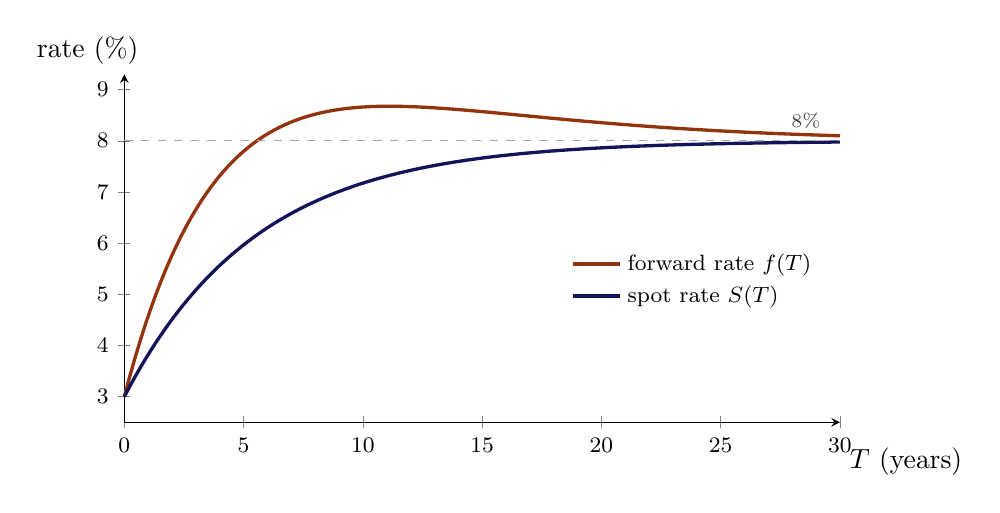
\begin{tikzpicture}
		\begin{axis}[
				width=0.88\textwidth, height=6.0cm,
				xmin=0, xmax=30, ymin=2.5, ymax=9.3,
				xtick={0,5,10,15,20,25,30},
				ytick={3,4,5,6,7,8,9},
				xlabel={$T$ (years)}, ylabel={rate (\%)},
				label style={font=\footnotesize, text=Gray!60!black},
				every axis y label/.style={at={(ticklabel cs:1.0)}, rotate=0, anchor=south},
				every axis x label/.style={at={(ticklabel cs:1.0)}, anchor=west},
				axis x line=bottom, axis y line=left,
				axis line style={thin},
				tick label style={font=\footnotesize},
				legend style={font=\footnotesize, at={(0.98,0.30)},
						anchor=south east, draw=none, fill=none},
				legend cell align=left,
				clip=false,
			]
			\addplot[RawSienna, very thick, domain=0:30, samples=140]
			{100*(0.08-0.05*exp(-0.18*x)+0.009*x*exp(-0.18*x))};
			\addlegendentry{forward rate $f(T)$}
			\addplot[MidnightBlue!80!black, very thick, domain=0:30, samples=140]
			{100*(0.08-0.05*exp(-0.18*x))};
			\addlegendentry{spot rate $S(T)$}
			\addplot[Gray!70, dashed, domain=0:30, samples=2] {8};
			\node[font=\scriptsize, text=Gray!60!black, anchor=south east]
			at (axis cs:29.6,8.05) {$8\%$};
		\end{axis}
	\end{tikzpicture}
	\caption{The Hull--White spot curve and the forward curve it implies. The
		spot curve rises monotonically to its asymptote of $8\%$; the forward curve
		overshoots it, peaking at $8.68\%$ near $T=11.1$ before falling back. Both
		start at $3\%$, since $f(0)=S(0)$.}
	\label{fig:hull-white}
\end{figure}

\begin{remark}
	遠期曲線\emph{衝過}長期水準再折返，這件事值得解釋——它不是畫錯了。

	$S(T)$ 是 $[0,T]$ 上所有瞬時利率的平均。
	既然平均要從 $3\%$ 一路爬到 $8\%$，而起點被壓在 $3\%$，那麼中段的瞬時利率就必須\emph{高於} $8\%$，才拉得動整條平均線。
	等到平均值接近 $8\%$、不再需要被拉動時，$f$ 才降回 $8\%$。

	這正是「邊際領先平均」的標準圖像，也是實務上常說的：\emph{遠期曲線是即期曲線的放大版}——即期曲線的任何斜率，在遠期曲線上都被乘上 $T$ 放大了（見 \eqref{eq:inst-fwd}）。
\end{remark}

%─────§ Term structure theories─────────────────────────────────────────────────────────────────────────────────────────────────────────────────────
\section{Term Structure Theories}
\label{sec:ts-theories}

Everything up to here was arithmetic: given prices, the forward rates follow by identity.
The remaining question is economic --- what, if anything, does $f(i,j)$ say about the \emph{future} spot rate $S(i,j)$?
Answering it requires an assumption, and the candidate assumptions are the term structure theories.

\subsection{Unbiased Expectations Theory}

\source{Slides p.~155}

\begin{theorem}[Unbiased expectations theory]
	The forward rate equals the average future spot rate,
	\begin{equation}
		f(a,b) \;=\; E\bigl[\,S(a,b)\,\bigr] . \label{eq:uet}
	\end{equation}
\end{theorem}

\begin{itemize}[nosep]
	\item It does \emph{not} imply that the forward rate is an accurate predictor for the future spot rate.
	\item It implies the maturity strategy and the rollover strategy produce the same result at the horizon ``on average''.
\end{itemize}

\begin{remark}
	先釐清定理本身：$f(a,b)$ 是今天就算得出來的數字，$S(a,b)$ 則要到時點 $a$ 才會在市場上報出來，今天看它是隨機變數。
	這個理論假設前者等於後者的期望值。它是一個關於市場的\emph{假設}，不是前面那種由無套利推出來的定理。

	\textbf{第一點：「無偏」不等於「準」。}
	$f(a,b)=E[S(a,b)]$ 只是說 forward rate 沒有\emph{系統性}地偏高或偏低：把很多次的預測誤差 $S(a,b)-f(a,b)$ 平均起來是 $0$。
	但任何一次實際報出的 $S(a,b)$ 都可能離 $f(a,b)$ 很遠，例如今天算出 $f(1,2)=5\%$，一年後的實際利率是 $3\%$ 或 $7\%$ 都跟理論不衝突。

	\textbf{第二點：兩種策略「平均」打平。}
	回想 \autoref{sec:forward-rates} 的兩種策略。
	maturity strategy 的終值今天已經確定；rollover strategy 的終值要用到未來的 $S(a,b)$，所以是隨機的。
	forward rate 的定義是：若 rollover 後半段的利率\emph{剛好}等於 $f(a,b)$，兩者就打平。
	這個理論再假設 $f(a,b)$ 是 $S(a,b)$ 的期望值，於是 rollover 的終值\emph{平均而言}等於 maturity 的終值；實際走出來的某一條路徑則可能高也可能低。
	「on average」加了引號，是因為這句話只在粗略意義下成立：終值裡的 $S(a,b)$ 是出現在 $(1+S(a,b))^{b-a}$ 裡，而一般來說 $E\bigl[(1+S)^{k}\bigr]\ne(1+E[S])^{k}$。
	下一小節的「bad」expectations theory 就是在這種細節上出問題。
\end{remark}

\source{Slides p.~156}

The theory ties the shape of today's curve to the market's expectations.

\begin{proposition}
	Under \eqref{eq:uet}, a normal spot rate curve is due to the fact that the market expects the future spot rate to rise.
	Conversely, the spot rate is expected to fall if and only if the spot rate curve is inverted.
\end{proposition}

\begin{proof}
	First, $f(j,j+1)>S(j+1)$ if and only if $S(j+1)>S(j)$.
	Indeed, by \eqref{eq:fwd-def},
	\[
		1+f(j,j+1) = \frac{\bigl(1+S(j+1)\bigr)^{j+1}}{\bigl(1+S(j)\bigr)^{j}} ,
	\]
	so $f(j,j+1)>S(j+1)$ is equivalent to $\bigl(1+S(j+1)\bigr)^{j}>\bigl(1+S(j)\bigr)^{j}$, i.e.\ to $S(j+1)>S(j)$.
	Substituting \eqref{eq:uet} gives
	\[
		E\bigl[\,S(j,j+1)\,\bigr] > S(j+1) > \cdots > S(1)
		\qquad\text{if and only if}\qquad
		S(j+1) > \cdots > S(1) . \qedhere
	\]
\end{proof}

\begin{remark}
	第一個小結論\emph{不需要}任何理論——它純粹是 \eqref{eq:fwd-def} 的代數重寫，也就是 \autoref{sec:fwd-vs-spot} 的特例。
	理論的作用只在最後一步：把算出來的 $f(j,j+1)$ 換成\emph{期望值} $E[S(j,j+1)]$。

	\textbf{那串不等式為什麼等於「預期利率上升」？}
	關鍵是把每個符號讀成「哪個時點的一期利率」：
	\begin{itemize}[nosep]
		\item $S(1)=S(0,1)$ 是\emph{今天}的一期利率；
		\item $S(j,j+1)$ 是\emph{時點 $j$} 的一期利率，今天未知，$E[S(j,j+1)]$ 就是市場對它的預期。
	\end{itemize}
	「預期未來利率上升」的意思就是：預期時點 $j$ 的一期利率高於今天的一期利率，即 $E[S(j,j+1)]>S(1)$。
	那串不等式的頭尾正是這件事：
	\[
		\underbrace{E\bigl[S(j,j+1)\bigr]}_{\text{預期的未來一期利率}}
		\;>\; S(j+1) \;>\; \cdots \;>\;
		\underbrace{S(1)}_{\text{今天的一期利率}} ,
	\]
	中間的 $S(j+1)>\cdots>S(1)$ 就是「spot curve 是 normal」。
	所以整句讀成：曲線 normal $\Longleftrightarrow$ 預期的未來一期利率高過今天的一期利率。

	直覺上：由 \eqref{eq:fwd-spot-prod}，$S(j+1)$ 是 $S(1),f(1,2),\ldots,f(j,j+1)$ 的（幾何）平均；在此理論下這些 $f$ 就是各期的\emph{預期}一期利率。
	所以長天期 spot rate 就是「今天的利率加上未來各期預期利率」的平均。
	平均值隨期限上升（normal），唯一的原因就是後面加進來的預期利率比較高——市場預期利率會漲。

	所以這條命題的內容其實是：\textbf{在}\vocab{無偏預期理論}（unbiased expectations theory）\textbf{之下}，「殖利率曲線正常」與「市場預期短率將上升」是同一件事。
	這也是新聞上「倒掛的殖利率曲線預示降息」那句話的理論根據——但別忘了它\emph{建立在假設之上}，而下一小節正是要說明這一類假設有多脆弱。
\end{remark}

\subsection{A ``Bad'' Expectations Theory}

\source{Slides p.~157}

Consider the natural-sounding strengthening: the expected returns\footnote{More precisely, the one-plus returns.} on all possible riskless bond strategies are equal for all holding periods.
It turns out to be internally inconsistent.

Over a \emph{two}-period horizon, buying a two-period bond and rolling over one-period bonds must tie:
\begin{equation}
	\bigl(1+S(2)\bigr)^{2} \;=\; \bigl(1+S(1)\bigr)\,E\bigl[\,1+S(1,2)\,\bigr] . \label{eq:bad-two}
\end{equation}
After rearrangement,
\begin{equation}
	\frac{1}{E\bigl[\,1+S(1,2)\,\bigr]} \;=\; \frac{1+S(1)}{\bigl(1+S(2)\bigr)^{2}} . \label{eq:bad-two-rearranged}
\end{equation}

\begin{remark}
	\textbf{這個理論在說什麼。}
	先固定一個\vocab{持有期間}（holding period）$H$：今天投入 \$1，看時點 $H$ 手上有多少。
	在這 $H$ 期內，用無違約風險的債券可以有很多玩法：買 $H$ 期 zero 持有到期、買短的一路 rollover、買更長的 zero 然後在時點 $H$ 提前賣掉……
	這個理論主張：\emph{只要持有期間相同}，所有這些策略的\emph{預期} one-plus return 都相等，而且這對\emph{每一個} $H$ 都成立。
	其中 \vocab{one-plus return} $=$ 期末價值 $/$ 期初投入，算的是\emph{整個持有期間}：例如兩期 zero 持有兩期是 $(1+S(2))^{2}$，不是 $1+S(2)$。

	背後的想法是：若投資人只看期望報酬、不在乎風險，那麼哪個策略的期望報酬比較高，大家就會去搶，價格被推到直到打平為止。
	注意「無風險」只是指不會違約；rollover 或提前賣出時，未來的利率與價格今天仍未知，所以報酬還是隨機的，才需要取期望值。

	\textbf{所以什麼時候「要相等」？}
	只比\emph{同一個持有期間}的策略：
	\begin{itemize}[nosep]
		\item $H=2$（這一頁）：兩期 zero 持有到期 vs.\ 一期 zero rollover 兩次；
		\item $H=1$（p.~158--159）：一期 zero 持有到期（報酬確定是 $1+S(1)$）vs.\ 兩期 zero 持有一期後賣掉（賣價未知）。
	\end{itemize}
	p.~159 說「the theory says the returns are equal」，就是因為那兩個策略的持有期間都是 $1$，理論要求它們預期報酬相同。

	\textbf{跟 unbiased expectations theory 的關係。}
	不是先相信 unbiased expectations theory 再去推廣它。
	單看 $H=2$ 那條式子，它其實就是 unbiased expectations theory 用在 $f(1,2)$ 上（$E[S(1,2)]=f(1,2)$）；單看 $H=1$ 那條式子，它就是下一小節的 local expectations theory。
	兩條\emph{各自}都可以成立，這個「bad」theory 的問題是把「投資人不在乎風險」這個直覺\emph{同時}套到所有持有期間上。
	接下來三頁要證明：兩條式子不可能同時成立，除非未來利率毫無不確定性。
	所以結論不是「unbiased expectations theory 錯了」，而是「expectations theory 只能挑一個持有期間來要求，不能全都要」。

	\textbf{證明的策略。}
	先用 $H=2$ 得到一條等式（這一頁），再用 $H=1$ 得到另一條（下一頁），兩條合起來會跟 Jensen's inequality 衝突。

	\textbf{兩期的持有期間。}
	今天投入 \$1，看時點 $2$ 的結果：
	\begin{itemize}[nosep]
		\item 買兩期 zero 持有到期：終值 $(1+S(2))^{2}$，今天就確定；
		\item 買一期 zero，時點 $1$ 再以當時的利率 $S(1,2)$ 滾一期：終值 $(1+S(1))(1+S(1,2))$，因為 $S(1,2)$ 今天未知，只能取期望值。
	\end{itemize}
	理論說兩者預期相等，就是 \eqref{eq:bad-two}。
	到這裡還只是 unbiased expectations theory 的兩期版本（$E[1+S(1,2)]=1+E[S(1,2)]$），沒有任何問題。
\end{remark}

\source{Slides p.~158}

Now consider two \emph{one}-period strategies.

\begin{itemize}[nosep]
	\item Strategy one buys a two-period bond for $(1+S(2))^{-2}$ dollars and sells it after one period.
	      Its price then will be $(1+S(1,2))^{-1}$, so the expected return is
	      \[
		      E\bigl[\,(1+S(1,2))^{-1}\,\bigr]\big/(1+S(2))^{-2} .
	      \]
	\item Strategy two buys a one-period bond with a return of $1+S(1)$.
\end{itemize}

\source{Slides p.~159}

The theory says the returns are equal:
\[
	\frac{1+S(1)}{\bigl(1+S(2)\bigr)^{2}} \;=\; E\left[\frac{1}{1+S(1,2)}\right] .
\]
Combining this with \eqref{eq:bad-two-rearranged} yields
\begin{equation}
	E\left[\frac{1}{1+S(1,2)}\right] \;=\; \frac{1}{E\bigl[\,1+S(1,2)\,\bigr]} . \label{eq:bad-clash}
\end{equation}

\source{Slides p.~160}

\begin{proposition}
	\eqref{eq:bad-clash} is impossible save for a certain economy --- that is, unless $S(1,2)$ is known today.
	（除非是一個\emph{確定性}的經濟——也就是未來利率 $S(1,2)$ 今天就已知、沒有任何隨機性——否則 \eqref{eq:bad-clash} 不可能成立。這裡的 save for 是「除了」。）
\end{proposition}

\begin{proof}
	Jensen's inequality states that $E[\,g(X)\,]>g\bigl(E[X]\bigr)$ for any nondegenerate random variable $X$ and strictly convex function $g$ (i.e.\ $g''(x)>0$).
	Use
	\[
		g(x) \;\triangleq\; (1+x)^{-1} ,
	\]
	for which $g''(x)=2(1+x)^{-3}>0$ whenever $x>-1$.
	With $X=S(1,2)$,
	\[
		E\left[\frac{1}{1+S(1,2)}\right] \;>\; \frac{1}{1+E[\,S(1,2)\,]} \;=\; \frac{1}{E[\,1+S(1,2)\,]} ,
	\]
	which contradicts \eqref{eq:bad-clash} unless $S(1,2)$ is degenerate, i.e.\ deterministic.
\end{proof}

\begin{remark}
	這個結果的教訓比它的算式重要，值得講清楚。

	\textbf{錯在哪裡？}不在於某一個式子算錯，而在於這個理論\emph{要求太多}：它同時宣稱所有期間長度、所有策略的期望報酬都相等。
	兩期視角給出 \eqref{eq:bad-two}，一期視角給出另一條式子，兩者合起來就逼出 \eqref{eq:bad-clash}——一個只有在未來利率\emph{毫無不確定性}時才成立的等式。

	\textbf{根源是「期望值」與「取倒數」不可交換。}
	債券價格是利率的凸函數（$1/(1+x)$ 凸），所以「先取期望再折現」與「先折現再取期望」必然不同，差額就是 \vocab{Jensen 不等式}（Jensen's inequality）留下的缺口。
	這與 \autoref{sec:convexity} 的凸性其實是同一件事的兩個面貌：那裡凸性讓持有人「漲賺得比跌賠得多」，這裡凸性讓 $E[1/(1+X)] > 1/E[1+X]$。

	\textbf{出路}是只挑\emph{一種}視角來要求，別全都要——這就是下一小節的\vocab{局部預期理論}（local expectations theory）。
\end{remark}

\subsection{Local Expectations Theory}

\source{Slides p.~161}

\begin{theorem}[Local expectations theory]
	The expected rate of return of any bond over \emph{a single period} equals the prevailing one-period spot rate:
	\begin{equation}
		\frac{E\bigl[\,(1+S(1,n))^{-(n-1)}\,\bigr]}{(1+S(n))^{-n}} \;=\; 1+S(1)
		\qquad \text{for \emph{all} } n>1 . \label{eq:let}
	\end{equation}
\end{theorem}

\begin{remark}
	\eqref{eq:let} 就是「今天買一張 $n$ 期 zero、持有\emph{一期}後賣掉」的預期 one-plus return（賣價 $/$ 買價）：
	\begin{itemize}[nosep]
		\item 分母 $(1+S(n))^{-n}$：這張 $n$ 期 zero 今天的價格（買價）；
		\item 分子：到了時點 $1$，它變成剩 $n-1$ 期的 zero，當時的價格是 $(1+S(1,n))^{-(n-1)}$，其中 $S(1,n)$ 是時點 $1$ 才報出的利率，今天未知，所以取期望值（預期賣價）；
		\item 右邊 $1+S(1)$：直接買一期 zero 持有到期的報酬，今天就確定。
	\end{itemize}
	兩邊比的是\emph{比值}，與買多少無關：左邊用面額 \$1 的 zero 算，右邊若也用面額 \$1 的一期 zero，買價 $(1+S(1))^{-1}$、到期拿 \$1，比值同樣是 $1+S(1)$，跟「投入 \$1 拿回 $1+S(1)$」一樣。
	所以整條式子說：\emph{持有一期的話，買哪一張 zero 預期報酬都一樣，都等於一期利率}。
	$n=2$ 就是 p.~159 那條式子；這裡只要求持有期間 $H=1$，不再同時要求 $H=2$，因此不會碰到上一小節的 Jensen 矛盾。

	等價的寫法是把分母移過去：
	\[
		\underbrace{(1+S(n))^{-n}}_{\text{今天價格}} \;=\; \frac{E\bigl[\,\text{時點 } 1 \text{ 的價格}\,\bigr]}{1+S(1)} ,
	\]
	即今天的價格 $=$ 下一期的預期價格用一期利率折現回來。(today's price of every bond is the expectation of its price next period, discounted at the known one-period rate. 	That is precisely the recursive structure a tree or lattice model needs, which is why the theory reappears later in the course as the \emph{risk-neutral} pricing convention.)
\end{remark}

%─────§ Duration in practice────────────────────────────────────────────────────────────────────────────────────────────────────────────────────────
\section{Duration, in Practice}
\label{sec:duration-practice}

\source{Slides p.~162}

We had assumed parallel shifts in the spot rate curve --- the caveat flagged back in \autoref{sec:portfolio-duration}.
Now that the curve is a genuine object with $n$ separate coordinates, that assumption can be relaxed.

To handle more general shifts, define a vector $[\,c_{1},c_{2},\ldots,c_{n}\,]$ that characterizes the shift:

\begin{itemize}[nosep]
	\item Parallel shift: $[\,1,1,\ldots,1\,]$.
	\item Twist: $[\,1,1,\ldots,1,-1,\ldots,-1\,]$, $[\,1.8,1.6,1.4,1,0,-1,-1.4,\ldots\,]$, etc.
	\item \ldots
\end{itemize}

At least one $c_{i}$ should be $1$ as the reference point.

\begin{figure}[H]
	\centering
	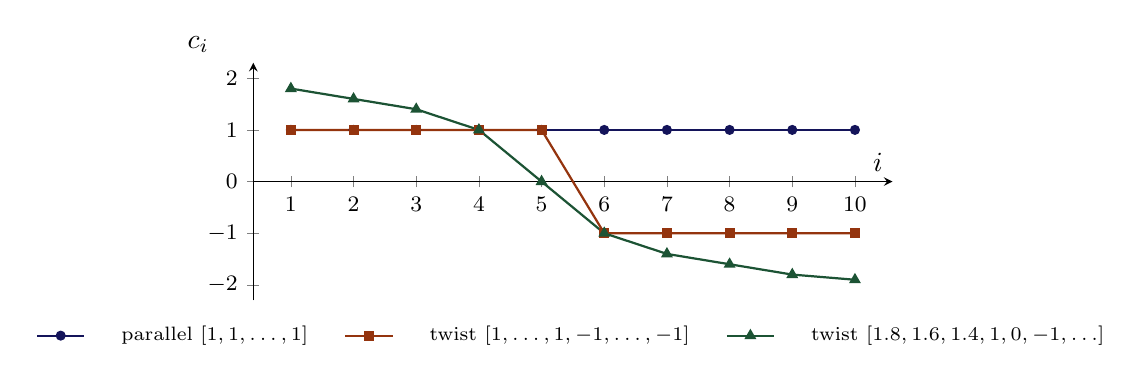
\begin{tikzpicture}
		\begin{axis}[
				width=0.80\textwidth, height=4.6cm,
				xmin=0.4, xmax=10.6, ymin=-2.3, ymax=2.3,
				xtick={1,2,3,4,5,6,7,8,9,10},
				ytick={-2,-1,0,1,2},
				xlabel={$i$}, ylabel={$c_{i}$},
				label style={font=\footnotesize, text=Gray!60!black},
				every axis y label/.style={at={(ticklabel cs:1.0)}, rotate=0, anchor=south},
				every axis x label/.style={at={(ticklabel cs:1.0)}, anchor=west},
				axis x line=middle, axis y line=left,
				axis line style={thin},
				tick label style={font=\footnotesize},
				legend style={font=\scriptsize, at={(0.5,-0.06)},
						anchor=north, draw=none, fill=none,
						legend columns=3, column sep=1.1em},
				legend cell align=left,
				clip=false,
			]
			\addplot[MidnightBlue!80!black, thick, mark=*, mark size=1.4pt]
			coordinates {(1,1) (2,1) (3,1) (4,1) (5,1) (6,1) (7,1) (8,1) (9,1) (10,1)};
			\addlegendentry{parallel $[1,1,\dots,1]$}
			\addplot[RawSienna, thick, mark=square*, mark size=1.4pt]
			coordinates {(1,1) (2,1) (3,1) (4,1) (5,1) (6,-1) (7,-1) (8,-1) (9,-1) (10,-1)};
			\addlegendentry{twist $[1,\dots,1,-1,\dots,-1]$}
			\addplot[SeaGreen!60!black, thick, mark=triangle*, mark size=1.7pt]
			coordinates {(1,1.8) (2,1.6) (3,1.4) (4,1) (5,0) (6,-1) (7,-1.4)
					(8,-1.6) (9,-1.8) (10,-1.9)};
			\addlegendentry{twist $[1.8,1.6,1.4,1,0,-1,\dots]$}
		\end{axis}
	\end{tikzpicture}
	\caption{Shift vectors. Each describes how much the spot rate at maturity
		$i$ moves per unit of the common factor $y$; a parallel shift is the special
		case in which every maturity moves alike.}
	\label{fig:shift-vectors}
\end{figure}

\begin{remark}
	\textbf{問題在哪。}
	之前算 duration 時說「利率上升 $\Delta y$，價格掉多少」，暗中假設曲線上\emph{每一期}的 spot rate 都一起上升 $\Delta y$，也就是整條曲線平移（parallel shift）。
	但實際上曲線常常不是這樣動的：可能短天期漲、長天期跌（曲線變平或倒掛），也可能中間動得多、兩端動得少。

	\textbf{這一頁的做法。}
	把「曲線怎麼動」拆成兩部分：
	\[
		S(i) \;\longrightarrow\; S(i) + y\,c_{i} ,
	\]
	\begin{itemize}[nosep]
		\item $y$：一個數字，代表\emph{動多大}；
		\item $[c_{1},\ldots,c_{n}]$：一個向量，代表\emph{動的形狀}——第 $i$ 期跟著 $y$ 動幾倍。
	\end{itemize}
	以 $y=0.1\%$ 為例：
	\begin{itemize}[nosep]
		\item $[1,1,\ldots,1]$：每一期都 $+0.1\%$，就是原本的平移；
		\item $[1,\ldots,1,-1,\ldots,-1]$：前幾期 $+0.1\%$、後幾期 $-0.1\%$，短端漲長端跌，曲線被「扭」了（twist）；
		\item $[1.8,1.6,1.4,1,0,-1,\ldots]$：第 $1$ 期 $+0.18\%$、第 $4$ 期 $+0.1\%$、第 $5$ 期不動、再往後轉為下跌，是比較平滑的扭轉。
	\end{itemize}
	上圖就是把這三個向量畫出來：橫軸是期別 $i$，縱軸是 $c_{i}$。

	\textbf{為什麼要有一個 $c_{i}=1$。}
	$y$ 和 $c_{i}$ 只以乘積出現，$[c_{i}]$ 全部乘 $2$、$y$ 除以 $2$ 是同一種變動，所以要固定尺度。
	規定某一期的 $c_{i}=1$，$y$ 就有了明確意義：\emph{那一期}的 spot rate 動了多少。

	下一頁再用這個 $y$ 定義 duration：$y$ 動一點點時，價格變動的百分比。
	它是原本 duration 的推廣：若形狀選平移 $[1,\ldots,1]$、\emph{且}曲線本來就是平的（$S(i)$ 全等於某個 $r$），價格變成 $P(y)=\sum_{i} C_{i}/(1+r+y)^{i}$，這正是把殖利率從 $r$ 移到 $r+y$ 的價格函數，
	於是 $-\dfrac{1}{P}\dfrac{\partial P}{\partial y}\Big|_{y=0}=\dfrac{1}{P}\sum_{i}\dfrac{i\,C_{i}}{(1+r)^{i+1}}$，恰好就是 \eqref{eq:mod-dur} 的 modified duration。
\end{remark}

\source{Slides p.~163}

\begin{definition}[Duration under a general shift]
	Let
	\begin{equation}
		P(y) \;\triangleq\; \sum_{i} \frac{C_{i}}{\bigl(1+S(i)+y\,c_{i}\bigr)^{i}} \label{eq:dur-shift}
	\end{equation}
	be the price associated with the cash flow $C_{1},C_{2},\ldots$, and define duration as
	\[
		-\left.\frac{\partial P(y)/P(0)}{\partial y}\right|_{y=0}
		\qquad\text{or}\qquad
		-\,\frac{P(\Delta y)-P(-\Delta y)}{2P(0)\,\Delta y} .
	\]
\end{definition}

Modified duration equals the above when
\[
	[\,c_{1},c_{2},\ldots,c_{n}\,] = [\,1,1,\ldots,1\,] ,
	\qquad
	S(1)=S(2)=\cdots=S(n) .
\]

\begin{remark}
	這一節把第三章的 duration 放回正確的位置，值得把三件事對齊。

	\textbf{（一）$y$ 換了角色。}
	\eqref{eq:dur-shift} 裡的 $y$ 不再是殖利率，而是一個\emph{抽象的衝擊大小}；真正決定各期利率怎麼動的是向量 $[c_{i}]$。
	$y$ 動一單位，第 $i$ 期的即期利率就動 $c_{i}$ 單位。

	\textbf{（二）為什麼要有「至少一個 $c_{i}=1$」。}
	$y$ 與 $[c_{i}]$ 只以乘積 $y c_{i}$ 出現，把 $[c_{i}]$ 全部乘以 $2$、$y$ 全部除以 $2$，模型完全一樣。
	固定某個 $c_{i}=1$ 就是挑一個\emph{參考期別}來定尺度，讓算出來的 duration 有明確的單位：「當那一期的利率動 $1$ 時，價格動幾個百分比」。

	\textbf{（三）第二個公式就是中央差分。}
	它與 \eqref{eq:eff-dur} 的 effective duration 是同一個數值技巧，只是這裡擾動的是整條曲線而非單一殖利率——連同 \autoref{sec:eff-conv} 之後那段關於 $\Delta y$ 取多大的討論，也照樣適用。

	實務上把不同的 $[c_{i}]$ 各算一個 duration，就得到\vocab{關鍵利率存續期間}（key rate duration）：取 $[c_{i}]$ 為只在某一期為 $1$、其餘為 $0$ 的向量，便可量出部位對曲線上\emph{各個點}的個別暴險，而不是只有一個總數。
	一個 duration 為零的部位，仍可能對\vocab{扭轉}（twist）有巨大暴險。
	twist 指曲線繞著某個期別「轉動」：一端上升、另一端下降，改變的是曲線的\emph{斜率}而不是整體高低（例如短端 $-0.1\%$、長端 $+0.1\%$，曲線變陡）。
	例如持有長天期債券、同時放空短天期債券，把數量配到平移下的 duration 為零；平移時兩邊損益互相抵銷，但遇到上述變陡的 twist，長債因長端利率上升而跌價、放空的短債因短端利率下降而漲價，兩邊\emph{同時}虧錢。
\end{remark}

%─────§ Loose ends─────────────────────────────────────────────────────────────────────────────────────────────────────────────────────────────────
\section{Some Loose Ends on Dates}

\source{Slides p.~164}

Every formula in this chapter has indexed time by integers $1,2,\ldots,n$.
Converting those to actual dates raises a list of unglamorous questions that nonetheless have to be answered before any of it can be coded:

\begin{itemize}[nosep]
	\item Holidays.
	\item Weekends.
	\item Business days ($T+2$, etc.).
	\item Shall we treat a year as $1$ year whether it has $365$ or $366$ days?
\end{itemize}

\begin{note}
	These are the same concerns as the day count conventions of \autoref{sec:day-count}, now compounded by the settlement calendar.
	None of them is deep, and all of them are mandatory: a discount factor $d(i)$ is only as well defined as the date $i$ names, and two desks using different holiday calendars will bootstrap two different curves from the same quotes.

	（翻譯：這些問題和 \autoref{sec:day-count} 的 day count convention 是同一類，只是現在還多疊了一層\vocab{交割日曆}（settlement calendar）的問題。
	它們都不深奧，卻\emph{每一個都非處理不可}：折現因子 $d(i)$ 的定義只能跟「第 $i$ 期」指的是哪一天一樣明確；
	兩個交易櫃檯若用不同的假日日曆，拿同一組報價 bootstrap 出來的曲線就會不同。
	其中 $T+2$ 指成交後第 $2$ 個營業日才交割（錢券互換），所以現金流的實際日期還要跳過週末與假日來算。）
\end{note}

%─────Fundamental Statistical Concepts───────────────────────────────────────────────────────────────────────────────────────────────────────────────
\chapter{Fundamental Statistical Concepts}

\source{Slides pp.~165--166}

\begin{flushright}
	\itshape There are three kinds of lies:\\
	lies, damn lies, and statistics.\\
	\upshape --- Misattributed to Benjamin Disraeli (1804--1881)

	\medskip

	\itshape If 50 million people believe a foolish thing,\\
	it's still a foolish thing.\\
	\upshape --- George Bernard Shaw (1856--1950)

	\medskip

	\itshape One death is a tragedy,\\
	but a million deaths are a statistic.\\
	\upshape --- Josef Stalin (1879--1953)
\end{flushright}

\bigskip

\noindent Everything so far has been deterministic.
A bond's cash flows were known, the curve was observed, and the only uncertainty admitted --- in the term structure theories of \autoref{sec:ts-theories} --- was smuggled in through an expectation operator that was never defined.

This chapter supplies the vocabulary that the rest of the course runs on.
Nothing in it is deep; what matters is that every later model, from the binomial tree to Black--Scholes to Monte Carlo pricing, is assembled from these pieces.
Three of them will do most of the work:

\begin{itemize}[nosep]
	\item \textbf{Conditional expectation}, which is how a model says ``given what we know today''.
	\item \textbf{The normal distribution}, which is what we will assume \emph{log} returns follow.
	\item \textbf{The lognormal distribution}, which is what prices then follow --- and the reason \eqref{eq:lognormal-partial} below turns into the Black--Scholes formula later on.
\end{itemize}

\begin{note}
	The epigraphs are a warning worth keeping.
	\autoref{fig:sp500-density} already showed that real returns are \emph{not} normal: the tails are far too heavy.
	We use the normal distribution anyway, because it is the only one that stays tractable under the operations we need.
	The discipline recommended by the Modelers' Hippocratic Oath in \autoref{sec:oath} applies exactly here --- know precisely where the assumption is wrong.
\end{note}

%─────§ Moments────────────────────────────────────────────────────────────────────────────────────────────────────────────────────────────────────
\section{Moments}

\source{Slides p.~167}

\begin{definition}
	The \vocab{variance} of a random variable $X$ is defined as
	\begin{equation}
		\Var[\,X\,] \;\triangleq\; E\bigl[\,(X-E[\,X\,])^{2}\,\bigr] . \label{eq:variance}
	\end{equation}
	The \vocab{covariance} between random variables $X$ and $Y$ is
	\begin{equation}
		\Cov[\,X,Y\,] \;\triangleq\; E\bigl[\,(X-\mu_{X})(Y-\mu_{Y})\,\bigr] , \label{eq:covariance}
	\end{equation}
	where $\mu_{X}$ and $\mu_{Y}$ are the means of $X$ and $Y$, respectively.
	Random variables $X$ and $Y$ are \vocab{uncorrelated} if $\Cov[\,X,Y\,]=0$.
\end{definition}

Expanding the products gives the computational forms used in practice,
\[
	\Var[\,X\,] = E[\,X^{2}\,]-\bigl(E[\,X\,]\bigr)^{2} ,
	\qquad
	\Cov[\,X,Y\,] = E[\,XY\,]-E[\,X\,]E[\,Y\,] ,
\]
and taking $Y=X$ in \eqref{eq:covariance} recovers $\Cov[\,X,X\,]=\Var[\,X\,]$: variance is covariance with oneself.

\begin{remark}
	\vocab{不相關}（uncorrelated）\textbf{ $\neq$ }\vocab{獨立}（independent）\textbf{，這是本章最容易出錯的地方。}

	獨立是說「$X$ 的任何資訊都不告訴你 $Y$ 的任何事」；不相關只是說\emph{線性}關係為零。
	獨立必然不相關，反之不然。

	標準反例：取 $X\sim N(0,1)$，$Y=X^{2}$。
	此時 $\Cov[X,Y]=E[X^{3}]-E[X]E[X^{2}]=0-0=0$，兩者不相關；但 $Y$ 完全由 $X$ 決定，談不上獨立。

	為什麼在金融裡特別要緊？
	因為風險管理常以「相關係數低」來論證分散效果，而危機時真正咬人的往往是\emph{非線性}的相依——平時各走各的，一起崩盤時卻同時跌。
	相關係數對這種結構是盲的。
\end{remark}

%─────§ Correlation────────────────────────────────────────────────────────────────────────────────────────────────────────────────────────────────
\section{Correlation}

\source{Slides p.~168}

\begin{definition}
	The \vocab{standard deviation} of $X$ is the square root of the variance,
	\[
		\sigma_{X} \;\triangleq\; \sqrt{\Var[\,X\,]} .
	\]
	The \vocab{correlation} (or \vocab{correlation coefficient}) between $X$ and $Y$ is
	\begin{equation}
		\rho_{X,Y} \;\triangleq\; \frac{\Cov[\,X,Y\,]}{\sigma_{X}\sigma_{Y}} , \label{eq:correlation}
	\end{equation}
	provided both have nonzero standard deviations.\footnote{Wilmott (2009): ``the correlations between financial quantities are notoriously unstable.'' It may even break down ``at high-frequency time intervals'' (Budish, Cramton, \& Shim, 2015).}
\end{definition}

\begin{note}
	Dividing by $\sigma_{X}\sigma_{Y}$ makes $\rho$ dimensionless and confines it to $[-1,1]$, by the Cauchy--Schwarz inequality
	$\bigl|\Cov[X,Y]\bigr|\le\sigma_{X}\sigma_{Y}$, with equality exactly when $Y$ is an affine function of $X$.
	Covariance says how two variables co-move \emph{and} how big they are; correlation strips out the size.
\end{note}

\begin{remark}
	那個腳註不是客套話，值得展開。

	\textbf{（一）相關係數不穩定。}
	$\rho$ 是用歷史樣本估出來的，而它本身會隨時間漂移——尤其在市場承壓時往往整體跳向 $1$。
	用平時估出來的 $\rho$ 去計算危機時的投資組合風險，會系統性地低估損失；2008 年的結構型商品定價正是栽在這裡。

	\textbf{（二）高頻下會崩解。}
	把觀測間隔縮短到毫秒等級，兩個本來高度相關的資產（例如 S\&P 500 期貨與其 ETF）算出來的相關係數會急遽下降——這就是所謂的 \vocab{Epps 效應}（Epps effect）。
	原因是兩邊的成交並非同時發生，取樣間隔一短，非同步性造成的雜訊就蓋過真正的共同波動。
	Budish、Cramton 與 Shim（2015）指出，這個在極短時間尺度上反覆出現的價差，正是高頻交易「軍備競賽」的獵物。

	\textbf{結論：}$\rho$ 是一個\emph{取樣間隔與樣本期間的函數}，報告時必須說清楚是用什麼頻率、什麼期間算的。
\end{remark}

%─────§ Variance of sum────────────────────────────────────────────────────────────────────────────────────────────────────────────────────────────
\section{Variance of a Sum}

\source{Slides p.~169}

\begin{proposition}
	The variance of a weighted sum of random variables equals
	\begin{equation}
		\Var\left[\,\sum_{i=1}^{n} a_{i}X_{i}\,\right]
		\;=\; \sum_{i=1}^{n}\sum_{j=1}^{n} a_{i}a_{j}\,\Cov[\,X_{i},X_{j}\,] . \label{eq:var-sum}
	\end{equation}
	It becomes
	\begin{equation}
		\sum_{i=1}^{n} a_{i}^{2}\,\Var[\,X_{i}\,] \label{eq:var-sum-uncorr}
	\end{equation}
	when the $X_{i}$ are uncorrelated.\footnote{Bienaym\'e (1853).}
\end{proposition}

\begin{proof}
	Write $Z=\sum_{i}a_{i}(X_{i}-\mu_{i})$, so that $E[Z]=0$ and $\Var[\sum_i a_i X_i]=E[Z^{2}]$. Then
	\[
		E[Z^{2}] = E\left[\sum_{i}\sum_{j} a_{i}a_{j}(X_{i}-\mu_{i})(X_{j}-\mu_{j})\right]
		= \sum_{i}\sum_{j} a_{i}a_{j}\,\Cov[\,X_{i},X_{j}\,]
	\]
	by linearity of expectation.
	If the $X_{i}$ are uncorrelated, every off-diagonal term vanishes and only the $i=j$ terms, $a_{i}^{2}\Var[X_{i}]$, survive.
\end{proof}

\begin{intuition}
	\eqref{eq:var-sum-uncorr} is the arithmetic of diversification.
	Hold $n$ uncorrelated assets in equal weights $a_{i}=1/n$, each with variance $\sigma^{2}$; the portfolio variance is $n\cdot(1/n)^{2}\sigma^{2}=\sigma^{2}/n$, which vanishes as $n$ grows.
	Correlation is what stops this: in \eqref{eq:var-sum} the $n^{2}-n$ off-diagonal terms outnumber the $n$ diagonal ones, so for large $n$ the portfolio variance is governed almost entirely by the \emph{average covariance}, not by the individual variances.

	\vocab{分散投資}（diversification）之所以有效，是因為 \eqref{eq:var-sum-uncorr} 的 $\sigma^{2}/n$ 會隨 $n$ 趨近於零。
	真正的限制在 \eqref{eq:var-sum}：非對角項有 $n^{2}-n$ 個，對角項只有 $n$ 個，$n$ 一大，組合的變異數幾乎完全由\emph{平均共變異數}決定——分散得掉個別風險，分散不掉共同風險。
\end{intuition}

%─────§ Conditional expectation─────────────────────────────────────────────────────────────────────────────────────────────────────────────────────
\section{Conditional Expectation}

\source{Slides p.~170}

\begin{definition}
	``$X\mid I$'' denotes $X$ conditional on the information set $I$; the information set can be another random variable's value, or the past values of $X$, say.
	The \vocab{conditional expectation}
	\[
		E[\,X\mid I\,]
	\]
	is the expected value of $X$ conditional on $I$.
	It is itself a \emph{random variable}.
\end{definition}

\begin{theorem}[Law of iterated conditional expectations, or the tower law]
	\begin{equation}
		E[\,X\,] \;=\; E\bigl[\,E[\,X\mid I\,]\,\bigr] . \label{eq:tower}
	\end{equation}
\end{theorem}

\source{Slides p.~171}

\begin{theorem}
	If $I_{2}$ contains at least as much information as $I_{1}$, then
	\begin{equation}
		E[\,X\mid I_{1}\,] \;=\; E\bigl[\,E[\,X\mid I_{2}\,]\mid I_{1}\,\bigr] . \label{eq:tower-nested}
	\end{equation}
\end{theorem}

Here $I_{1}$ contains price information up to time $t_{1}$, and $I_{2}$ contains price information up to a later time $t_{2}>t_{1}$.
In general,
\[
	I_{1}\subseteq I_{2}\subseteq\cdots
\]
means the players never forget past data, so the information sets are increasing over time.\footnote{Hirsa \& Neftci (2014). This idea is formalised by sigma fields and filtrations in probability theory.}

\begin{remark}
	這一節看起來抽象，但它是後面所有定價模型的語法，值得把三件事講清楚。

	\textbf{（一）為什麼 $E[X\mid I]$ 是隨機變數？}
	因為 $I$ 本身是隨機的。
	明天的股價期望值取決於今天觀察到什麼；今天的觀察結果尚未實現時，這個「期望值」就還是個變數。
	一旦 $I$ 實現了，它才塌縮成一個數字。

	\textbf{（二）\eqref{eq:tower-nested} 在講什麼？}
	用白話說：\emph{今天對「明天的預測」所做的預測，就是今天的預測}。
	你不可能今天就知道明天會把預測往上修——若知道，今天就該先修了。
	這正是\vocab{鞅}（martingale）的核心性質，也是無套利定價的技術支柱。

	\textbf{（三）$I_{1}\subseteq I_{2}\subseteq\cdots$ 為何要特別寫出來？}
	它把「資訊只增不減」這個看似當然的假設明白化。
	數學上這叫\vocab{過濾}（filtration），是隨機過程定義「時間」的方式——沒有它，「今天知道什麼」根本無從談起。
\end{remark}

%─────§ Normal distribution─────────────────────────────────────────────────────────────────────────────────────────────────────────────────────────
\section{The Normal Distribution}

\source{Slides p.~172}

\begin{definition}
	A random variable $X$ has the \vocab{normal distribution} with mean $\mu$ and variance $\sigma^{2}$ if its probability density function is
	\begin{equation}
		\frac{1}{\sigma\sqrt{2\pi}}\,e^{-(x-\mu)^{2}/(2\sigma^{2})} . \label{eq:normal-pdf}
	\end{equation}
	This is expressed by $X\sim N(\mu,\sigma^{2})$.
	The \vocab{standard normal distribution} has zero mean, unit variance, and the following distribution function:
	\begin{equation}
		\mathrm{Prob}[\,X\le z\,] \;\triangleq\; N(z) \;=\; \frac{1}{\sqrt{2\pi}}\int_{-\infty}^{z} e^{-x^{2}/2}\,dx . \label{eq:normal-cdf}
	\end{equation}
\end{definition}

\begin{note}
	The integral in \eqref{eq:normal-cdf} has no closed form in elementary functions, so $N(\cdot)$ is always evaluated numerically.
	Every option pricing formula in this course will end up calling it, which makes a fast and accurate $N(\cdot)$ a genuine implementation concern rather than a detail.
\end{note}

%─────§ MGF───────────────────────────────────────────────────────────────────────────────────────────────────────────────────────────────────────
\section{Moment Generating Functions}

\source{Slides p.~173}

\begin{definition}
	The \vocab{moment generating function} of a random variable $X$ is defined as
	\[
		\theta_{X}(t) \;\triangleq\; E\bigl[\,e^{tX}\,\bigr] .
	\]
\end{definition}

\begin{theorem}
	The moment generating function of $X\sim N(\mu,\sigma^{2})$ is
	\begin{equation}
		\theta_{X}(t) \;=\; \exp\left(\mu t + \frac{\sigma^{2}t^{2}}{2}\right) . \label{eq:normal-mgf}
	\end{equation}
\end{theorem}

\begin{remark}
	\textbf{為什麼叫}\vocab{動差生成函數}（moment generating function）\textbf{？}
	把 $e^{tX}$ 展開成 $\sum_{n\ge 0} t^{n}X^{n}/n!$ 再取期望值，得
	\[
		\theta_{X}(t) = \sum_{n\ge 0}\frac{E[\,X^{n}\,]}{n!}\,t^{n} ,
	\]
	所以 $\theta_{X}^{(n)}(0)=E[X^{n}]$——所有動差都藏在這一個函數裡，微分幾次就掉出第幾階動差。

	\textbf{為什麼現在就要提？}
	因為 \eqref{eq:normal-mgf} 在 $t=1$ 的值
	\[
		\theta_{X}(1) = E\bigl[\,e^{X}\,\bigr] = e^{\mu+\sigma^{2}/2}
	\]
	正是下一節對數常態分佈的平均數 \eqref{eq:lognormal-moments}。
	更一般地取 $t=n$ 就得到 $E[e^{nX}]=e^{n\mu+n^{2}\sigma^{2}/2}$，也就是 $E[Y^{n}]$——本章最後那一串對數常態公式，全部是 \eqref{eq:normal-mgf} 換個寫法而已。
\end{remark}

%─────§ Multivariate normal─────────────────────────────────────────────────────────────────────────────────────────────────────────────────────────
\section{The Multivariate Normal Distribution}

\source{Slides p.~174}

If $X_{i}\sim N(\mu_{i},\sigma_{i}^{2})$ are independent, then
\[
	\sum_{i} X_{i} \;\sim\; N\left(\sum_{i}\mu_{i},\;\sum_{i}\sigma_{i}^{2}\right) .
\]

Dropping independence requires a definition rather than a theorem.
Let $X_{i}\sim N(\mu_{i},\sigma_{i}^{2})$, which may not be independent, and suppose
\begin{equation}
	\sum_{i=1}^{n} t_{i}X_{i} \;\sim\;
	N\left(\sum_{i=1}^{n} t_{i}\mu_{i},\;
	\sum_{i=1}^{n}\sum_{j=1}^{n} t_{i}t_{j}\,\Cov[\,X_{i},X_{j}\,]\right) \label{eq:mvn-def}
\end{equation}
for every linear combination $\sum_{i=1}^{n}t_{i}X_{i}$ with $\sum_{i=1}^{n}\sum_{j=1}^{n}t_{i}t_{j}\Cov[\,X_{i},X_{j}\,]\neq 0$.

\source{Slides p.~175}

Then the $X_{i}$ are said to have a \vocab{multivariate normal distribution}.\footnote{Corrected by Mr.~Huang, Guo-Hua (\texttt{R98922107}) on March 10, 2010.}
With $M\equiv C^{-1}$ and the $(i,j)$th entry of the matrix $M$ being $M_{i,j}$, the probability density function for the $X_{i}$ is
\begin{equation}
	\frac{1}{\sqrt{(2\pi)^{n}\det(C)}}\,
	\exp\left[-\frac{1}{2}\sum_{i=1}^{n}\sum_{j=1}^{n}(X_{i}-\mu_{i})\,M_{ij}\,(X_{j}-\mu_{j})\right] , \label{eq:mvn-pdf}
\end{equation}
with a positive definite covariance matrix
\[
	C \;\triangleq\; \bigl[\,\Cov[\,X_{i},X_{j}\,]\,\bigr]_{1\le i,j\le n} .
\]

\begin{remark}
	\eqref{eq:mvn-def} 的定義方式初看奇怪——為什麼不直接寫聯合密度函數，卻繞道去要求「每一個線性組合都是常態」？

	理由是這個定義\emph{更廣也更好用}。
	密度函數 \eqref{eq:mvn-pdf} 需要 $C$ 可逆；若某些 $X_{i}$ 之間有完全線性相依（例如 $X_{3}=X_{1}+X_{2}$），$C$ 就退化、密度不存在，但 \eqref{eq:mvn-def} 依然成立。
	投影片上那個 $\neq 0$ 的但書正是在排除退化的線性組合。

	更實際的理由是：金融裡我們幾乎\emph{只}關心線性組合——投資組合就是資產的加權和。
	\eqref{eq:mvn-def} 直接告訴你任何組合的分佈，不必先算聯合密度再積分。

	注意每個\vocab{邊際分佈}（marginal distribution）都是常態\emph{並不足以}保證聯合是多元常態；必須是\emph{所有}線性組合都常態才行。
\end{remark}

%─────§ Generating normals──────────────────────────────────────────────────────────────────────────────────────────────────────────────────────────
\section{Generation of Univariate Normal Distributions}
\label{sec:gen-normal}

\source{Slides p.~176}

Monte Carlo pricing needs normal variates by the million, and a computer supplies only uniform ones.
The following is the \vocab{polar method}.

\begin{itemize}[itemsep=0.35em]
	\item Let $X$ be uniformly distributed over $(0,1]$ so that
	      \[
		      \mathrm{Prob}[\,X\le x\,]=x, \qquad 0<x\le 1 .
	      \]
	\item Repeatedly draw two samples $x_{1}$ and $x_{2}$ from $X$ until
	      \[
		      \omega \;\triangleq\; (2x_{1}-1)^{2}+(2x_{2}-1)^{2} \;<\; 1 .
	      \]
	\item Then $c(2x_{1}-1)$ and $c(2x_{2}-1)$ are independent standard normal variables, where\footnote{As they are normally distributed, to prove independence it suffices to prove that they are uncorrelated, which is easy. Thanks to a lively class discussion on March 5, 2014.}
	      \[
		      c \;\triangleq\; \sqrt{-2(\ln\omega)/\omega} .
	      \]
\end{itemize}

\begin{figure}[H]
	\centering
	\begin{tikzpicture}[font=\small]
		% the raw sample square
		\draw[Gray!55, densely dashed, fill=Gray!5] (-2.1,-2.1) rectangle (2.1,2.1);
		\node[font=\scriptsize, text=Gray!55!black, anchor=south east]
		at (-2.12,2.16) {square: raw pair};
		% the acceptance region
		\draw[MidnightBlue!70, fill=MidnightBlue!12, thick] (0,0) circle (2.1);
		\node[font=\scriptsize, text=MidnightBlue!70!black, anchor=north]
		at (0,-0.55) {unit disk: kept, $\omega<1$};
		% axes
		\draw[-{Stealth[length=5pt]}, Gray!70] (-2.6,0) -- (2.75,0)
		node[below right=1pt and 0pt, font=\scriptsize] {$2x_{1}-1$};
		\draw[-{Stealth[length=5pt]}, Gray!70] (0,-2.6) -- (0,2.75)
		node[above left=0pt and 1pt, font=\scriptsize] {$2x_{2}-1$};
		% an accepted draw
		\draw[RawSienna, thick] (0,0) -- (33:1.4);
		\fill[RawSienna] (33:1.4) circle (1.8pt);
		\node[RawSienna!80!black, font=\scriptsize, anchor=south west] at (33:1.48) {accepted};
		\node[RawSienna!80!black, font=\scriptsize, anchor=north west] at (14:0.72) {$\sqrt{\omega}$};
		% a rejected draw, in a corner outside the disk
		\fill[Gray!60] (1.72,1.68) circle (1.8pt);
		\node[Gray!55!black, font=\scriptsize, anchor=south west] at (1.80,1.72) {rejected};
	\end{tikzpicture}
	\caption{The polar method. A raw pair lands uniformly in the square; the
		draw is retried unless it falls inside the unit disk. Accepted points are
		uniform on the disk, which makes the squared radius $\omega$ uniform on
		$(0,1)$ and independent of the angle.}
	\label{fig:polar}
\end{figure}

\begin{remark}
	這個看似神祕的做法其實是 \vocab{Box--Muller 變換}（Box--Muller transform）的無三角函數版本，拆成三步就清楚了。

	\textbf{（一）}\vocab{拒絕取樣}（rejection sampling）。
	$(2x_{1}-1,2x_{2}-1)$ 均勻分佈在邊長 $2$ 的正方形上；只保留落入單位圓內的點，得到\emph{圓內的均勻分佈}。
	接受率是 $\pi/4\approx 78.5\%$，代價不高。

	\textbf{（二）分離半徑與角度。}
	圓內均勻分佈有一個漂亮性質：平方半徑 $\omega$ 服從 $(0,1)$ 上的均勻分佈，且與角度 $\theta$ \emph{獨立}，而 $\theta$ 均勻分佈於 $[0,2\pi)$。

	\textbf{（三）套用 Box--Muller。}
	該變換說：若 $\omega\sim U(0,1)$ 與 $\theta\sim U[0,2\pi)$ 獨立，則
	$\sqrt{-2\ln\omega}\,\cos\theta$ 與 $\sqrt{-2\ln\omega}\,\sin\theta$ 是獨立的標準常態。
	而由 $\cos\theta=(2x_{1}-1)/\sqrt{\omega}$、$\sin\theta=(2x_{2}-1)/\sqrt{\omega}$，
	\[
		\sqrt{-2\ln\omega}\,\cos\theta
		= \sqrt{\frac{-2\ln\omega}{\omega}}\,(2x_{1}-1) = c\,(2x_{1}-1) ,
	\]
	正是投影片上的式子。

	\textbf{好處}：整個過程用不到 $\sin$ 與 $\cos$——三角函數在早期硬體上比開根號與取對數昂貴得多，而且一次產生\emph{兩個}常態變量。
\end{remark}

\subsection{A Dirty Trick and a Right Attitude}

\source{Slides p.~177}

Let $\xi_{i}$ be independent and uniformly distributed over $(0,1)$.
A simple method to generate the standard normal variable is to calculate\footnote{J\"ackel (2002): ``this is not a highly accurate approximation and should only be used to establish ballpark estimates.''}
\begin{equation}
	\left(\sum_{i=1}^{12}\xi_{i}\right) - 6 . \label{eq:dirty-trick}
\end{equation}
But why use $12$?
Recall the mean and variance of $\xi_{i}$ are $1/2$ and $1/12$, respectively.

\source{Slides p.~178}

The general formula is
\begin{equation}
	\frac{\bigl(\sum_{i=1}^{n}\xi_{i}\bigr)-(n/2)}{\sqrt{n/12}} , \label{eq:dirty-trick-general}
\end{equation}
which is the central limit theorem applied to $n$ uniforms, standardised.
Choosing $n=12$ makes the denominator $\sqrt{12/12}=1$ and the numerator's correction $6$, yielding a formula without the need of division and square-root operations.\footnote{Contributed by Mr.~Chen, Shih-Hang (\texttt{R02723031}) on March 5, 2014.}

\begin{moral}
	Always blame your random number generator last.\footnote{``The fault, dear Brutus, lies not in the stars but in ourselves that we are underlings.'' William Shakespeare (1564--1616), \emph{Julius Caesar}.}
	Instead, check your programs first.
\end{moral}

\begin{figure}[H]
	\centering
	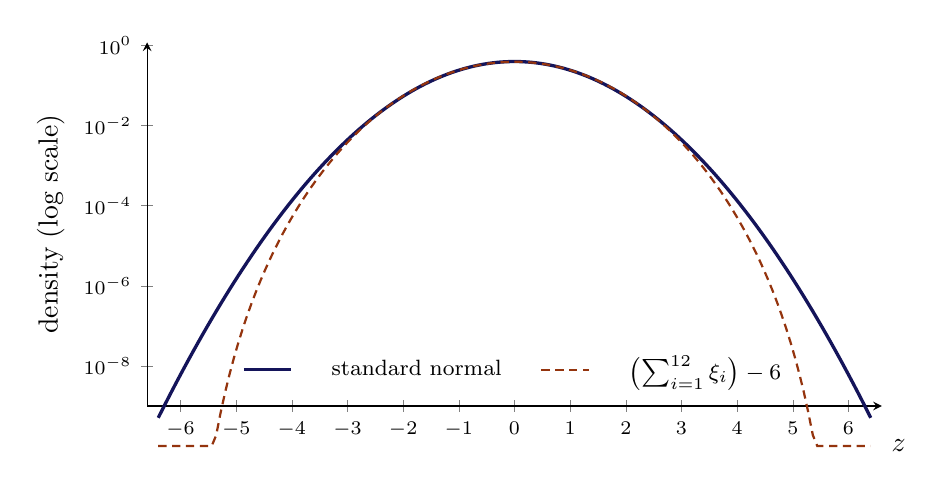
\begin{tikzpicture}
		\begin{axis}[
				width=0.90\textwidth, height=6.2cm,
				ymode=log,
				xmin=-6.6, xmax=6.6, ymin=1e-9, ymax=1.2,
				xtick={-6,-5,-4,-3,-2,-1,0,1,2,3,4,5,6},
				ytick={1e-8,1e-6,1e-4,1e-2,1},
				xlabel={$z$}, ylabel={density (log scale)},
				label style={font=\footnotesize, text=Gray!60!black},
				every axis y label/.style={at={(ticklabel cs:0.5)}, rotate=90,
						anchor=south},
				every axis x label/.style={at={(ticklabel cs:1.0)}, anchor=west},
				axis x line=bottom, axis y line=left,
				axis line style={thin},
				tick label style={font=\scriptsize},
				legend style={font=\footnotesize, at={(0.5,0.03)},
						anchor=south, draw=none, fill=none, legend columns=2,
						column sep=1.2em},
				legend cell align=left,
				clip=false,
			]
			\addplot[MidnightBlue!80!black, very thick] coordinates {
					(-6.40,5.0881e-10) (-6.32,8.4631e-10) (-6.24,1.3987e-09) (-6.16,2.2968e-09) (-6.08,3.7476e-09) (-6.00,6.0759e-09)
					(-5.92,9.7877e-09) (-5.84,1.5667e-08) (-5.76,2.4916e-08) (-5.68,3.9375e-08) (-5.60,6.1826e-08) (-5.52,9.6460e-08)
					(-5.44,1.4953e-07) (-5.36,2.3033e-07) (-5.28,3.5253e-07) (-5.20,5.3610e-07) (-5.12,8.1008e-07) (-5.04,1.2162e-06)
					(-4.96,1.8144e-06) (-4.88,2.6895e-06) (-4.80,3.9613e-06) (-4.72,5.7972e-06) (-4.64,8.4298e-06) (-4.56,1.2180e-05)
					(-4.48,1.7486e-05) (-4.40,2.4942e-05) (-4.32,3.5353e-05) (-4.24,4.9788e-05) (-4.16,6.9670e-05) (-4.08,9.6870e-05)
					(-4.00,1.3383e-04) (-3.92,1.8371e-04) (-3.84,2.5058e-04) (-3.76,3.3960e-04) (-3.68,4.5731e-04) (-3.60,6.1190e-04)
					(-3.52,8.1352e-04) (-3.44,1.0747e-03) (-3.36,1.4106e-03) (-3.28,1.8397e-03) (-3.20,2.3841e-03) (-3.12,3.0698e-03)
					(-3.04,3.9276e-03) (-2.96,4.9929e-03) (-2.88,6.3067e-03) (-2.80,7.9155e-03) (-2.72,9.8712e-03) (-2.64,1.2232e-02)
					(-2.56,1.5060e-02) (-2.48,1.8423e-02) (-2.40,2.2395e-02) (-2.32,2.7048e-02) (-2.24,3.2460e-02) (-2.16,3.8707e-02)
					(-2.08,4.5861e-02) (-2.00,5.3991e-02) (-1.92,6.3157e-02) (-1.84,7.3407e-02) (-1.76,8.4776e-02) (-1.68,9.7282e-02)
					(-1.60,1.1092e-01) (-1.52,1.2566e-01) (-1.44,1.4146e-01) (-1.36,1.5822e-01) (-1.28,1.7585e-01) (-1.20,1.9419e-01)
					(-1.12,2.1307e-01) (-1.04,2.3230e-01) (-0.96,2.5164e-01) (-0.88,2.7086e-01) (-0.80,2.8969e-01) (-0.72,3.0785e-01)
					(-0.64,3.2506e-01) (-0.56,3.4105e-01) (-0.48,3.5553e-01) (-0.40,3.6827e-01) (-0.32,3.7903e-01) (-0.24,3.8762e-01)
					(-0.16,3.9387e-01) (-0.08,3.9767e-01) (0.00,3.9894e-01) (0.08,3.9767e-01) (0.16,3.9387e-01) (0.24,3.8762e-01)
					(0.32,3.7903e-01) (0.40,3.6827e-01) (0.48,3.5553e-01) (0.56,3.4105e-01) (0.64,3.2506e-01) (0.72,3.0785e-01)
					(0.80,2.8969e-01) (0.88,2.7086e-01) (0.96,2.5164e-01) (1.04,2.3230e-01) (1.12,2.1307e-01) (1.20,1.9419e-01)
					(1.28,1.7585e-01) (1.36,1.5822e-01) (1.44,1.4146e-01) (1.52,1.2566e-01) (1.60,1.1092e-01) (1.68,9.7282e-02)
					(1.76,8.4776e-02) (1.84,7.3407e-02) (1.92,6.3157e-02) (2.00,5.3991e-02) (2.08,4.5861e-02) (2.16,3.8707e-02)
					(2.24,3.2460e-02) (2.32,2.7048e-02) (2.40,2.2395e-02) (2.48,1.8423e-02) (2.56,1.5060e-02) (2.64,1.2232e-02)
					(2.72,9.8712e-03) (2.80,7.9155e-03) (2.88,6.3067e-03) (2.96,4.9929e-03) (3.04,3.9276e-03) (3.12,3.0698e-03)
					(3.20,2.3841e-03) (3.28,1.8397e-03) (3.36,1.4106e-03) (3.44,1.0747e-03) (3.52,8.1352e-04) (3.60,6.1190e-04)
					(3.68,4.5731e-04) (3.76,3.3960e-04) (3.84,2.5058e-04) (3.92,1.8371e-04) (4.00,1.3383e-04) (4.08,9.6870e-05)
					(4.16,6.9670e-05) (4.24,4.9788e-05) (4.32,3.5353e-05) (4.40,2.4942e-05) (4.48,1.7486e-05) (4.56,1.2180e-05)
					(4.64,8.4298e-06) (4.72,5.7972e-06) (4.80,3.9613e-06) (4.88,2.6895e-06) (4.96,1.8144e-06) (5.04,1.2162e-06)
					(5.12,8.1008e-07) (5.20,5.3610e-07) (5.28,3.5253e-07) (5.36,2.3033e-07) (5.44,1.4953e-07) (5.52,9.6460e-08)
					(5.60,6.1826e-08) (5.68,3.9375e-08) (5.76,2.4916e-08) (5.84,1.5667e-08) (5.92,9.7877e-09) (6.00,6.0759e-09)
					(6.08,3.7476e-09) (6.16,2.2968e-09) (6.24,1.3987e-09) (6.32,8.4631e-10) (6.40,5.0881e-10)
				};
			\addlegendentry{standard normal}
			\addplot[RawSienna, thick, densely dashed] coordinates {
					(-6.40,1.0000e-10) (-6.32,1.0000e-10) (-6.24,1.0000e-10) (-6.16,1.0000e-10) (-6.08,1.0000e-10) (-6.00,1.0000e-10)
					(-5.92,1.0000e-10) (-5.84,1.0000e-10) (-5.76,1.0000e-10) (-5.68,1.0000e-10) (-5.60,1.0000e-10) (-5.52,1.0000e-10)
					(-5.44,1.0000e-10) (-5.36,1.8485e-10) (-5.28,6.7531e-10) (-5.20,2.1520e-09) (-5.12,6.1398e-09) (-5.04,1.5989e-08)
					(-4.96,3.8567e-08) (-4.88,8.7145e-08) (-4.80,1.8614e-07) (-4.72,3.7858e-07) (-4.64,7.3751e-07) (-4.56,1.3830e-06)
					(-4.48,2.5066e-06) (-4.40,4.4061e-06) (-4.32,7.5335e-06) (-4.24,1.2560e-05) (-4.16,2.0460e-05) (-4.08,3.2626e-05)
					(-4.00,5.1006e-05) (-3.92,7.8283e-05) (-3.84,1.1809e-04) (-3.76,1.7527e-04) (-3.68,2.5618e-04) (-3.60,3.6904e-04)
					(-3.52,5.2435e-04) (-3.44,7.3530e-04) (-3.36,1.0183e-03) (-3.28,1.3933e-03) (-3.20,1.8846e-03) (-3.12,2.5211e-03)
					(-3.04,3.3368e-03) (-2.96,4.3710e-03) (-2.88,5.6690e-03) (-2.80,7.2816e-03) (-2.72,9.2658e-03) (-2.64,1.1684e-02)
					(-2.56,1.4603e-02) (-2.48,1.8094e-02) (-2.40,2.2231e-02) (-2.32,2.7090e-02) (-2.24,3.2747e-02) (-2.16,3.9274e-02)
					(-2.08,4.6739e-02) (-2.00,5.5202e-02) (-1.92,6.4714e-02) (-1.84,7.5312e-02) (-1.76,8.7015e-02) (-1.68,9.9827e-02)
					(-1.60,1.1373e-01) (-1.52,1.2867e-01) (-1.44,1.4459e-01) (-1.36,1.6139e-01) (-1.28,1.7894e-01) (-1.20,1.9710e-01)
					(-1.12,2.1570e-01) (-1.04,2.3453e-01) (-0.96,2.5337e-01) (-0.88,2.7199e-01) (-0.80,2.9014e-01) (-0.72,3.0757e-01)
					(-0.64,3.2402e-01) (-0.56,3.3924e-01) (-0.48,3.5299e-01) (-0.40,3.6504e-01) (-0.32,3.7519e-01) (-0.24,3.8328e-01)
					(-0.16,3.8916e-01) (-0.08,3.9273e-01) (0.00,3.9393e-01) (0.08,3.9273e-01) (0.16,3.8916e-01) (0.24,3.8328e-01)
					(0.32,3.7519e-01) (0.40,3.6504e-01) (0.48,3.5299e-01) (0.56,3.3924e-01) (0.64,3.2402e-01) (0.72,3.0757e-01)
					(0.80,2.9014e-01) (0.88,2.7199e-01) (0.96,2.5337e-01) (1.04,2.3453e-01) (1.12,2.1570e-01) (1.20,1.9710e-01)
					(1.28,1.7894e-01) (1.36,1.6139e-01) (1.44,1.4459e-01) (1.52,1.2867e-01) (1.60,1.1373e-01) (1.68,9.9827e-02)
					(1.76,8.7015e-02) (1.84,7.5312e-02) (1.92,6.4714e-02) (2.00,5.5202e-02) (2.08,4.6739e-02) (2.16,3.9274e-02)
					(2.24,3.2747e-02) (2.32,2.7090e-02) (2.40,2.2231e-02) (2.48,1.8094e-02) (2.56,1.4603e-02) (2.64,1.1684e-02)
					(2.72,9.2658e-03) (2.80,7.2816e-03) (2.88,5.6690e-03) (2.96,4.3710e-03) (3.04,3.3368e-03) (3.12,2.5211e-03)
					(3.20,1.8846e-03) (3.28,1.3933e-03) (3.36,1.0183e-03) (3.44,7.3530e-04) (3.52,5.2435e-04) (3.60,3.6904e-04)
					(3.68,2.5618e-04) (3.76,1.7527e-04) (3.84,1.1809e-04) (3.92,7.8283e-05) (4.00,5.1006e-05) (4.08,3.2626e-05)
					(4.16,2.0460e-05) (4.24,1.2560e-05) (4.32,7.5335e-06) (4.40,4.4061e-06) (4.48,2.5066e-06) (4.56,1.3830e-06)
					(4.64,7.3751e-07) (4.72,3.7858e-07) (4.80,1.8613e-07) (4.88,8.7146e-08) (4.96,3.8568e-08) (5.04,1.5991e-08)
					(5.12,6.1342e-09) (5.20,2.1562e-09) (5.28,6.7169e-10) (5.36,1.8743e-10) (5.44,1.0000e-10) (5.52,1.0000e-10)
					(5.60,1.0000e-10) (5.68,1.0000e-10) (5.76,1.0000e-10) (5.84,1.0000e-10) (5.92,1.0000e-10) (6.00,1.0000e-10)
					(6.08,1.0000e-10) (6.16,1.0000e-10) (6.24,1.0000e-10) (6.32,1.0000e-10) (6.40,1.0000e-10)
				};
			\addlegendentry{$\left(\sum_{i=1}^{12}\xi_{i}\right)-6$}
		\end{axis}
	\end{tikzpicture}
	\caption{Why \eqref{eq:dirty-trick} is only a ballpark approximation. On a
		logarithmic scale the two densities agree to the eye out to about
		$|z|=2$ and then part company: at $z=4$ the trick delivers $38\%$ of the
		correct density, at $z=5$ only $1.7\%$, and beyond $|z|=6$ exactly zero,
		since a sum of twelve uniforms cannot leave $[-6,6]$.}
	\label{fig:dirty-trick}
\end{figure}

\begin{remark}
	這個近似的毛病\emph{正好落在金融最在意的地方}。

	\autoref{fig:dirty-trick} 用對數尺度畫，是因為線性尺度上兩條曲線看起來幾乎重合——中央部分確實吻合得很好。
	問題在尾端：$\sum_{i=1}^{12}\xi_{i}-6$ 的\vocab{支撐集}（support）是 $[-6,6]$，超出範圍的機率\emph{恰好為零}，而真正的常態分佈在那裡仍有 $2\times 10^{-9}$ 的機率。

	回想 \autoref{fig:sp500-density}：真實報酬的尾巴比常態\emph{更厚}。
	若連常態的尾巴都模擬不出來，拿它去算\vocab{風險值}（value at risk, VaR）或\vocab{深度價外}（deep out-of-the-money）選擇權的價格，誤差方向是系統性的——一律低估極端事件。

	所以 J\"ackel 那句「只能用來抓個大概」要認真看待：中央矩（平均、變異數）算得很準，尾端機率則完全不能信。
\end{remark}

%─────§ Bivariate normal────────────────────────────────────────────────────────────────────────────────────────────────────────────────────────────
\section{Generation of Bivariate Normal Distributions}

\source{Slides p.~179}

Pairs of normally distributed variables with correlation $\rho$ can be generated as follows.
Let $X_{1}$ and $X_{2}$ be independent standard normal variables, and set
\begin{equation}
	\begin{aligned}
		U & \;\triangleq\; aX_{1} ,                                   \\
		V & \;\triangleq\; a\rho X_{1} + a\sqrt{1-\rho^{2}}\,X_{2} .
	\end{aligned}\label{eq:bivariate-def}
\end{equation}

\source{Slides p.~180}

\begin{proposition}
	$U$ and $V$ are the desired random variables, with
	\[
		\Var[\,U\,] = \Var[\,V\,] = a^{2} ,
		\qquad
		\Cov[\,U,V\,] = \rho a^{2} .
	\]
\end{proposition}

\begin{proof}
	$\Var[U]=a^{2}\Var[X_{1}]=a^{2}$.
	Since $X_{1}$ and $X_{2}$ are uncorrelated, \eqref{eq:var-sum-uncorr} gives
	\[
		\Var[\,V\,] = a^{2}\rho^{2}\Var[X_{1}] + a^{2}(1-\rho^{2})\Var[X_{2}] = a^{2}\rho^{2}+a^{2}(1-\rho^{2}) = a^{2} .
	\]
	Finally, using $\Cov[X_{1},X_{2}]=0$ and $\Var[X_{1}]=1$,
	\[
		\Cov[\,U,V\,] = a^{2}\rho\,\Var[X_{1}] + a^{2}\sqrt{1-\rho^{2}}\,\Cov[X_{1},X_{2}] = \rho a^{2} . \qedhere
	\]
\end{proof}

Note that the mapping from $(X_{1},X_{2})$ to $(U,V)$ is a one-to-one correspondence for $a\neq 0$.
By \eqref{eq:correlation}, the correlation of $U$ and $V$ is $\rho a^{2}/(a\cdot a)=\rho$, as intended.

\source{Slides p.~181}

The mapping in matrix form is
\begin{equation}
	\begin{bmatrix} U \\ V \end{bmatrix}
	\;=\; a\begin{bmatrix}
		1    & 0                  \\
		\rho & \sqrt{1-\rho^{2}}
	\end{bmatrix}
	\begin{bmatrix} X_{1} \\ X_{2} \end{bmatrix} . \label{eq:bivariate-matrix}
\end{equation}

\begin{figure}[H]
	\centering
	\begin{tikzpicture}
		\begin{groupplot}[
				group style={group size=3 by 1, horizontal sep=1.0cm},
				width=0.345\textwidth, height=3.9cm,
				xmin=-3.4, xmax=3.4, ymin=-3.4, ymax=3.4,
				xtick={-2,0,2}, ytick={-2,0,2},
				axis line style={thin, Gray!70},
				tick label style={font=\scriptsize},
				title style={font=\footnotesize\sffamily, text=MidnightBlue!70!black},
				scatter/use mapped color={draw=MidnightBlue!70, fill=MidnightBlue!30},
			]
			\nextgroupplot[title={$\rho=0$}]
			\addplot[only marks, mark=*, mark size=0.7pt,
				mark options={draw=MidnightBlue!75, fill=MidnightBlue!40}] coordinates {
					(-1.08,-0.98) (2.06,-0.29) (-0.05,0.73) (0.60,0.76) (-0.95,1.78) (0.63,-0.28) (0.44,1.90) (1.49,-1.12)
					(1.59,0.21) (1.82,0.49) (0.07,-0.51) (0.55,-1.95) (-0.05,0.00) (1.39,-0.16) (0.94,1.54) (-0.59,-0.49)
					(0.33,1.07) (0.30,0.94) (0.04,0.87) (-0.17,0.45) (-0.46,0.02) (0.24,-0.06) (-0.18,1.27) (-3.10,1.20)
					(-0.30,-0.75) (-0.15,0.46) (0.86,0.47) (1.33,-1.39) (0.50,0.14) (-0.10,-0.36) (0.43,1.89) (-1.07,-0.67)
					(0.14,-1.20) (-0.31,-0.11) (1.58,-0.58) (-0.93,0.34) (0.30,-1.08) (0.55,-0.11) (0.88,-1.25) (-0.46,1.91)
					(-0.15,0.18) (-0.46,1.22) (0.25,-0.77) (-0.00,0.41) (1.05,-0.08) (-0.49,-2.11) (-1.74,-0.91) (-1.18,-1.40)
					(0.35,0.71) (-0.06,-0.87) (-1.05,-0.24) (1.13,1.41) (-0.44,-1.24) (0.13,1.34) (0.13,-0.35) (0.94,0.45)
					(0.05,0.37) (-0.05,-0.85) (1.01,0.81) (-0.26,-0.67) (1.03,-0.14) (0.52,-0.21) (-0.32,0.40) (-1.05,0.47)
					(0.39,0.46) (0.10,-1.24) (0.45,0.04) (-2.78,-0.72) (-0.69,-1.55) (-0.16,0.72) (-1.67,0.16) (-0.52,-0.38)
					(-0.88,-0.32) (-0.83,-0.13) (1.55,-0.25) (-0.13,-0.31) (1.26,-1.37) (-0.27,-0.96) (-1.09,-0.28) (-0.90,0.25)
					(0.55,-0.41) (1.47,0.70) (0.12,0.25) (0.45,-0.58) (0.62,-0.11) (-0.82,1.51) (0.21,1.20) (-0.05,1.72)
					(-0.99,0.16) (-0.86,-0.59) (-1.02,-0.23) (-0.99,-0.27) (0.07,-1.17) (-1.12,1.48) (0.79,0.53) (0.71,-0.70)
					(1.09,-0.10) (0.76,-0.60) (0.49,-1.47) (0.25,0.62) (1.05,1.09) (1.47,-1.18) (-1.63,-0.62) (1.29,-1.30)
					(-0.20,-0.08) (0.57,0.94) (0.34,0.21) (0.34,-0.52) (0.52,-0.88) (-0.56,-0.16) (0.74,-0.39) (0.75,-0.75)
					(-0.56,-0.75) (-0.52,0.47) (-1.82,-0.25) (-1.14,0.20) (1.19,0.26) (0.05,1.61) (0.06,-1.06) (0.90,-0.94)
					(-0.07,0.24) (-0.55,-0.31) (0.46,0.24) (-1.94,-1.09) (-0.87,0.05) (1.07,-0.88) (0.05,-0.44) (-1.46,-1.55)
					(0.00,0.62) (0.52,0.41) (-0.18,-0.96) (-0.32,1.10) (1.19,-0.09) (0.32,0.45) (0.17,-0.07) (0.89,0.63)
					(-0.68,-0.28) (-1.15,-0.98) (-0.40,-0.42) (-1.07,-0.92) (0.12,-0.63) (-0.84,-0.53) (0.79,1.64) (-0.91,1.06)
					(-2.57,0.09) (-0.22,-0.39) (-0.38,0.09) (-0.60,-0.65) (-0.22,-0.54) (-0.26,-0.86)
				};
			\nextgroupplot[title={$\rho=0.6$}]
			\addplot[only marks, mark=*, mark size=0.7pt,
				mark options={draw=MidnightBlue!75, fill=MidnightBlue!40}] coordinates {
					(-1.08,-1.43) (2.06,1.00) (-0.05,0.56) (0.60,0.97) (-0.95,0.85) (0.63,0.16) (0.44,1.78) (1.49,-0.00)
					(1.59,1.12) (1.82,1.48) (0.07,-0.36) (0.55,-1.23) (-0.05,-0.03) (1.39,0.70) (0.94,1.79) (-0.59,-0.75)
					(0.33,1.06) (0.30,0.93) (0.04,0.72) (-0.17,0.26) (-0.46,-0.26) (0.24,0.09) (-0.18,0.91) (-3.10,-0.90)
					(-0.30,-0.78) (-0.15,0.27) (0.86,0.89) (1.33,-0.31) (0.50,0.41) (-0.10,-0.35) (0.43,1.77) (-1.07,-1.18)
					(0.14,-0.88) (-0.31,-0.27) (1.58,0.49) (-0.93,-0.28) (0.30,-0.69) (0.55,0.24) (0.88,-0.47) (-0.46,1.25)
					(-0.15,0.05) (-0.46,0.70) (0.25,-0.46) (-0.00,0.33) (1.05,0.56) (-0.49,-1.98) (-1.74,-1.77) (-1.18,-1.83)
					(0.35,0.77) (-0.06,-0.73) (-1.05,-0.82) (1.13,1.81) (-0.44,-1.26) (0.13,1.15) (0.13,-0.20) (0.94,0.92)
					(0.05,0.33) (-0.05,-0.72) (1.01,1.25) (-0.26,-0.69) (1.03,0.50) (0.52,0.14) (-0.32,0.12) (-1.05,-0.25)
					(0.39,0.60) (0.10,-0.93) (0.45,0.30) (-2.78,-2.24) (-0.69,-1.66) (-0.16,0.48) (-1.67,-0.88) (-0.52,-0.62)
					(-0.88,-0.78) (-0.83,-0.60) (1.55,0.73) (-0.13,-0.33) (1.26,-0.33) (-0.27,-0.93) (-1.09,-0.88) (-0.90,-0.34)
					(0.55,0.00) (1.47,1.44) (0.12,0.27) (0.45,-0.19) (0.62,0.28) (-0.82,0.72) (0.21,1.08) (-0.05,1.35)
					(-0.99,-0.46) (-0.86,-0.99) (-1.02,-0.79) (-0.99,-0.81) (0.07,-0.90) (-1.12,0.51) (0.79,0.90) (0.71,-0.13)
					(1.09,0.57) (0.76,-0.02) (0.49,-0.88) (0.25,0.65) (1.05,1.50) (1.47,-0.06) (-1.63,-1.47) (1.29,-0.27)
					(-0.20,-0.18) (0.57,1.09) (0.34,0.37) (0.34,-0.21) (0.52,-0.39) (-0.56,-0.46) (0.74,0.13) (0.75,-0.15)
					(-0.56,-0.94) (-0.52,0.07) (-1.82,-1.29) (-1.14,-0.52) (1.19,0.93) (0.05,1.32) (0.06,-0.81) (0.90,-0.21)
					(-0.07,0.15) (-0.55,-0.58) (0.46,0.47) (-1.94,-2.04) (-0.87,-0.48) (1.07,-0.06) (0.05,-0.32) (-1.46,-2.12)
					(0.00,0.50) (0.52,0.64) (-0.18,-0.87) (-0.32,0.68) (1.19,0.64) (0.32,0.56) (0.17,0.05) (0.89,1.04)
					(-0.68,-0.63) (-1.15,-1.48) (-0.40,-0.58) (-1.07,-1.38) (0.12,-0.43) (-0.84,-0.93) (0.79,1.78) (-0.91,0.30)
					(-2.57,-1.47) (-0.22,-0.44) (-0.38,-0.16) (-0.60,-0.88) (-0.22,-0.56) (-0.26,-0.84)
				};
			\nextgroupplot[title={$\rho=0.95$}]
			\addplot[only marks, mark=*, mark size=0.7pt,
				mark options={draw=MidnightBlue!75, fill=MidnightBlue!40}] coordinates {
					(-1.08,-1.33) (2.06,1.87) (-0.05,0.18) (0.60,0.81) (-0.95,-0.35) (0.63,0.51) (0.44,1.01) (1.49,1.07)
					(1.59,1.58) (1.82,1.88) (0.07,-0.09) (0.55,-0.09) (-0.05,-0.05) (1.39,1.27) (0.94,1.37) (-0.59,-0.71)
					(0.33,0.65) (0.30,0.58) (0.04,0.31) (-0.17,-0.02) (-0.46,-0.43) (0.24,0.21) (-0.18,0.23) (-3.10,-2.57)
					(-0.30,-0.52) (-0.15,-0.00) (0.86,0.96) (1.33,0.83) (0.50,0.52) (-0.10,-0.21) (0.43,1.00) (-1.07,-1.23)
					(0.14,-0.24) (-0.31,-0.33) (1.58,1.32) (-0.93,-0.78) (0.30,-0.06) (0.55,0.49) (0.88,0.44) (-0.46,0.16)
					(-0.15,-0.09) (-0.46,-0.06) (0.25,0.00) (-0.00,0.13) (1.05,0.97) (-0.49,-1.12) (-1.74,-1.93) (-1.18,-1.56)
					(0.35,0.55) (-0.06,-0.33) (-1.05,-1.07) (1.13,1.52) (-0.44,-0.81) (0.13,0.54) (0.13,0.01) (0.94,1.03)
					(0.05,0.17) (-0.05,-0.32) (1.01,1.21) (-0.26,-0.46) (1.03,0.93) (0.52,0.43) (-0.32,-0.18) (-1.05,-0.85)
					(0.39,0.51) (0.10,-0.29) (0.45,0.44) (-2.78,-2.87) (-0.69,-1.14) (-0.16,0.07) (-1.67,-1.54) (-0.52,-0.61)
					(-0.88,-0.93) (-0.83,-0.83) (1.55,1.39) (-0.13,-0.22) (1.26,0.77) (-0.27,-0.56) (-1.09,-1.13) (-0.90,-0.77)
					(0.55,0.39) (1.47,1.61) (0.12,0.19) (0.45,0.24) (0.62,0.55) (-0.82,-0.30) (0.21,0.57) (-0.05,0.49)
					(-0.99,-0.89) (-0.86,-1.00) (-1.02,-1.04) (-0.99,-1.03) (0.07,-0.30) (-1.12,-0.60) (0.79,0.92) (0.71,0.45)
					(1.09,1.00) (0.76,0.53) (0.49,0.01) (0.25,0.43) (1.05,1.34) (1.47,1.03) (-1.63,-1.74) (1.29,0.82)
					(-0.20,-0.22) (0.57,0.83) (0.34,0.39) (0.34,0.16) (0.52,0.22) (-0.56,-0.58) (0.74,0.58) (0.75,0.48)
					(-0.56,-0.76) (-0.52,-0.34) (-1.82,-1.80) (-1.14,-1.02) (1.19,1.22) (0.05,0.55) (0.06,-0.27) (0.90,0.56)
					(-0.07,0.01) (-0.55,-0.62) (0.46,0.52) (-1.94,-2.18) (-0.87,-0.81) (1.07,0.74) (0.05,-0.09) (-1.46,-1.87)
					(0.00,0.20) (0.52,0.62) (-0.18,-0.47) (-0.32,0.04) (1.19,1.10) (0.32,0.45) (0.17,0.14) (0.89,1.04)
					(-0.68,-0.73) (-1.15,-1.40) (-0.40,-0.51) (-1.07,-1.31) (0.12,-0.08) (-0.84,-0.96) (0.79,1.26) (-0.91,-0.53)
					(-2.57,-2.41) (-0.22,-0.33) (-0.38,-0.33) (-0.60,-0.77) (-0.22,-0.37) (-0.26,-0.52)
				};
		\end{groupplot}
	\end{tikzpicture}
	\caption{Bivariate normal samples generated by
		\eqref{eq:bivariate-matrix} with $a=1$, from the same underlying
		$(X_{1},X_{2})$ draws. Raising $\rho$ shears the cloud towards the diagonal
		without changing either marginal.}
	\label{fig:bivariate}
\end{figure}

\begin{remark}
	\eqref{eq:bivariate-matrix} 不是特例，而是一般作法的二維版本。

	那個下三角矩陣正是相關係數矩陣
	$\begin{bmatrix}1 & \rho\\ \rho & 1\end{bmatrix}$
	的 \vocab{Cholesky 分解}（Cholesky decomposition）$LL^{\mathsf{T}}$：
	\[
		L = \begin{bmatrix} 1 & 0 \\ \rho & \sqrt{1-\rho^{2}} \end{bmatrix},
		\qquad
		LL^{\mathsf{T}} = \begin{bmatrix} 1 & \rho \\ \rho & 1 \end{bmatrix} .
	\]
	一般地，要產生共變異數矩陣為 $C$ 的 $n$ 維常態向量，就把 $C$ 做 Cholesky 分解 $C=LL^{\mathsf{T}}$，取獨立標準常態向量 $\bm{X}$，令 $\bm{U}=L\bm{X}$；則
	$\Cov[\bm{U}]=L\,\Cov[\bm{X}]\,L^{\mathsf{T}}=LL^{\mathsf{T}}=C$。

	這也解釋了 \eqref{eq:mvn-pdf} 為什麼要求 $C$ \vocab{正定}（positive definite）——正定才有 Cholesky 分解，才產得出來。
	實務上由市場資料估出的相關係數矩陣常因雜訊而不正定，必須先做修正，否則模擬根本無法開始。
\end{remark}

%─────§ Lognormal──────────────────────────────────────────────────────────────────────────────────────────────────────────────────────────────────
\section{The Lognormal Distribution}
\label{sec:lognormal}

\source{Slides p.~182}

\begin{definition}
	A random variable $Y$ is said to have a \vocab{lognormal distribution} if $\ln Y$ has a normal distribution.
\end{definition}

Let $X\sim N(\mu,\sigma^{2})$ and $Y\triangleq e^{X}$.
The mean and variance of $Y$ are
\begin{equation}
	\begin{aligned}
		\mu_{Y}      & \;=\; e^{\mu+\sigma^{2}/2} ,                          \\
		\sigma_{Y}^{2} & \;=\; e^{2\mu+\sigma^{2}}\bigl(e^{\sigma^{2}}-1\bigr) ,
	\end{aligned}\label{eq:lognormal-moments}
\end{equation}
respectively.
They follow from $E[\,Y^{n}\,]=e^{n\mu+n^{2}\sigma^{2}/2}$ --- which is just \eqref{eq:normal-mgf} evaluated at $t=n$.

\begin{figure}[H]
	\centering
	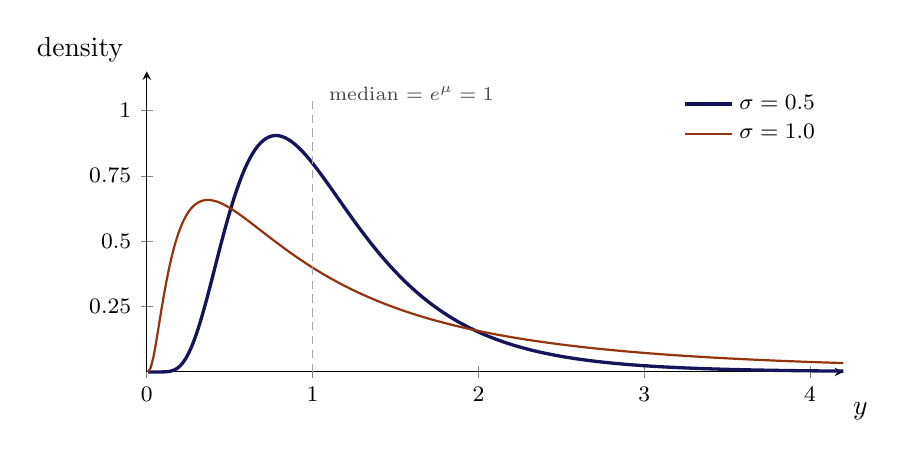
\begin{tikzpicture}
		\begin{axis}[
				width=0.86\textwidth, height=5.4cm,
				xmin=0, xmax=4.2, ymin=0, ymax=1.15,
				xtick={0,1,2,3,4}, ytick={0.25,0.5,0.75,1.0},
				yticklabel style={/pgf/number format/fixed,
						/pgf/number format/precision=2},
				xlabel={$y$}, ylabel={density},
				label style={font=\footnotesize, text=Gray!60!black},
				every axis y label/.style={at={(ticklabel cs:1.0)}, rotate=0, anchor=south},
				every axis x label/.style={at={(ticklabel cs:1.0)}, anchor=west},
				axis x line=bottom, axis y line=left,
				axis line style={thin},
				tick label style={font=\footnotesize},
				legend style={font=\footnotesize, at={(0.98,0.96)},
						anchor=north east, draw=none, fill=none},
				legend cell align=left,
				clip=false,
			]
			\addplot[MidnightBlue!80!black, very thick, domain=0.008:4.2, samples=260]
			{exp(-(ln(x))^2/(2*0.25))/(x*0.5*sqrt(2*pi))};
			\addlegendentry{$\sigma=0.5$}
			\addplot[RawSienna, thick, domain=0.008:4.2, samples=260]
			{exp(-(ln(x))^2/(2*1.0))/(x*1.0*sqrt(2*pi))};
			\addlegendentry{$\sigma=1.0$}
			\addplot[Gray!70, densely dashed, domain=0.008:4.2, samples=2]
			coordinates {(1,0) (1,1.05)};
			\node[font=\scriptsize, text=Gray!55!black, anchor=south west]
			at (axis cs:1.04,1.0) {median $=e^{\mu}=1$};
		\end{axis}
	\end{tikzpicture}
	\caption{Lognormal densities with $\mu=0$. The support is $(0,\infty)$, the
		shape is right-skewed, and the right tail thickens rapidly with $\sigma$.
		The median sits at $e^{\mu}$ regardless of $\sigma$, while the mean
		$e^{\mu+\sigma^{2}/2}$ drifts to the right of it.}
	\label{fig:lognormal}
\end{figure}

\begin{remark}
	為什麼金融上用\vocab{對數常態分佈}（lognormal distribution）描述\emph{價格}，用常態描述\emph{對數報酬}？三個理由，都看得見。

	\textbf{（一）價格不能為負。}
	常態分佈的支撐集是整條實線，但股價不會是負的。
	$Y=e^{X}$ 自動把值域限制在 $(0,\infty)$。

	\textbf{（二）報酬可加，價格可乘。}
	回顧 \autoref{sec:log-returns} 的對數報酬 $r_{t}=\ln(S_{t}/S_{t-1})$：跨期報酬是逐期報酬之\emph{和}。
	若每期 $r_{t}$ 為獨立常態，其和仍為常態，於是 $S_{T}=S_{0}\exp(\sum r_{t})$ 必然是對數常態。
	這個封閉性正是整個模型的骨架。

	\textbf{（三）平均數與中位數不同。}
	\eqref{eq:lognormal-moments} 裡的 $\mu_{Y}=e^{\mu+\sigma^{2}/2}$ 嚴格大於\vocab{中位數}（median）$e^{\mu}$，差額 $\sigma^{2}/2$ 純粹來自\emph{波動本身}。
	這就是日後反覆出現的「$-\sigma^{2}/2$ 修正項」的來源：想讓價格的\emph{期望}成長率等於 $r$，指數裡就得寫 $r-\sigma^{2}/2$。
	這又是 Jensen 不等式（見 \autoref{sec:ts-theories} 的「壞」預期理論）的另一個面貌。
\end{remark}

\source{Slides p.~183}

Conversely, suppose $Y$ is lognormally distributed with mean $\mu$ and variance $\sigma^{2}$.
Then $\ln Y$ has a normal distribution with
\begin{equation}
	\begin{aligned}
		E[\,\ln Y\,]    & \;=\; \ln\left[\,\mu\big/\sqrt{1+(\sigma/\mu)^{2}}\,\right] , \\
		\Var[\,\ln Y\,] & \;=\; \ln\bigl[\,1+(\sigma/\mu)^{2}\,\bigr] .
	\end{aligned}\label{eq:lognormal-inverse}
\end{equation}

If $X$ and $Y$ are joint-lognormally distributed, then
\begin{equation}
	\begin{aligned}
		E[\,XY\,]      & \;=\; E[\,X\,]E[\,Y\,]\,e^{\Cov[\,\ln X,\ln Y\,]} ,                     \\
		\Cov[\,X,Y\,]  & \;=\; E[\,X\,]E[\,Y\,]\left(e^{\Cov[\,\ln X,\ln Y\,]}-1\right) .
	\end{aligned}\label{eq:joint-lognormal}
\end{equation}

\begin{note}
	Beware the notation on this page: $\mu$ and $\sigma^{2}$ now denote the mean and variance of $Y$ \emph{itself}, not of $\ln Y$ as on the previous page.
	\eqref{eq:lognormal-inverse} is the inverse of \eqref{eq:lognormal-moments}, and the two must not be mixed.
	A quick check: substituting $\mu=e^{m+s^{2}/2}$ and $\sigma^{2}=e^{2m+s^{2}}(e^{s^{2}}-1)$ into \eqref{eq:lognormal-inverse} returns $E[\ln Y]=m$ and $\Var[\ln Y]=s^{2}$, as it should.
\end{note}

\source{Slides p.~184}

\begin{theorem}
	Let $Y$ be lognormally distributed such that $\ln Y\sim N(\mu,\sigma^{2})$, with density $f$. Then
	\begin{equation}
		\int_{a}^{\infty} y\,f(y)\,dy
		\;=\; e^{\mu+\sigma^{2}/2}\,N\!\left(\frac{\mu-\ln a}{\sigma}+\sigma\right) . \label{eq:lognormal-partial}
	\end{equation}
\end{theorem}

\begin{proof}
	Substitute $y=e^{x}$, so that $\ln Y = X\sim N(\mu,\sigma^{2})$ and the integral becomes
	\[
		\int_{\ln a}^{\infty} e^{x}\,\frac{1}{\sigma\sqrt{2\pi}}\,e^{-(x-\mu)^{2}/(2\sigma^{2})}\,dx .
	\]
	Completing the square in the exponent,
	\[
		x - \frac{(x-\mu)^{2}}{2\sigma^{2}}
		= \mu + \frac{\sigma^{2}}{2} - \frac{\bigl(x-\mu-\sigma^{2}\bigr)^{2}}{2\sigma^{2}} ,
	\]
	so the integral equals
	\[
		e^{\mu+\sigma^{2}/2}\int_{\ln a}^{\infty}\frac{1}{\sigma\sqrt{2\pi}}\,
		e^{-(x-\mu-\sigma^{2})^{2}/(2\sigma^{2})}\,dx
		= e^{\mu+\sigma^{2}/2}\;\mathrm{Prob}\bigl[\,Z > \tfrac{\ln a-\mu-\sigma^{2}}{\sigma}\,\bigr] ,
	\]
	with $Z$ standard normal.
	By the symmetry $1-N(z)=N(-z)$ this is $e^{\mu+\sigma^{2}/2}N\bigl((\mu+\sigma^{2}-\ln a)/\sigma\bigr)$, which is \eqref{eq:lognormal-partial}.
\end{proof}

\begin{moral}
	\eqref{eq:lognormal-partial} is the \vocab{partial expectation} of a lognormal variable --- the expected value of $Y$ restricted to the event $Y>a$.

	It is not a technical curiosity: it is the entire content of the first term of the Black--Scholes formula.
	A call option pays $Y-a$ exactly when $Y>a$, so its expected payoff splits into
	$\int_{a}^{\infty}y\,f(y)\,dy - a\,\mathrm{Prob}[\,Y>a\,]$ ---
	the first piece supplying $S_{0}N(d_{1})$ and the second $a\,N(d_{2})$.
	Every remaining chapter of this course is, in one way or another, an elaboration of that split.

	\eqref{eq:lognormal-partial} 就是 Black--Scholes 公式第一項的全部內容；買權在 $Y>a$ 時付 $Y-a$，期望報酬拆成這兩塊，前者給出 $S_{0}N(d_{1})$，後者給出 $a\,N(d_{2})$。
\end{moral}
